\chapter{Combined \vhbc\ Analysis Appendix}
\ChapFrame

\textit{This Appendix lists some additional results in support of Chapter \ref{chap-VH}.}

% Trigger to technical
%\section{Triggers}\label{appsec-trigger}
%This section gives further details on the triggers used in the combined analysis presented in Chapter \ref{chap-VH}.
%\begin{table}[!htpb]
    \begin{center}
      \scriptsize
      \resizebox{\textwidth}{!}{
        \begin{tabular}{c|c|c|c|p{7.2cm}} \hline \hline
           \textbf{ Type } & \textbf{ Trigger Name }        &     \textbf{Period}     &  \textbf{Threshold}     &     \textbf{Description}               
          \\ \hline \hline
          \multirow{5}{*}{$\etm$}  
          & HLT\_xe70\_L1XE50         &      2015               &      70 GeV                    &    
          \multirow{5}{*}{\parbox{6.6cm}{Seeded using the level L1\_XE50 (L1\_XE55) LAr and Tile calorimeter triggers, 
                          calibrated at the EM scale, with a threshold of 50(55) GeV.}} \\
          & HLT\_xe90\_mht\_L1XE50         &      2016 (A-D3)               &      90 GeV                    &     \\
          & HLT\_xe110\_mht\_L1XE50        &      2016 ($\geq$ D4)              &      110 GeV                   &     \\
          & HLT\_xe110\_pufit\_L1XE55        &      2017               &      110 GeV                   &    \\
          & HLT\_xe110\_pufit\_xe70\_L1XE50        &      2018               &      110 GeV                   &    \\
          \hline \hline
          \multirow{7}{*}{Electron}  
          & HLT\_e24\_lhmedium\_L1EM20VH  &  2015  &   24 GeV    &    Seeded using L1 EM20VH level 1 trigger calibrated at the EM scale with a threshold of 20 GeV, require likelihood medium ID.\\
          & HLT\_e60\_lhmedium            &  2015  &   60 GeV    &    Require likelihood medium ID.\\
          & HLT\_e120\_lhloose            &  2015  &  120 GeV    &    Require likelihood loose ID.\\
          & HLT\_e26\_lhtight\_nod0\_ivarloose  &      2016 -- 2018         &         26 GeV     &    Tight likelihood ID required, alignment-robust likelihood tune with no d0 information used, and variable loose isolation required\\
          & HLT\_e60\_lhmedium(\_nod0)           &      2016 -- 2018        &         60 GeV     &    Medium ID likelihood required\\
          & HLT\_e140\_lhloose(\_nod0)           &      2016 -- 2018        &         140 GeV    &    Loose ID likelihood required\\
          & HLT\_e300\_etcut                     &      2018                &         300 GeV    &    No ID requirements. \\
          \hline \hline
          \multirow{3}{*}{Muon}  
          & HLT\_mu20\_iloose\_L1MU15      &      2015           &  20 GeV &   Seeded using L1MU15 level 1 trigger with a threshold of 15 GeV, and requiring loose isolation requirements.\\
          & HLT\_mu50\                     &      2015 -- 2018   &  50 GeV &   No isolation requirements. \\
          & HLT\_mu26\_ivarmedium          &      2016 -- 2018   &  26 GeV &   Variable cone medium isolation requirements \\
          \hline \hline
        \end{tabular}
      }
      \caption{Triggers used during the 2015-2018 data collection period, from the internal documentation.
               For the HLT that L1 trigger is not mentioned, the default L1 trigger is used. 
               The default L1 trigger is EM22VHI or EM24VHI for single electron, 
               MU20 or MU21 for single muon, depends on the data taken period
               \cite{TwikiTriggerNamingRun2}. }
      \label{tab:trigs2015_to_2018}
    \end{center}
  \end{table}

\section{Flavour Tagging Calibrations}\label{appsec-vh-ftagcal}
This section presents some results on the calibration of the flavour tagger used in the combined \vhbc\ analysis. Figure \ref{appfig:FTAG_calibration_resolved} shows some efficiency scale factors in the resolved regime for the different main flavours, while Figure \ref{appfig:FTAG_calibration_boosted} displays the same information for the boosted tagger.

\begin{figure}
    \centering
    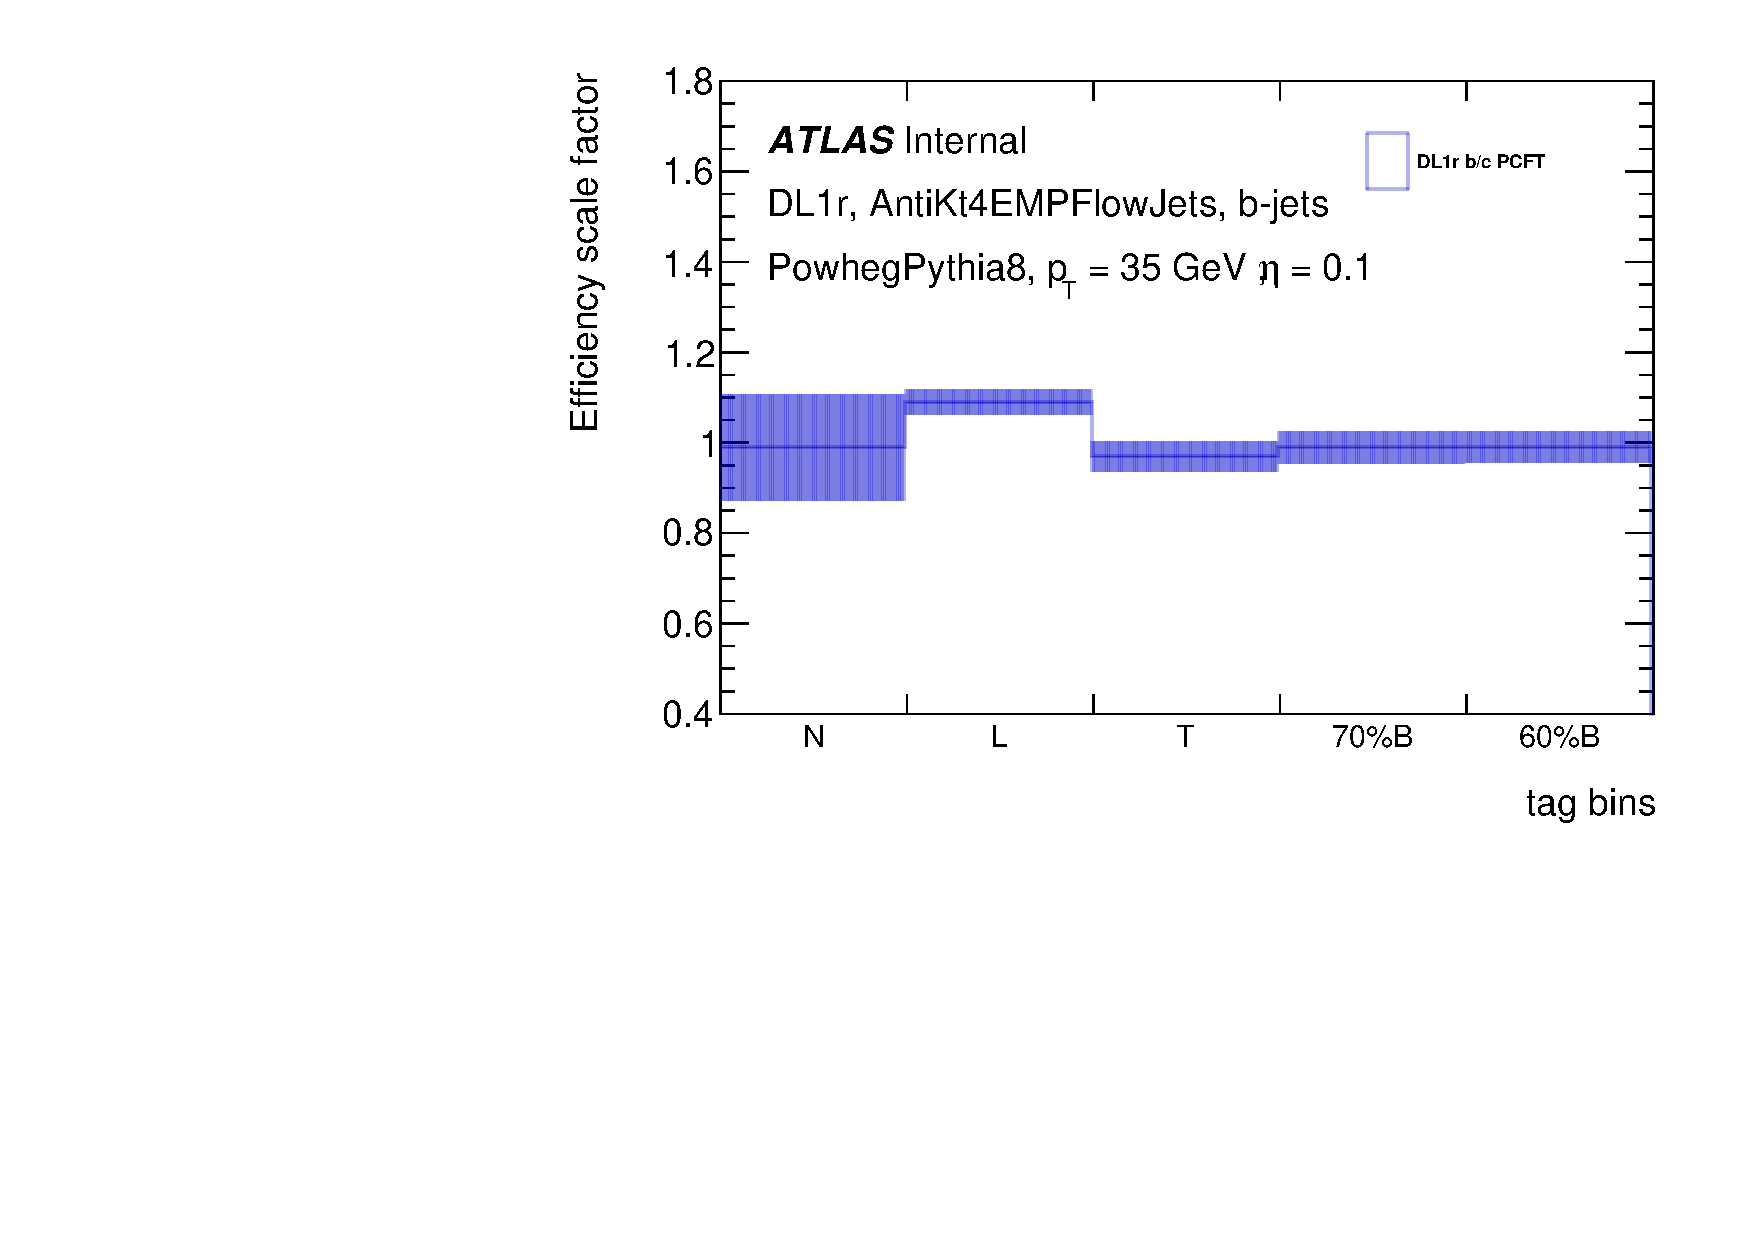
\includegraphics[width=0.48\textwidth]{Images/VH/Obj/FTAGCalib/ftagres/DL1r_AntiKt4EMPFlowJets_BTagging201903_Continuous2D_B_410470_30_eta01.pdf}
    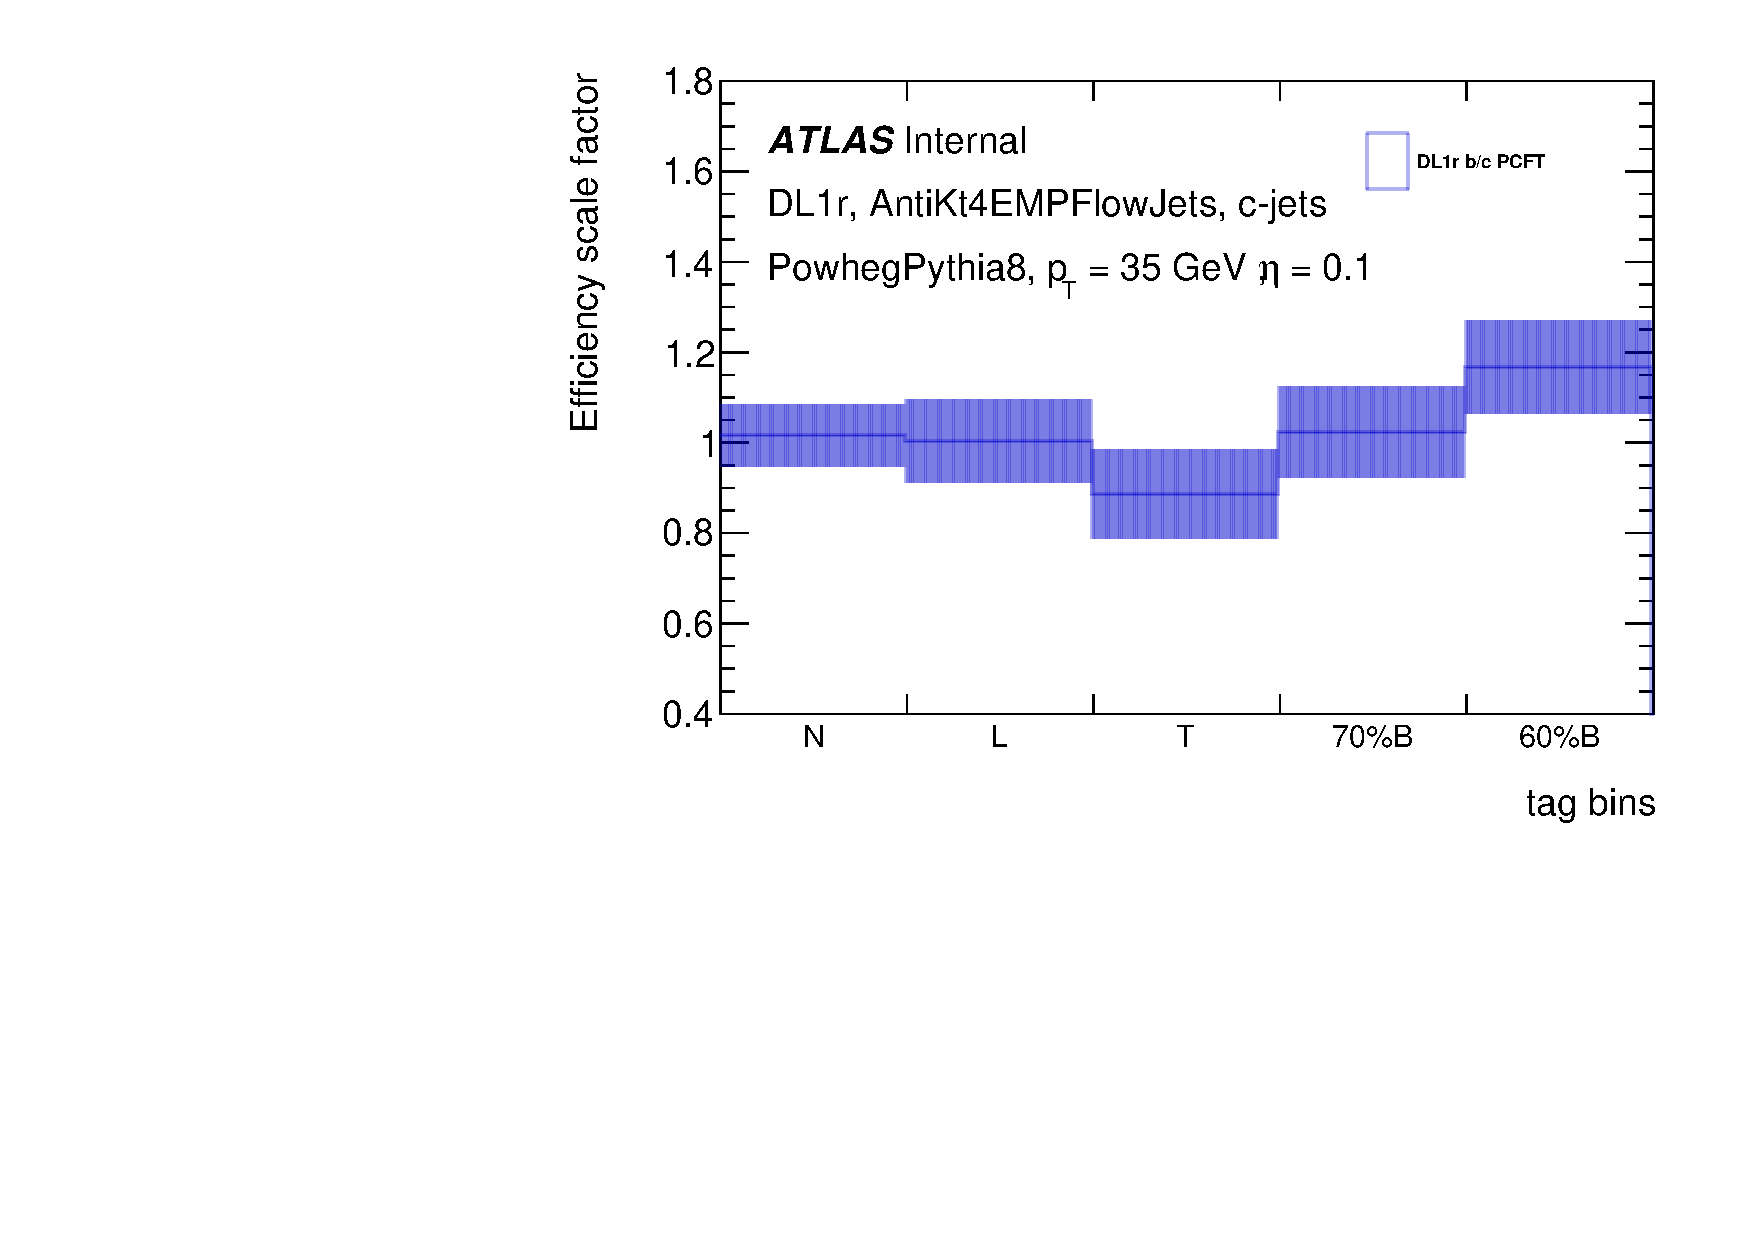
\includegraphics[width=0.48\textwidth]{Images/VH/Obj/FTAGCalib/ftagres/DL1r_AntiKt4EMPFlowJets_BTagging201903_Continuous2D_C_410470_30_eta01.pdf}\\
    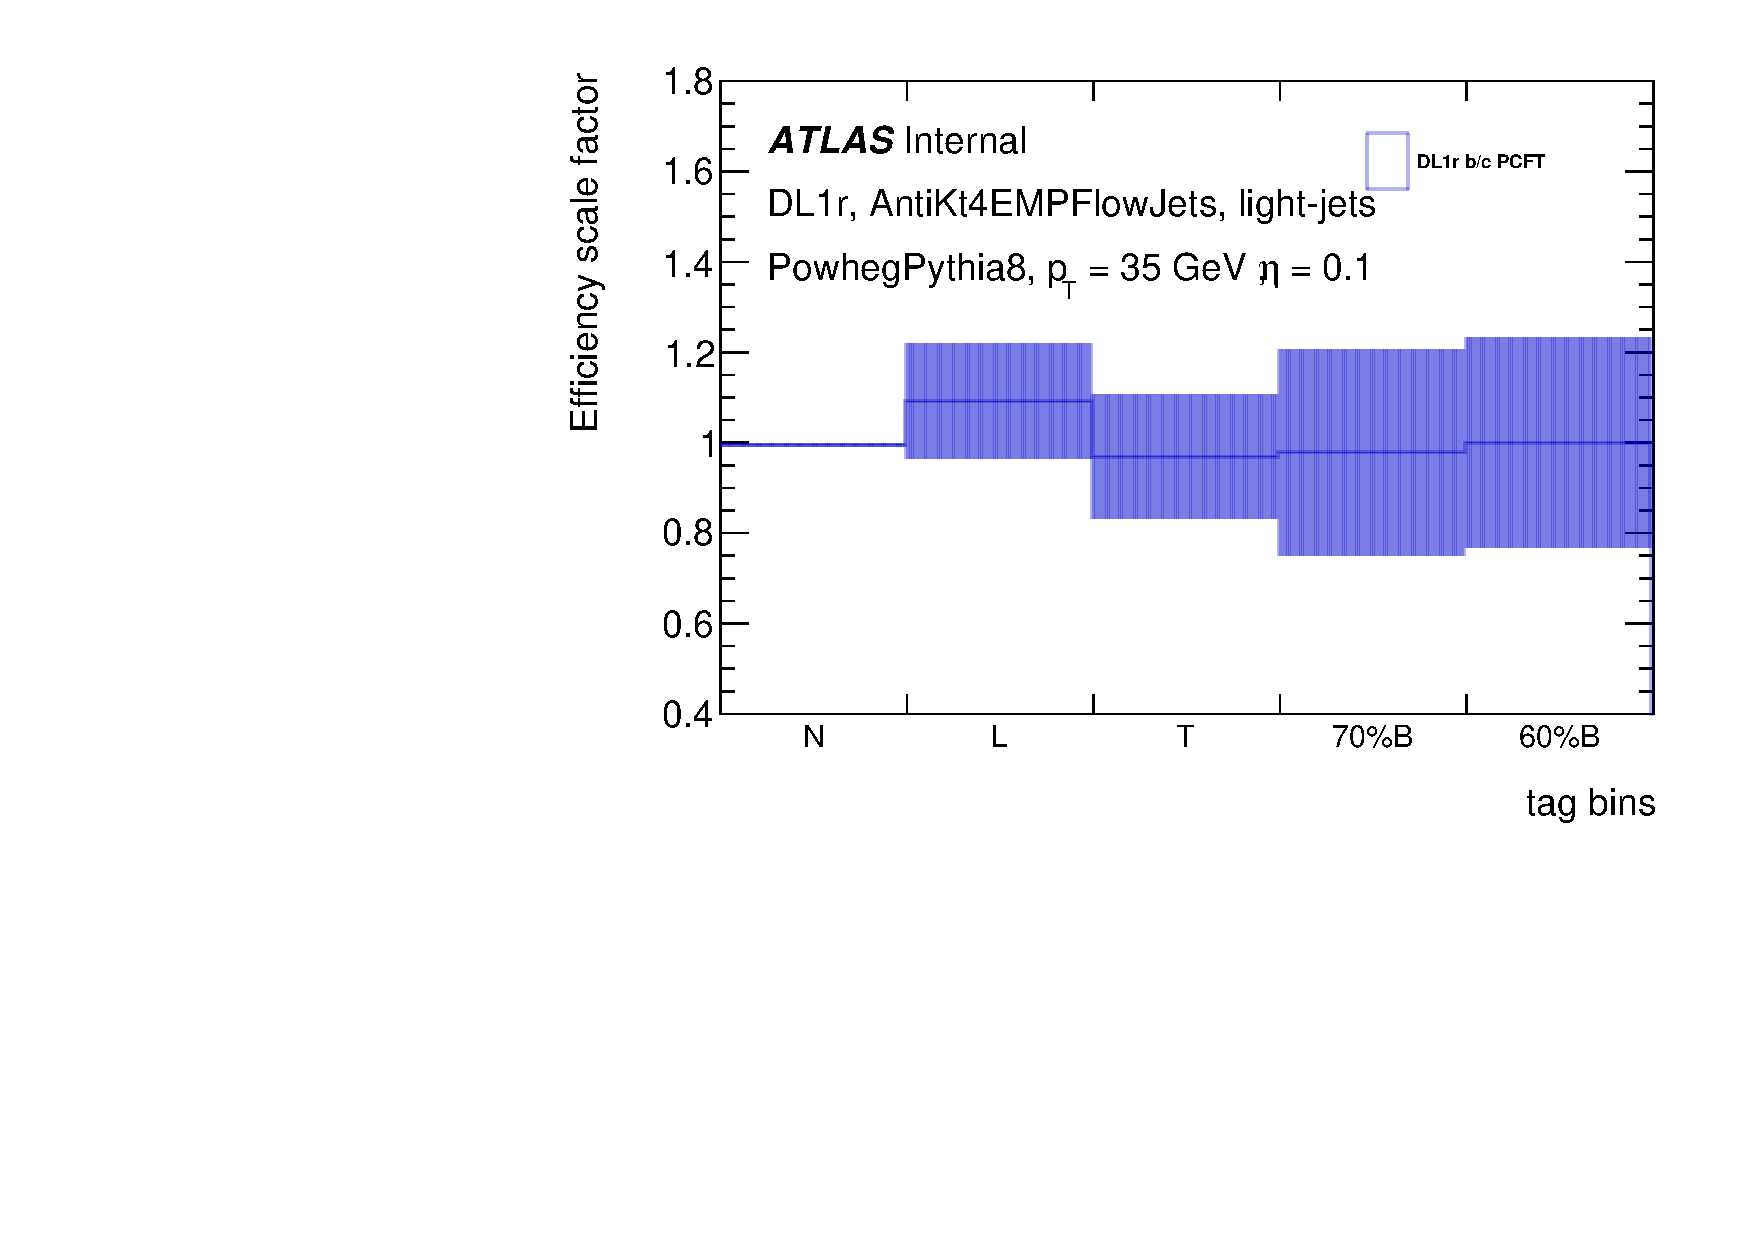
\includegraphics[width=0.48\textwidth]{Images/VH/Obj/FTAGCalib/ftagres/DL1r_AntiKt4EMPFlowJets_BTagging201903_Continuous2D_Light_410470_30_eta01.pdf}
    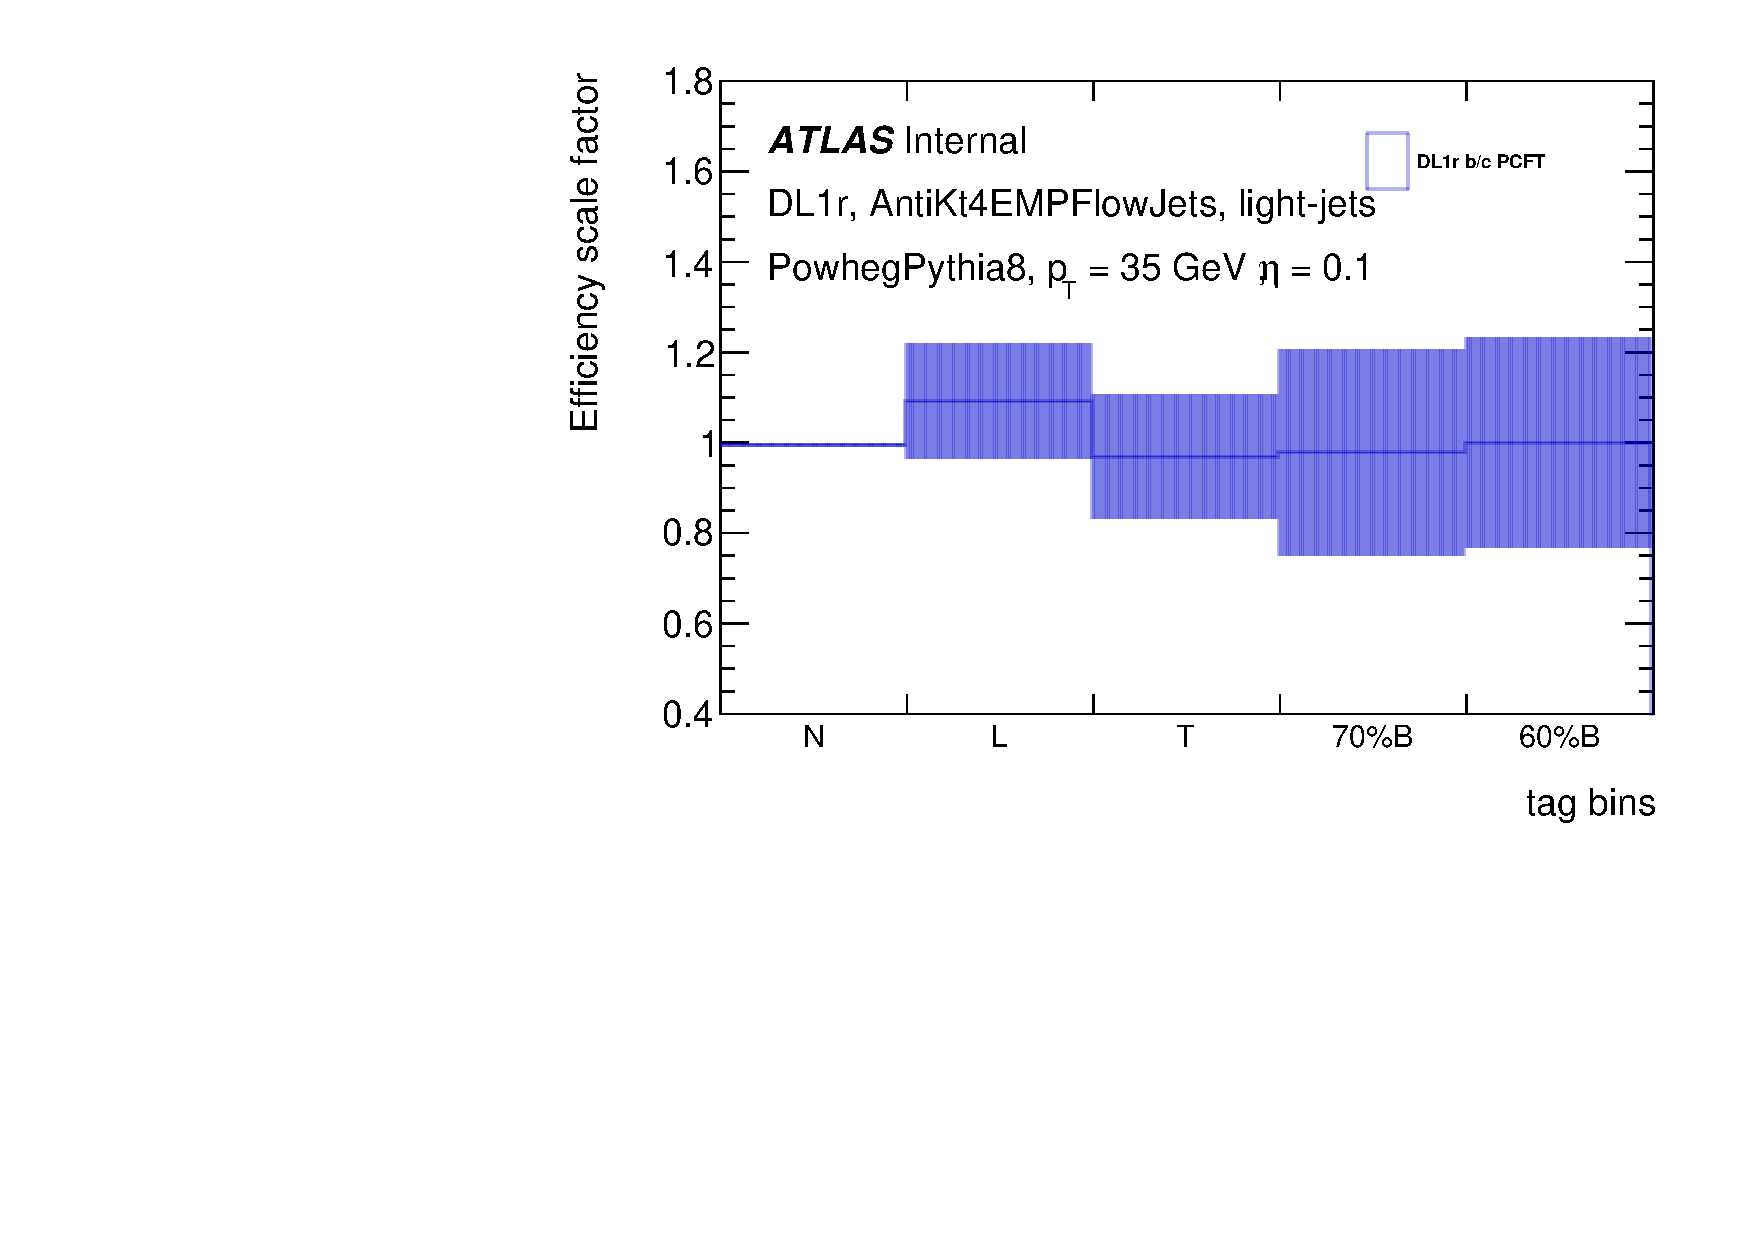
\includegraphics[width=0.48\textwidth]{Images/VH/Obj/FTAGCalib/ftagres/DL1r_AntiKt4EMPFlowJets_BTagging201903_Continuous2D_Light_410470_30_eta01.pdf}
    \caption{Efficiency scale factors calibration results of the DL1r \gls{pcft} tagger on PowhegPythia8 \ttb\ samples for the resolved regime of the \vhbc. The scale factors of $\tau$-jets are from $c$-jet calibration. From the internal documentation.
    }
    \label{appfig:FTAG_calibration_resolved}
\end{figure}
   
\begin{figure}
    \centering
    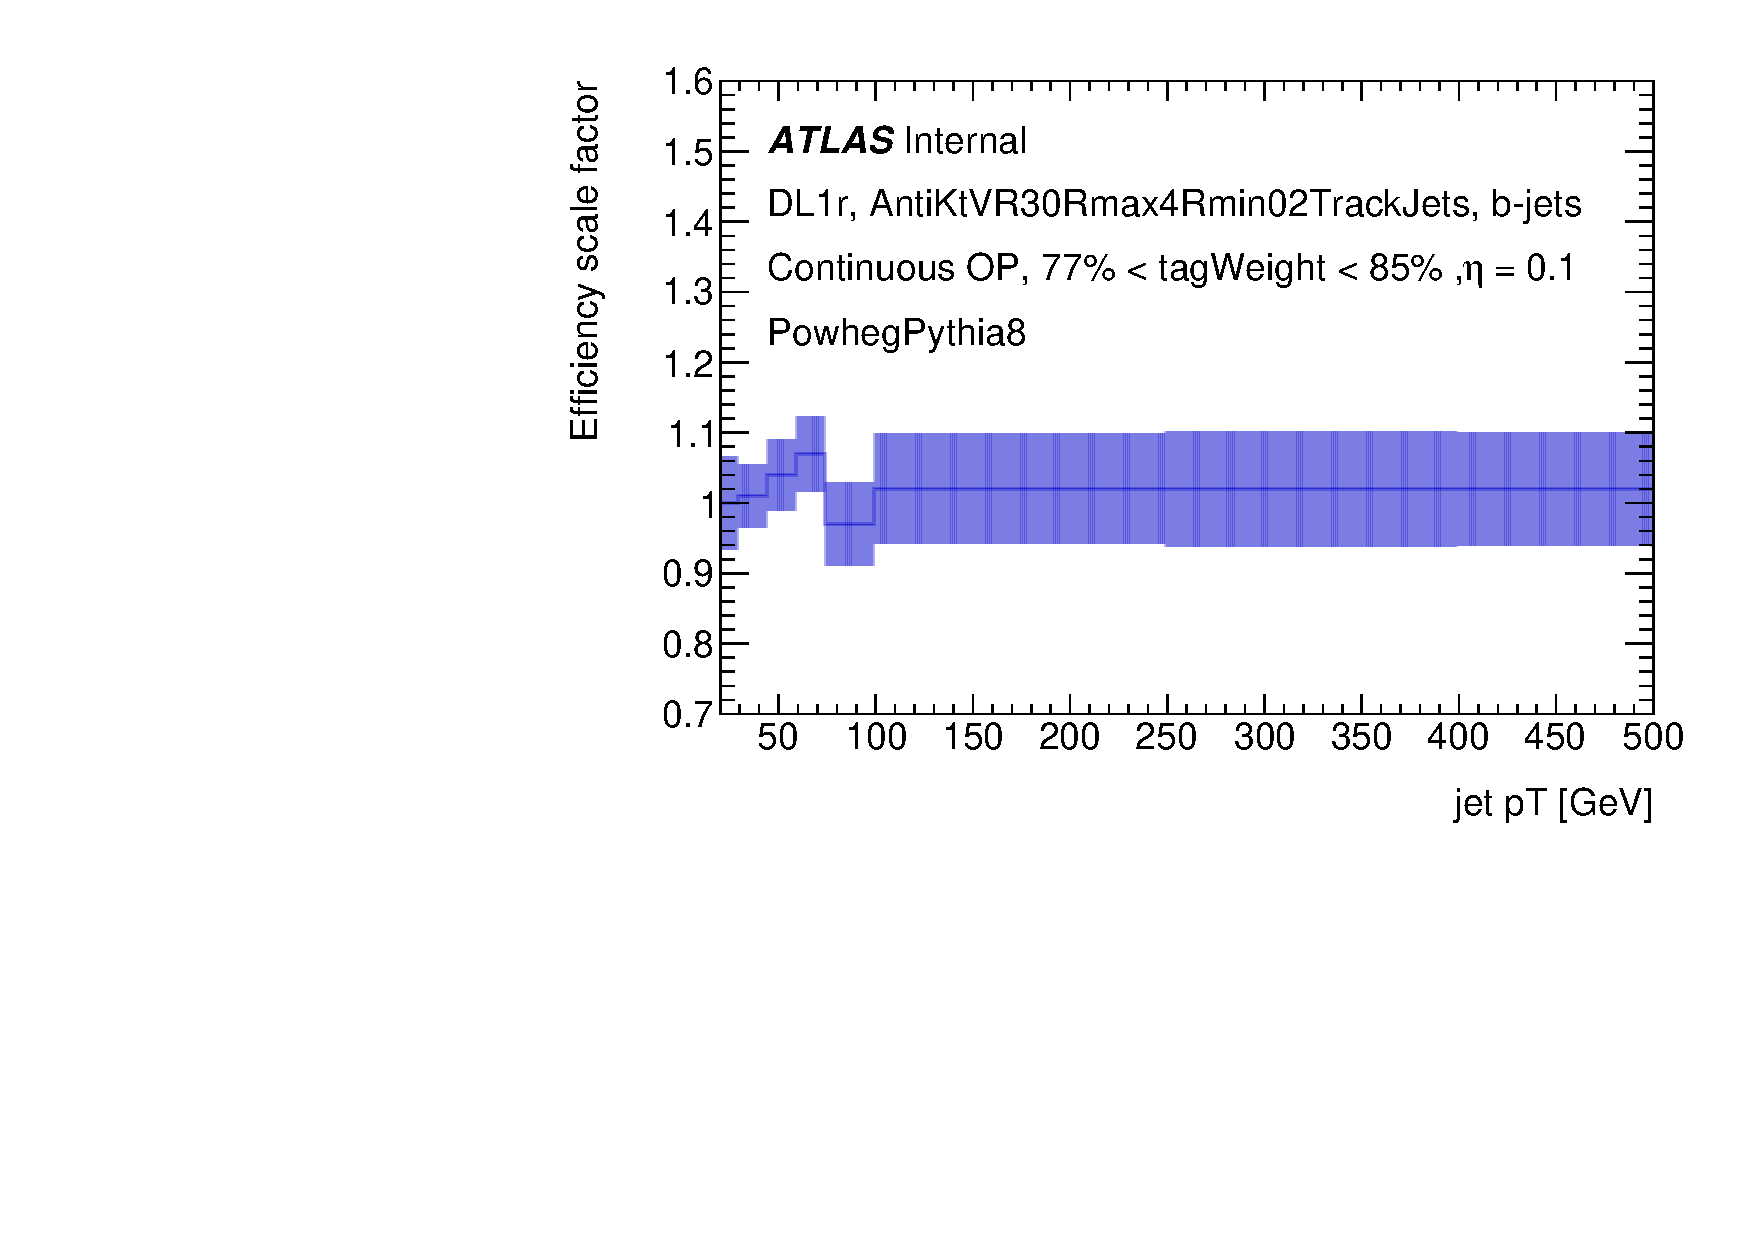
\includegraphics[width=0.48\textwidth]{Images/VH/Obj/FTAGCalib/ftagboo/DL1r_AntiKtVR30Rmax4Rmin02TrackJets_BTagging201903_Continuous_B_410470_77_85_eta01.pdf}
    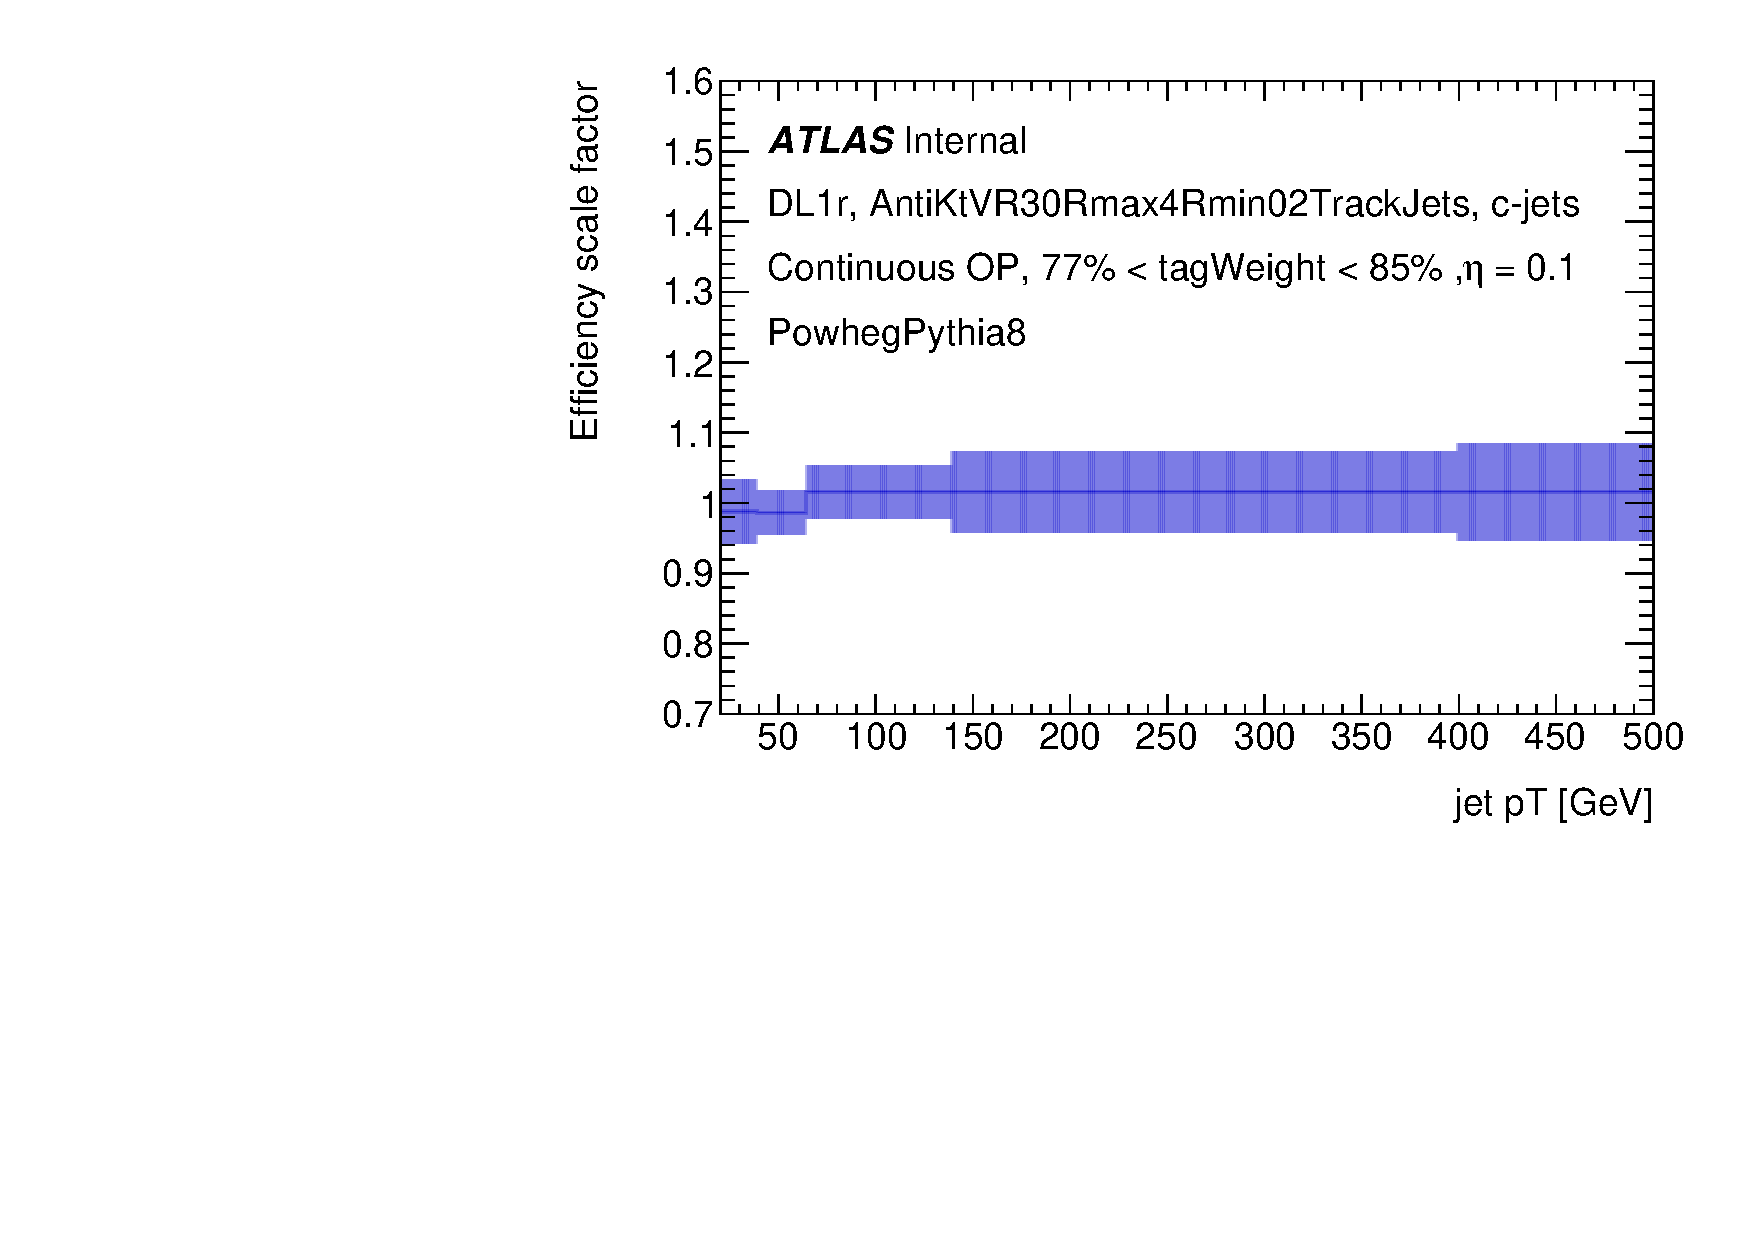
\includegraphics[width=0.48\textwidth]{Images/VH/Obj/FTAGCalib/ftagboo/DL1r_AntiKtVR30Rmax4Rmin02TrackJets_BTagging201903_Continuous_C_410470_77_85_eta01.pdf}
    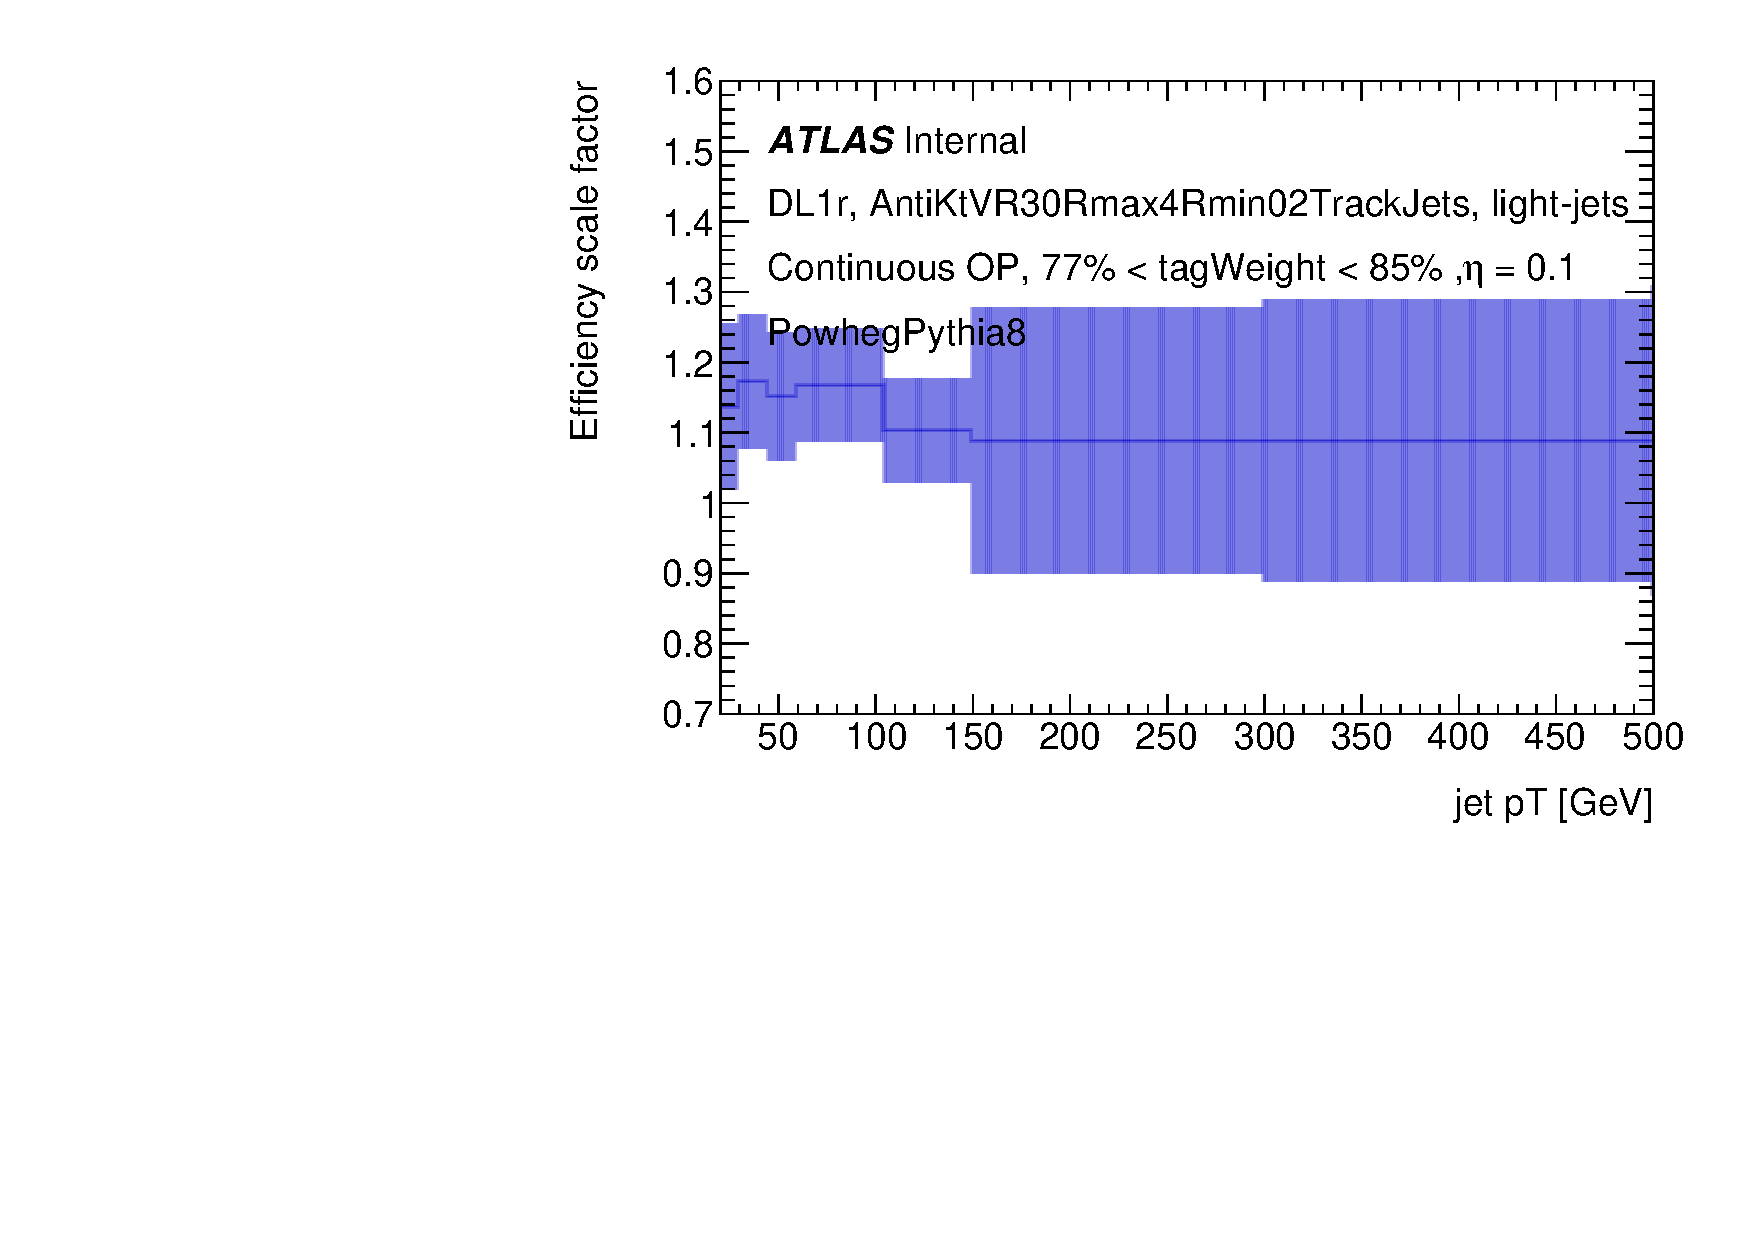
\includegraphics[width=0.48\textwidth]{Images/VH/Obj/FTAGCalib/ftagboo/DL1r_AntiKtVR30Rmax4Rmin02TrackJets_BTagging201903_Continuous_Light_410470_77_85_eta01.pdf}
    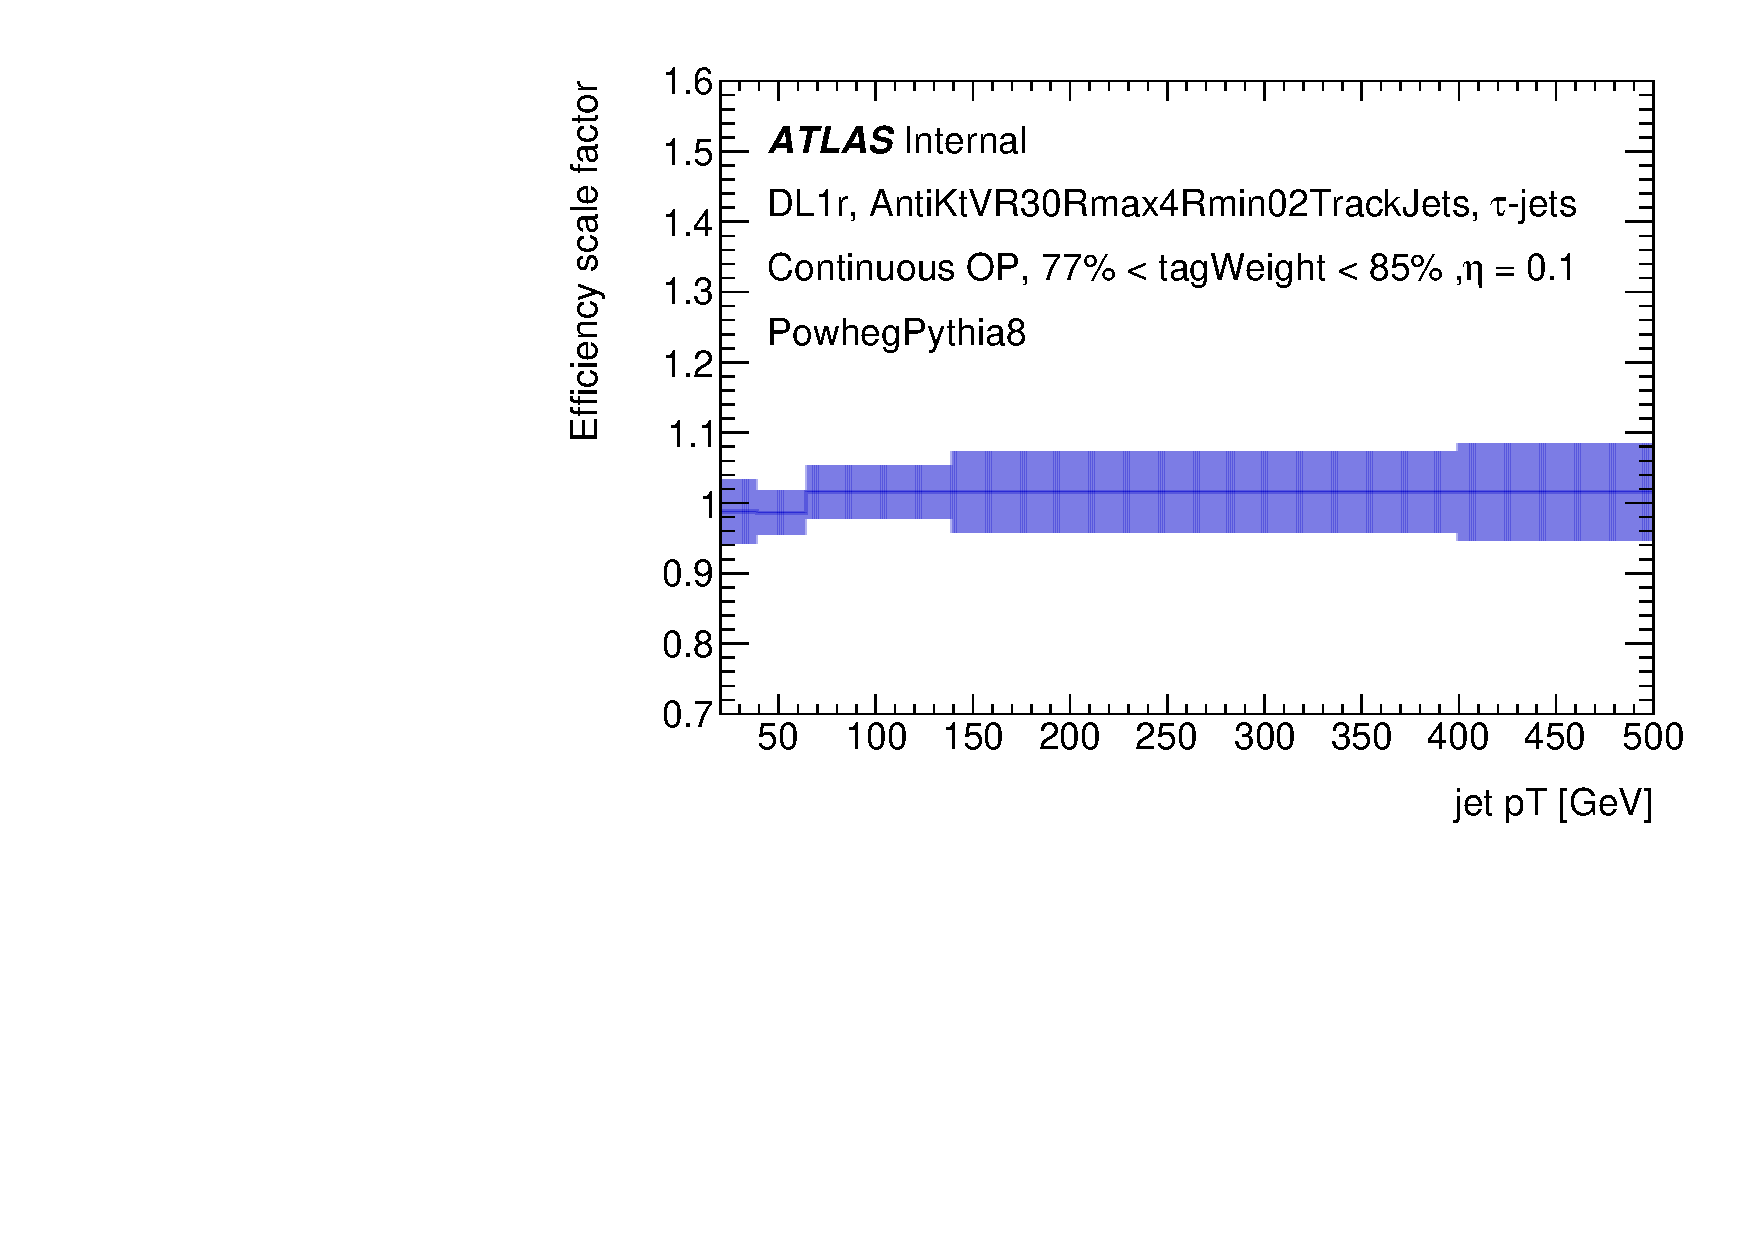
\includegraphics[width=0.48\textwidth]{Images/VH/Obj/FTAGCalib/ftagboo/DL1r_AntiKtVR30Rmax4Rmin02TrackJets_BTagging201903_Continuous_T_410470_77_85_eta01.pdf}
    \caption{ Example of the boosted \vhb\ efficiency scale factor calibration results of the DL1r tagger on PowhegPythia8 \ttb\ samples for the $77\%<\epsilon_j<85\%$ bin. The scale factors of $\tau$-jets are from $c$-jet calibration. From the internal documentation.}
    \label{appfig:FTAG_calibration_boosted}
\end{figure}


\clearpage
\section{Analysis Categorisation}\label{ap-vhCat}
This section offers more details in two elements of the categorisation in the resolved regime: the $\Delta R$ cut and the resolved top CR for the 0- and 1-lepton channels.

\subsection{The $\Delta R$ Cut Between Higgs Candidate Jets}\label{ap-sec-vh-deltaR}
The angular separation between the two candidate jets $\Delta R(j_1, j_2)$, as defined in Equation \ref{eq-deltaR}, can be used to define a control region enriched in $V$+jets and $t\bar{t}$ backgrounds since these two processes give candidate jets with a flat angular spectrum while the signal peaks at low values of $\Delta R$. A \textit{high $\Delta R$} control region (High $\Delta R$ CR) is defined using parametrised cuts on $\Delta R$ between the Higgs candidate jets as a function of $p_T^V$. An additional \textit{low $\Delta R$} control region (Low $\Delta R$ CR) for the 1L channel in the resolved \vhb\ is also introduced (for \vhc, it is merged with the signal region). The philosophy behind the parametrisation of this function is to adapt the cut on the expected angular separation between the two Higgs candidate jets as a function of how boosted they are, as described by the $p_T^V$ variable. For signal events, we expect the $H$ and $V$ to be approximately back-to-back hence $p_T^V$ is a good proxy for $p_T^H$ while benefiting from better experimental resolution, as it is reconstructed from leptons $p_T$ and/or $E_T$, depending on the channel. From physical principals, boosted candidate jets are indeed expected to have a lower angular separation. The cuts are defined by fitting a template function $ c_1 \times e^{c_2 + c_3 \times p_T^V}$ to the \vhb\ selected events, so that:   
\begin{itemize}
\item 95\% (85\%) of the \vhb\ signal is below the top limit for the 2-jet (3-jet) signal region,
\item 90\% of the diboson process is above the bottom limit in both signal regions.
\end{itemize}

The results of these fits for the 1L channel are displayed in Figure~\ref{fig:drccptvCutsVHcc}, showing the signal yield in a 2-dimensional histogram ($p_T^V$ vs $\Delta R_{c\bar{c}}$) for different tags applied. Cuts derived on the \vhc\ selected events showed good agreement with the \vhb\ derived cuts. The $VH(H\rightarrow b\bar{b})$ cuts is chosen so that the kinematic selection of the two analyses is harmonised. \\

\subsection{Resolved Top Control Region in 0L and 1L}
The top control region (topCR) is used to constrain the rather significant top background that peaks at signal-like values of the discriminant variables. Indeed, when the candidate jets selected correspond to the $b$- and $c$-jet from a $t\bar{t}$ decay, the invariant mass of the pair peaks at 120 GeV, exactly the region of interest for a Higgs decay search. The topCR is defined by requiring at least one $c$-tagged jet in combination with at least one $b$-tagged jet using the \textit{AllSignal} strategy, as previously described. This tagging requirement renders it orthogonal to the signal region of the analysis and targets the decay topology of the different top processes: 
\begin{itemize}
\item Semi-leptonic $t\bar{t}$ decay: both $t$ follow the usual decay chain  $t \rightarrow b$ + $W$, with one of the $W$ decaying leptonically and the other one to a pair of quarks. Some events from this process can enter the signal region when some quarks are $c$-tagged or if the $b$-jets are mis-tagged or flew out of the detector acceptance. Requiring the combination of a $b$-tag and a $c$-tag effectively selects this process, the $b$ coming from the direct $t$ decay and the $c$ from a subsequent $W$ decay. 
\item Single top $t$-quark: predominantly the $Wt$ process $W$ $t \rightarrow W$ +  $b$ + $W$, with one $W$ decaying leptonically and the other hadronically. Some of these background events can enter the signal region if the $b$- is missed and if a jet is $c$-tagged, from the extra $W$ or if the $b$-jet is mis-tagged. Events from the single-top $t$- and $s$-channel of the process $t \rightarrow b$ + $W$ bring a smaller contribution, as the $c$-tagged jet must come from \textit{Initial State Radiation} (ISR) or \textit{Final State Radiation} (FSR) if the $b$ is not mis-tagged. Single-top is a minor background in 0L and 1L, with the main component being the production of $Wt$ pairs. The $t$-channel and $s$-channel contribute less than 1\% of the total background.
\end{itemize}

Of the two processes, the $t\bar{t}$ is therefore the most important one and a main background in the 0L and 1L channels. Due to their similarities, the $t\bar{t}$ and $Wt$ processes are considered as a single \textit{top} background in the analysis. In 2L, because this top background is small, no flavour-based topCRs are introduced and a different strategy is employed where the top is directly constrained in a pure top-$e\mu$ control region defined by requiring two charged leptons of different flavours. For the 0L and 1L channels, the expected top background normalisation and its kinematic distributions, as given by the MC simulation, are adjusted using data in the topCRs; this is extrapolated to the signal regions under consideration of extrapolation effects (and corresponding extrapolation uncertainties) that account for differences between the topCRs and SRs. \\

The combined top background is separated into different components, depending on the true flavour of the two candidate jets, that can be combined during the statistical analysis. These are:
\begin{itemize}
\item top($bb$): in this case, the two $b$-jets produced during the $t\bar{t}$ decay are selected. This is a small component in the signal regions of the $VH(H\rightarrow c\bar{c})$ analysis, due to the 70\% efficiency WP for $b$-tagging and the low mis-tag rate for $b$-jets in $c$-tagging. Naturally, in $VH(H\rightarrow b\bar{b})$ it is the leading contribution. Due to the origin of the candidate jets, a large $\Delta R_{b\bar{b}}$ is expected between the two $b$-jets so this component is most effectively constrained by the High $\Delta R$ CR. 
\item top($bc$): where the $b$ is from a $t$ decay and the $c$ from a subsequent $W$ hadronic decay (or from ISR/FSR though this is less likely). Given the definition of the topCR, this is the dominating component in that region and the most important to constrain in the signal regions of the $VH(H\rightarrow b\bar{b}/c\bar{c})$ analyses due to its signal-like kinematics. 
\item top($bl$): where $l$ stands for anything not $b$ nor $c$ (light jets predominantly but also some mis-tagged hadronic $\tau$). This component is similar to the top($bc$) as it also consists of a $b$ + a jet from the $W$ and can end up in the SRs and topCRs due to mis-tags.
\item top($lq$): where $l$ is as above and $q$ can be any sort of jet except a $b$. This is a small component that mostly accumulates in the background-like part of the BDT score distribution. It is not constrained in the high $\Delta R$ regions nor the topCRs.
\end{itemize}
The signal region distributions in the 1L channel in the $p_T^V$ range $[150, 250]$ GeV are displayed in Section \ref{appsec-vh-analRegPosfit} of the Appendix. While the top is not the dominant background, except in the tighter tagged TT 3-jet region, its relative contribution to the background composition increases at signal-like values of the discriminant. \\

The components contributing the most in the \vhc\ side of the analysis are the top($bc$) and top($bl$), due to the tagging requirement. There is very little top($bb$) thanks to the good performance of the tagger. Top($lq$) is mostly found in the looser tag regions (NT, LT) and not where the signal peaks. The philosophy behind the design of the top CR leverages the pseudo-continuous tagging to select the highest $p_T$ $b$-tagged and $c$-tagged jets as Higgs candidates. Thus, BL and BT regions are defined depending on whether the highest $p_T$ $c$-tagged jet is loose- or tight-tagged. The regions are further split in the number of jets and the same definition is used in the 0L channel. The full tag compositions of each region are as follows:

\begin{itemize}
\item 2-jet: \quad BL: $BL$;  \quad BT: $BT$
\item 3-jet: \quad BL: $BLN$, $BLL$;  \quad BT: $BTN$, $BTL$, $BTT$, and $BBT$
\end{itemize}
In the \textit{AllSignal} strategy, the Higgs candidates in the topCR are always the highest $p_T$ $b$- and $c$-tagged jets. This selection was observed to make the top control region distributions more closely match the distributions in the signal regions. For the fit, only the $BT$ region is used, as it provides sufficient control on the important top background components. The $BL$ region is only used to validate the, assessing the data-\gls{mc} agreement after correcting the yields of the major backgrounds, as is shown in Figure \ref{fig:val_BLtopCR}. \\


For $VH(H\rightarrow c\bar{c})$, the $bc$ and $bl$ components are the most important to constrain. In $VH(H\rightarrow b\bar{b})$, while the $bc$ component is also significant and can benefit from the topCRs, the most important contribution comes from the $bb$ one and is well constrained by the High $\Delta R$ CR, since in a $t\bar{t}$ decay the two produced $b$-jets tend to be separated by a large $\Delta R$ due to the event topology. For the Combined Analysis, the SRs and CRs of both analyses are considered simultaneously. The High $\Delta R$ CR from \vhb\ are used to constrained the residual top$(bb)$ component in \vhc. \\

\newpage
\subsection{Truth Tagging}\label{app-truth-tagging}
The tagging method described in Section \ref{sec-selectionandcat}, referred to as \textit{direct tagging}, is a cut-based method where a jet passes or fails a threshold cut, as defined by dedicated working points in the \gls{pcft} or PCBT schemes. These \gls{wp} have a large rejection for $b$-tagging due to the good performance of the method. For $c$-jets, the tagging efficiency is low and many $c$-jets end up rejected by the selection. This problem is compounded by the event selection criteria, requiring two $b$-tags or at least one tight $c$-tag to enter the analysis' regions. Only a part of the events in the simulated samples satisfy these requirements, and most are discarded from the analysis. Having sufficient \gls{mc} statistics in all regions is essential to effectively model the backgrounds and reduce the \gls{mc} statistical uncertainty. An alternative approach to direct tagging used in the analysis to retain the large \gls{mc} statistics is \textit{truth tagging}. Rather than applying a pass-fail decision, truth tagging reweighs events by their probability of being selected at a specific working point, based on truth information only available in the simulated samples. The tagging scale factors are applied in the analysis after truth tagging. \\

Mathematically, truth tagging derives a per event weight $w$ from the tagging efficiency $\epsilon_j(\textbf{x}, \theta)$ for a given flavour jet $j$ to be tagged at a given working point of a classifier trained on a set of input variables $\textbf{x}$, with the assumption that the efficiency is parametrisable as a function of several variables $\theta$, such as the jet $p_T$, $\eta$, ... For a set of $m$ jets with a tagged subset $T_i$ of cardinality $|T_i| = n$, and defining the efficiency at tagging the tagged jets as \[\epsilon(T_i,\textbf{x},\theta) = \prod_{j\in T_i} \epsilon_j(\textbf{x},\theta),\] and the efficiency at not tagging the set of untagged jets $\tilde{T}$, with $|\tilde{T}_i| = m-n$, \[ \epsilon_{in}(\tilde{T}_i,\textbf{x}, \theta) = \prod_{j\in \tilde{T}_i} (1-\epsilon_j(\textbf{x}, \theta)),\] the expression for $w$ can be factorised as \cite{ATL-PHYS-PUB-2022-041}: 

\begin{equation}
  \label{eq:truthtagging1}
      w = \sum_i^C \epsilon(T_i,\textbf{x},\theta)\cdot \epsilon_{in}(\tilde{T}_i,\textbf{x},\theta),
  \end{equation}
where the sum is over all possible permutations of tags $C$. The probability of a specific configuration $i$ is given by \[ P_i = \frac{ \epsilon(T_i,\textbf{x},\theta)\cdot \epsilon_{in}(\tilde{T}_i,\textbf{x},\theta)}{w}.\] When deploying the technique, one possible permutation is randomly sampled to keep distinct bins uncorrelated in the fit and the whole weight $w$ is applied to it. \\

Technically, truth tagging was deployed with map-based 2D histograms $p_T - \eta$ parametrising the tagging efficiency of the jets in the latest standalone \vhb\ and \vhc\ analysis \cite{ATLAS:2020fcp, Collaboration:2721696}. Such histograms are called \textit{efficiency map}, leading to the implementation being referred to \textit{map-based truth tagging}. These maps were derived individually for each $b$-, $c$-, light-, and $\tau$-jets flavour and each working point. A further possibility is to combine direct tagging with truth tagging into the so-called \textit{hybrid tagging} strategy, in which a portion of the events are direct tagged and the rest is truth tagged. This last approach limits the mis-modelling incurred by truth tagging and remove the need to correct for non-closure effects. \\

A new approach considered for the combined analysis relies on a \gls{gnn} to perform the so-called \textit{GNN truth tagging} \cite{ATL-PHYS-PUB-2022-041}. This removes the statistical dispersion limitation of high-dimension efficiency maps. Interestingly, it also becomes possible to include more variables to parametrise the efficiency, leading to better agreement with the direct tagging distribution comparing to map-based truth tagging. The network builds a fully-connected graph with several layers message-passing updates \cite{graphInductiveBias}, where each node represents a jet in the event\footnote{Only central jets in the resolved regime and track-jets associated with the large-$R$ jet in the boosted regime.}. The features per node are the jet-level and event-level variables listed in Table~\ref{tbl:gnn-features}, with the angular separation between the jets set as edge between the nodes. Finally, a fully-connected \gls{nn} receives the last update graph and outputs all track-jets or jets flavour-tagging efficiencies.

\begin{table}[tbp]
  \begin{center}
      \begin{tabular}{C{8cm}C{5cm}} \hline \hline
        Jet features & Type of variable \\ 
        \hline
        Jet $p_T$ & \\
        Jet $\eta$ & \\
        Jet $\phi$ & \\
        Jet flavour label & Jet level feature \\
        Mass of $p_T$ leading b or c hadron in the jet $\phi$ & \\
        $p_T$ of $p_T$ leading b or c hadron in the jet $\phi$ & \\
        $\eta$ of $p_T$ leading b or c hadron in the jet $\phi$ & \\
        $\phi$ of $p_T$ leading b or c hadron in the jet $\phi$ & \\
        \hline
        Average number of interactions per event $\langle \mu \rangle$ & Event level variable\\
        \hline
        Angular separation between two jets $\Delta R$ & Jet-pair variable\\
        \hline \hline
      \end{tabular}
    \caption{The input features to parametrise the efficiency in GNN truth tagging.}
    \label{tbl:gnn-features}
  \end{center}
\end{table}

In the combined analysis, truth tagging is deployed in all regimes and trained independently for samples with different \gls{mc} generators\footnote{Since the \glsfirst{sf} are derived per generator.}, inclusively in all lepton channels. In the resolved regime, the training is further separated for each background samples. The GNN truth tagging is seen to improve the parametrisation of the efficiency, showing better closure with the direct-tagged distributions than the map-based approach. However, some unclosure remain for particular flavours. To limit this effect, hybrid tagging is also deployed in the combined analysis with GNN truth tagging. In this hybrid tagging, $b$-jets are direct tagged and other jets are GNN truth tagged in the resolved regime. In the boosted regime, all jets are truth tagged due to the limited \gls{mc} statistics. The strategies deployed in the different regimes of the analysis are summarised in Table \ref{tbl:gnn-strategy}.

\begin{table}[!htbp]
  \begin{center}
      \begin{tabular}{c|c|c|c} \hline \hline
        & \vhb\ Resolved & \vhc\ & \vhb\ Boosted\\ 
        \hline
        Hybrid tagging & Yes ($b$-jets are DT) & No (fully TT) & No (fully TT)  \\
        Truth tag \gls{wp} & 70\% $b$ \& 70\% $b$ & $c$-tight \& $c$-tight & 85\% $b$ \& 85\% $b$ \\
        MC stat. \% for TT regions & 100\% & 8\% & 100\%\\
        \hline
        $V+$jets & HT & TT & TT\\
        single-top $s/t$ & HT & TT & TT\\
        single-top $Wt$ & DT & DT & TT\\
        \ttb\ & DT & DT & TT\\
        diboson & DT & DT & TT\\
        signal & DT & DT & DT\\
        \hline \hline
      \end{tabular}
    \caption{The tagging strategies to be used in the different regimes of the analysis, with truth tagging (TT), direct tagging (DT), and hybrid tagging (HT).}
    \label{tbl:gnn-strategy}
  \end{center}
\end{table}

The tagging strategy is optimised to maximise the \gls{mc} statistics of the different regions and boost the sensitivity. Truth and hybrid tagging are only deployed when they deliver a meaningful improvement to the analysis. The full tagging strategy of the analysis is:
\begin{itemize}
  \item Resolved \vhb: direct tagging is used except for the $V+$jets and single-top $s/t$ process where hybrid tagging is deployed, with both $b$-jets being direct tagged at the 70\% \gls{wp}.
  \item \vhc: similar to the resolved \vhb, with the $V+$jets and single-top $s/t$ now fully GNN truth tagged. For \vhc, the samples are split based on the tag region to avoid reusing an event twice. For example, an initially $LN$ direct-tagged event could enter the $TT$ region with a low truth tag weight, thereby removing the statistical independence assumed between \gls{mc} events. To correct this, only 8\% of the \gls{mc} statistics is randomly sampled and truth tagged to the $TT$-tag region, and the rest is passed to direct tagging (for the $TL$, $NT$, $LN$, and $BT$ tags). 
  \item Boosted \vhb: GNN truth tagging is applied for all background except the signal samples that are direct tagged.
\end{itemize}
Unfortunately, at the time of writing this thesis the analysis samples were not yet fully updated to the tagging scheme described here. Instead, the resolved \vhbc\ all use direct tagging everywhere and the boosted regime uses full GNN truth tagging. Moving to the full tagging scheme outlined above should have a small positive effect on \gls{mc} statistics uncertainty and bring smoother \gls{mc} templates, reducing the noise in the fit.
% TODO: this is not true: the main note was including this only for truth tagging, not for the rest: The above outlined strategy outlines the final strategy. The plots and yield tables - and correspondingly fit results - do not reflect this strategy yet and instead direct tagging is used for resolved \vhbb and \vhcc regimes and full GNN truth tagging for the boosted \vhbb regime, since fit inputs were not ready in time for this version of the note. The expected differences on the sensitivity are small (small decrease in the impact of MC stat. uncertainty and smoother MC templates that will make the fit less prone to statistical ``noise'' making the fit more robust.)}

To showcase the effectiveness of the method, the direct tagged, GNN truth tagged, and map-based truth tagged $m_{cc}$ distributions of the \textsc{Sherpa} 2.2.11 simulated $W+$jets in the 1-lepton 2-jet CRHigh \ptv\ $\in [250, 400]$ GeV region of the \vhc\ is displayed in Figure \ref{fig:truthtaggingW1LVHcc}. The GNN truth tagging is found to be in better agreement with the direct tagged distributions in the regions of sufficient statistics. In the $W+l$ region, direct tagging leads to statistically depleted regions with large uncertainties: this is effectively corrected by the GNN-based truth tagging approach. No significant non-closures are observed for from GNN truth tagging with the outlined strategy.

\begin{figure}[h!]
  \begin{subfigure}[b]{0.32\textwidth}
    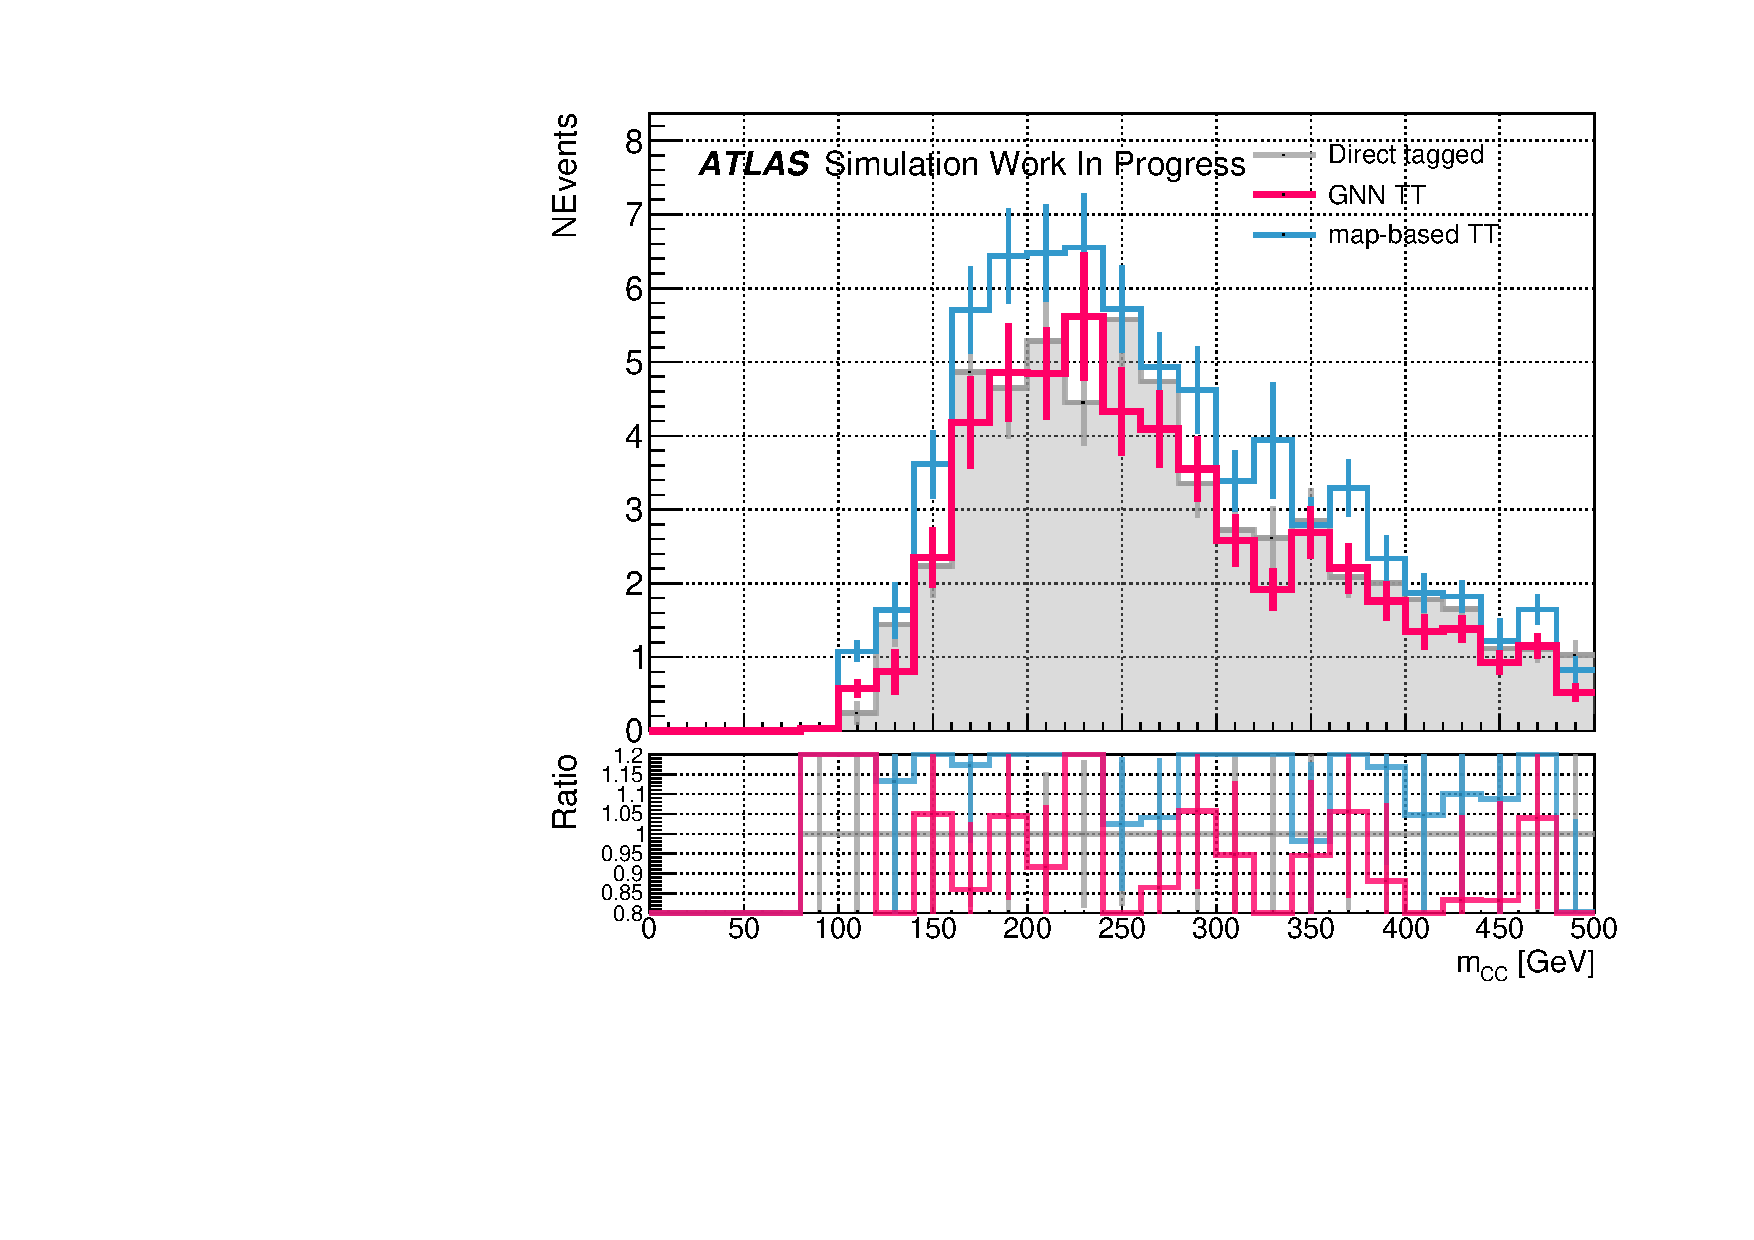
\includegraphics[width=\textwidth]{Images/VH/Tagging/Whf_2tttag2jet_250_400ptv_CRHigh_mCC.pdf}
  \caption{$W+$hf in CRHigh.} 
  \end{subfigure}
  \begin{subfigure}[b]{0.32\textwidth}
    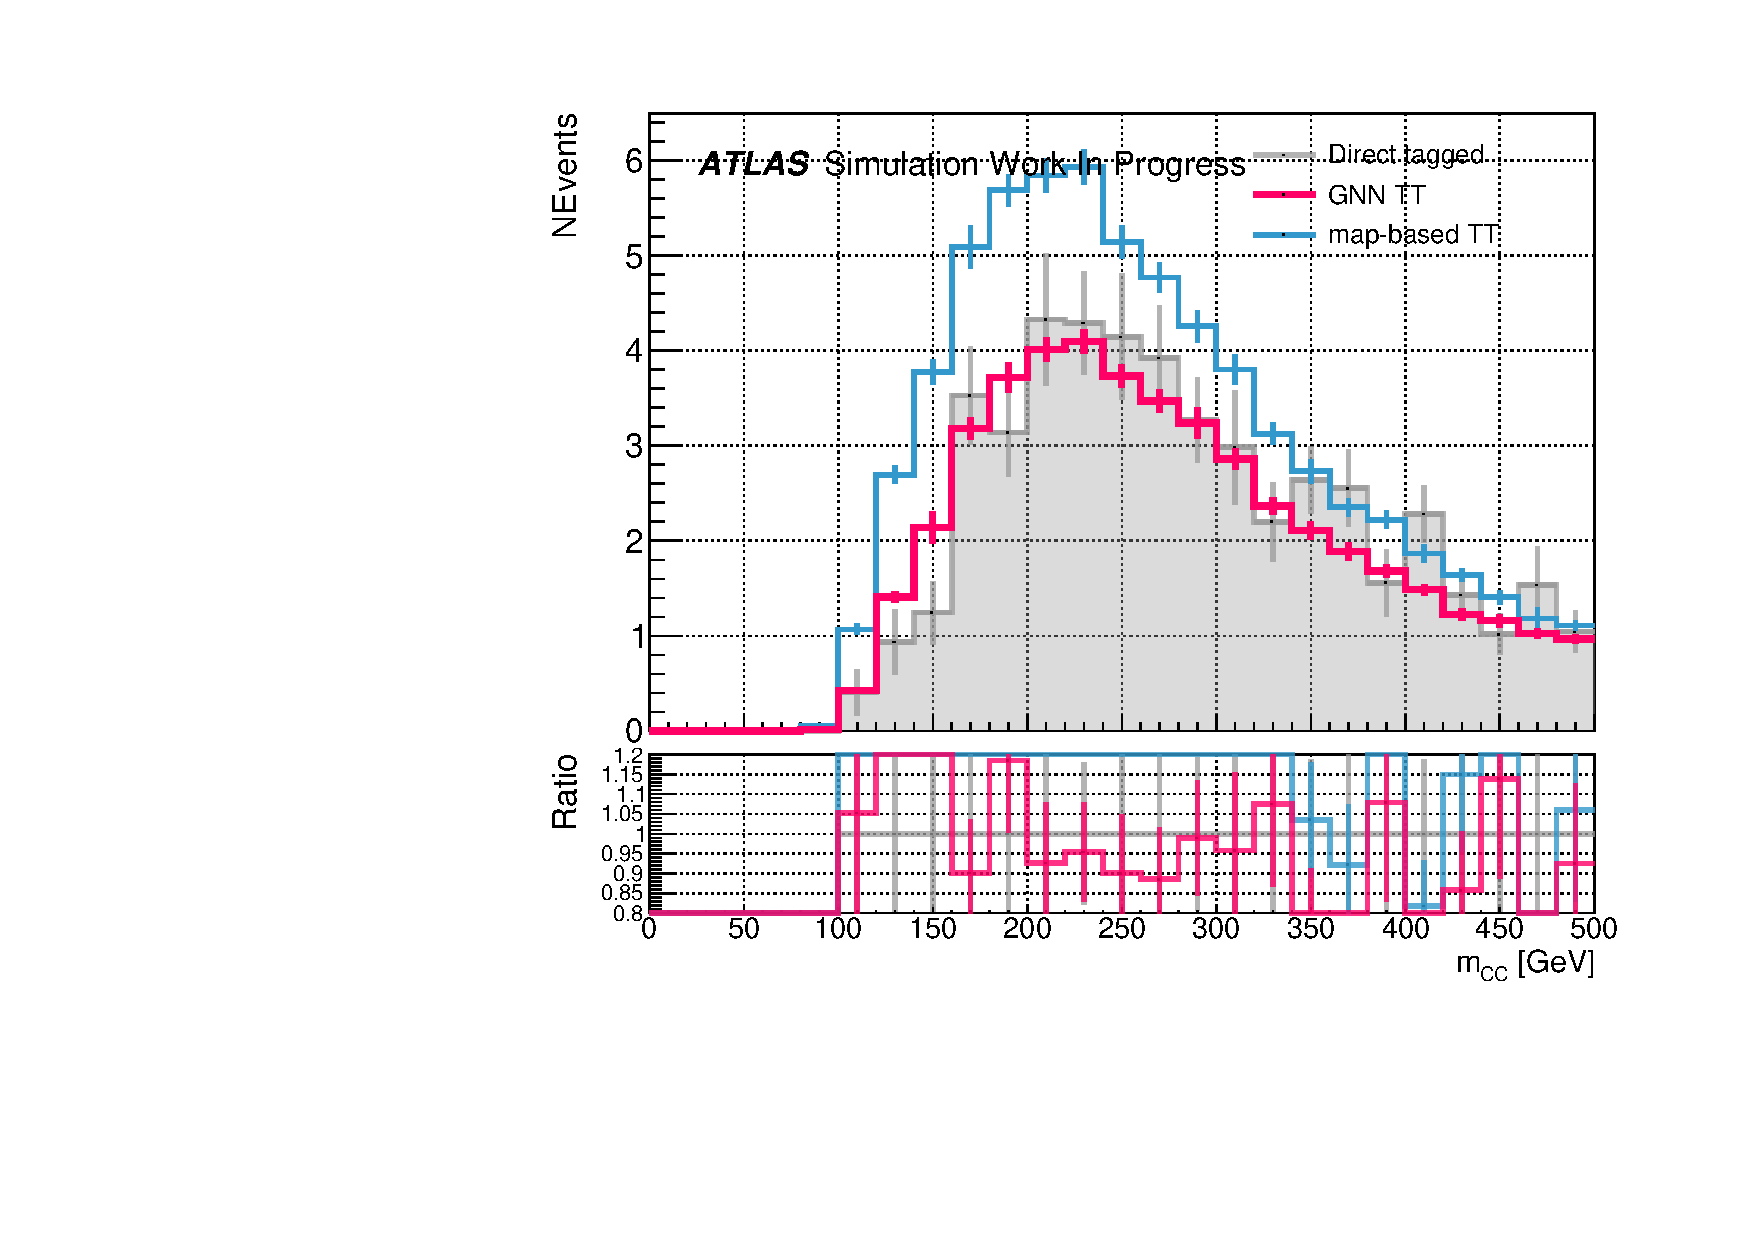
\includegraphics[width=\textwidth]{Images/VH/Tagging/Wmf_2tttag2jet_250_400ptv_CRHigh_mCC.pdf}
    \caption{$W+$mf in CRHigh.}
  \end{subfigure}
  \begin{subfigure}[b]{0.32\textwidth}
    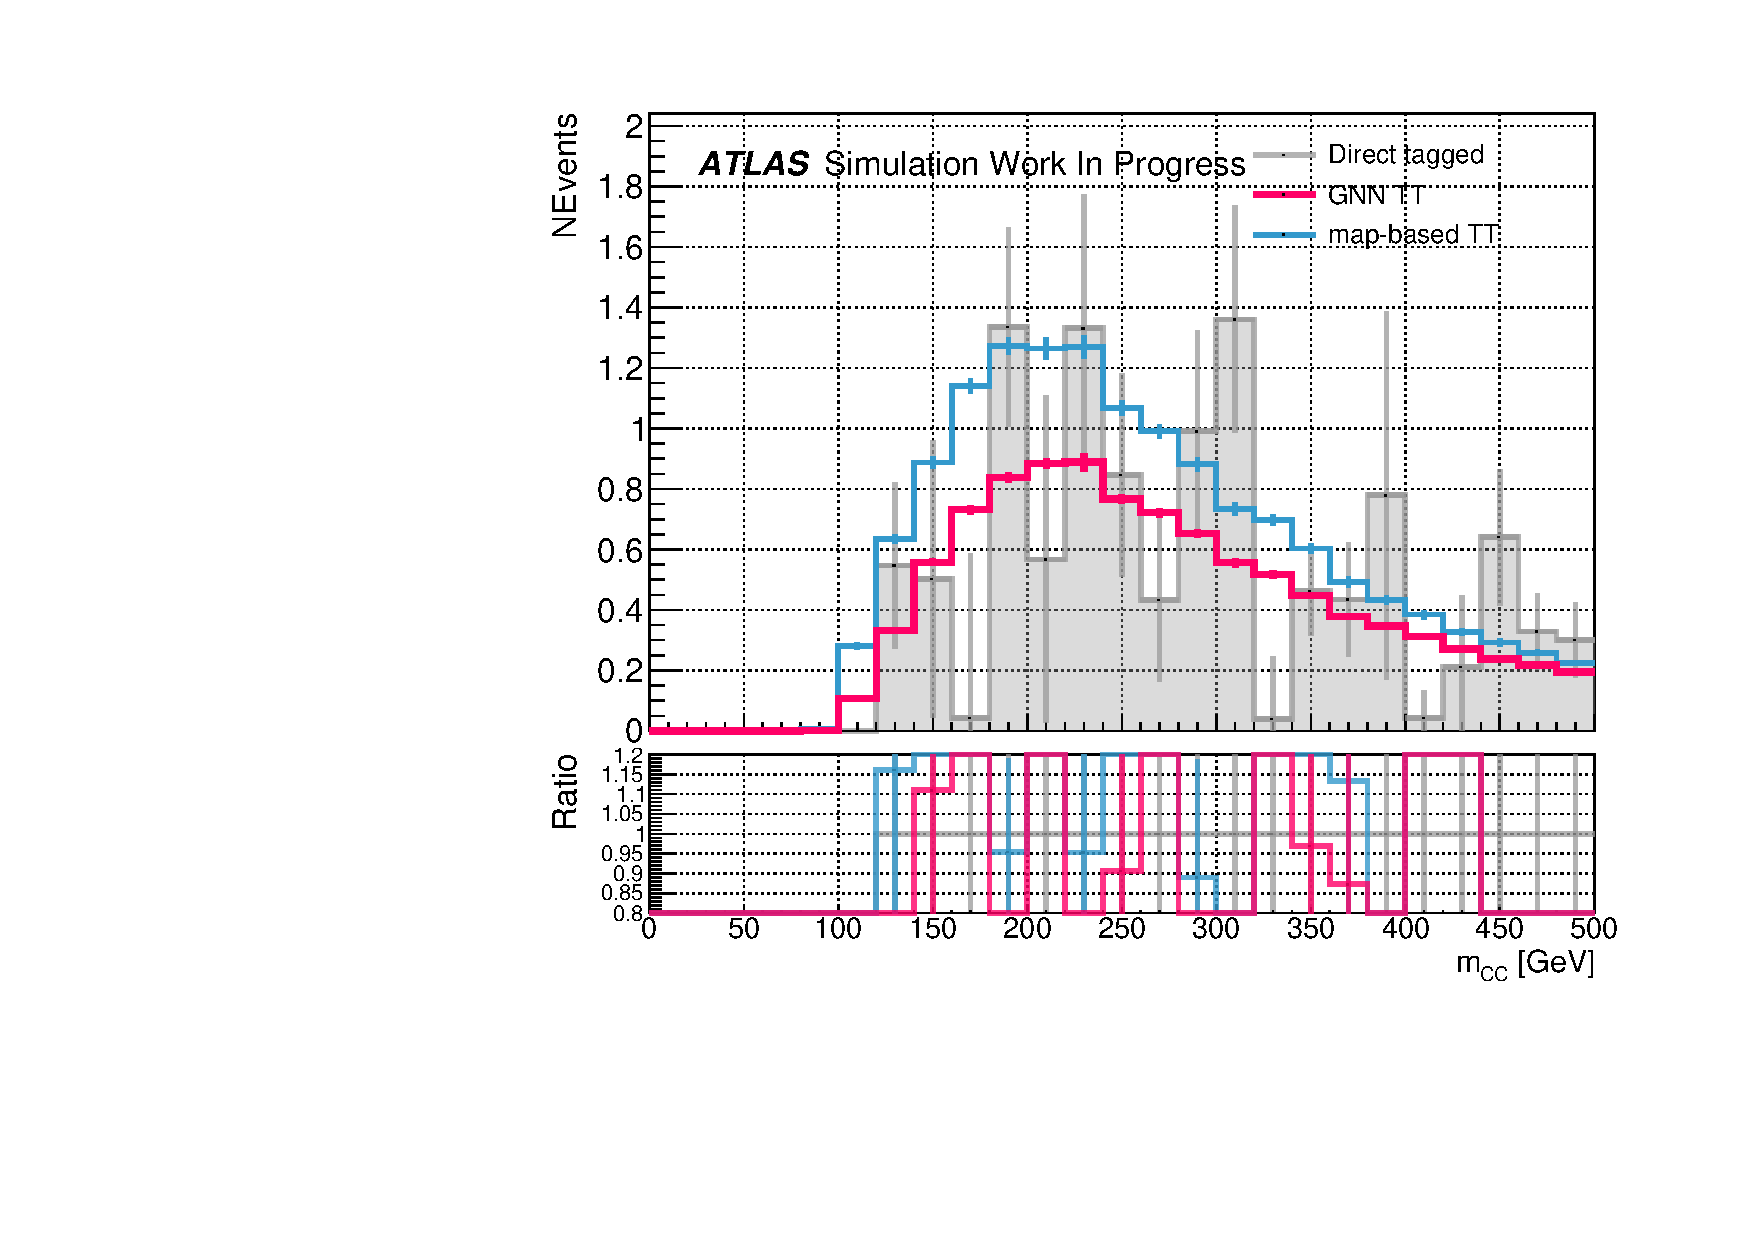
\includegraphics[width=\textwidth]{Images/VH/Tagging/Wl_2tttag2jet_250_400ptv_CRHigh_mCC.pdf}
    \caption{$W+l$ in CRHigh.}
  \end{subfigure}
  \caption{Comparing the tagged $m_{cc}$ distribution for the \vhc\ of the \textsc{Sherpa} 2.2.11 simulated $W+$jets in 1L CRHigh 2-jet region, in the 250 GeV $<$ \ptv\ $< 400$ GeV region. TT stands for truth tagging.}
  \label{fig:truthtaggingW1LVHcc}
\end{figure} 

\clearpage
\section{MVA Variables}\label{ap-MVA}
This section is dedicated to the set of variables used to train the various MVAs used in the analysis. Notice that the $H$ candidate is reconstructed by the selected jets sorted by \pt\ and labelled $j_1$ and $j_2$.

\paragraph{Input variables for the resolved regime:}
\begin{itemize}
    \item \ptv: transverse energy of the vector boson. In 0-lepton channel it is equivalent to the missing transverse energy ($E_T^{\textrm{miss}}$); in 1-lepton channel it is the vector sum of $E_T^{\textrm{miss}}$ and the lepton \pt; in 2-lepton channel, it is the vector sum of the 2 charged lepton \pt.
    \item $p_{\text{T}}^{j_1}$ and $p_{\text{T}}^{j_2}$: transverse momenta of the Higgs candidate jets. $j_1$ refers to the jet with higher \pt.
    \item $m_{j_1j_2}$ or $m_J$: invariant mass of the reconstructed $H$ system, depending on the analysis regime.
    \item $\Delta R (j_1,j_2)$: angular distance between the two Higgs-candidate jets, defined as $\Delta R(i,j) = \sqrt{(\Delta\phi(i,j))^2+ (\Delta\eta (i,j))^2}$ with $\Delta\phi(i,j) = \phi_i-\phi_j$ the azimuthal and $\Delta \eta(i,j)= \eta_i-\eta_j$ the pseudorapidity distances.
    \item $m_{j_1 j_2 j_3}$: invariant mass of two Higgs-candidate jets and the remaining jet with highest \pt. When there are only 2 jets in an event, $m_{j_1 j_2 j_3}=m_{j_1j_2}$.
    \item $\Delta \phi(\textbf{$V$},\textbf{$H$})$: azimuthal distance between the reconstructed vector boson $V$ and Higgs boson candidates $H$.
    \item $\mathrm{bin}_{\mathrm{DL1r}(j1)}$, $\mathrm{bin}_{\mathrm{DL1r}(j2)}$: variable showing the tagged-bin the jet or track-jet $j_1$ belongs to (5 possible bins, as defined in Section \ref{sec-selectionandcat}) - the untagged $N$, the loose (70\% WP) and the tight (60\% WP) $b$-tagged, and the loose and the tight $c$-tagged bins. In the MVA, the value of the two Higgs-candidate jets or track-jets are used.
    \item $\sum\limits_{i\neq 1, 2}p_T^{j_i}$:\pt~sum of non~$H$ candidate jets that have $p_T>20~\text{GeV}$.
    \item \textbf{0-lepton channel variables}: 
    \begin{itemize}
        \item $|\Delta \eta (j_1,j_2)|$: absolute value of the pseudorapidity distances between the two Higgs-candidate jets or track-jets.
        \item $\min\{\Delta R(j_i, j)\}_{i=1,2}$: the distance in $R$ between the closest $b$- or $c$-tagged Higgs candidate jet and an additional jet with \ptv$>20~\text{GeV}$.
        \item $m_{\textrm{eff}}$: the scalar sum of the \pt of all small-$R$ jets and $E_T^{\textrm{miss}}$ in the event.
    \end{itemize}
    \item \textbf{1-lepton channel variables}:  
    \begin{itemize}
        \item $m_T^W$: transverse mass of the $W$ boson candidate reconstructed from the lepton and $E_T^{\textrm{miss}}$, as presented in the 1L-specific selection of Section \ref{subsubsec-0Lsel}.
        \item $E_T^{\textrm{miss}}$: missing transverse energy. 
        \item $\Delta y(\textbf{$V$},\textbf{$H$})$: rapidity difference between the $V$ and $H$.
        \item $\min\left[\Delta\phi(\textbf{$l$},\textbf{$j_i$})\right]_{i=1,2}$: distance in $\phi$ between the lepton and the closest $b$-tagged ($c$-tagged) $H$ candidate jet. 
        \item $m_{\text{top}}$: reconstructed mass of the leptonically decaying top quark. The longitudinal momentum of the neutrino ($p_{z}^{\nu}$) is first reconstructed the mass of the $W$ boson, and selected to minimise the reconstructed $m_{\text{top}}$ with the 2 Higgs candidates.
    \end{itemize}
    \item \textbf{2-lepton channel variables}: 
    \begin{itemize}
        \item $m_{ll}$: invariant mass of the di-leptons system.  
        \item $\cos{\theta(l^-,\textbf{$Z$})}$: $Z$ boson polarisation sensitive angle. 
        \item $E_T^{\textrm{miss}}/\sqrt{S_{\mathrm{T}}}$: the quasi-significance of $E_T^{\textrm{miss}}$ with $S_{\mathrm{T}}$ being the scalar sum of the \pt\ of the leptons and jets in the event.  
        \item $\Delta y(\textbf{$V$},\textbf{$H$})$: rapidity difference between the vector boson and Higgs boson candidates. 
    \end{itemize} 
\end{itemize}

% new variables: stageB - https://indico.cern.ch/event/1254481/contributions/5270035/attachments/2593141/4475547/MVA%20Stage%20B%20Summary%20(1).pdf
% stageA - https://indico.cern.ch/event/1221988/contributions/5184468/attachments/2568369/4428463/22_12_15_MVARetrainingCampaignSummary.pdf

\paragraph{Input variables for the boosted regime:}
\begin{itemize}
  \item $m_J$: leading-$R$ jet mass, the Higgs candidate.
  \item \ptv: same as in the resolved regime.
  \item $p_{T}^{j_1}$, $p_{T}^{j_2}$ and $p_{T}^{j_3}$: transverse momenta of the track-jets inside the $H$ candidate large-$R$ jet, where $j_1$ and $j_2$ are the $b$-tagged sub-jets, and $j_3$ refers to the leading additional jet.
  \item $\Delta R(j_1,\,j_2)$: angular distance between the two $b$-tagged track-jets.  
  \item $N(\text{track-jets in $J$})$: the number of track-jets that are associated to the leading large-$R$ jet. 
  \item $N(\text{add. small $R$-jets})$: the number of additional small-$R$ jets that are not associated to the leading large-$R$ jet, such that $\Delta R (\text{small-$R$ jet, large-$R$ jet}) > 1.0$.  
  \item  $\Delta \phi(\textbf{$V$},\textbf{$H$})$: same as in the resolved regime.
  \item Colour: variable exploitting the difference in colour-flow between gluon splittings and decay from gls{qcd} singlets states. Colour is defined here as \[ \textrm{Colour} = \frac{\theta_{j_1j_3}^2 + \theta_{j_2j_3}^2}{\theta_{j_1j_2}^2},\] where $\theta$ is the angle between the indexed jets, $j_3$ is the leading additional jet, and $j_2$ are the $H$ candidate jets.
  \item $\mathrm{bin}_{\mathrm{DL1r}(j1,\text{trk})}$, $\mathrm{bin}_{\mathrm{DL1r}(j2,\text{trk})}$: corresponds to the tagged-bin the track-jet belongs to (4 possible bins): 
  the 85\%, the 77\%, the 70\% and 60\% $b$-tagging efficiency bins.
  \item \textbf{0-lepton channel specific variables}
  \begin{itemize}
      \item $E_T^{\textrm{miss}}$: missing transverse energy, same as \ptv.
  \end{itemize}
  \item \textbf{1-lepton channel specific variables}
  \begin{itemize}
      \item $\Delta y(\boldsymbol{V},\boldsymbol{H})$: same as in the resolved regime.
      \item $p_T^l$: transverse momentum of the lepton.
      \item $(p_T^{l} - E_T^{\textrm{miss}})/p_T^W$:  proxy for the $p_T$ imbalance of the charged lepton and the neutrino of the $W$-boson.
  \end{itemize}
  \item \textbf{2-lepton channel specific variables}
  \begin{itemize}
      \item $\Delta y(\textbf{$V$},\textbf{$H$})$: same as in the resolved regime.
      \item $\cos{\theta(\textbf{$l^-$},\textbf{Z})}$: same as in the resolved regime.
  \end{itemize}
\end{itemize}

\clearpage
\section{Top Modelling Uncertainties in the Fit}
There are many processes of relevance in a complex analysis such as the \vhbc. These must individually be modelled, with studies of the pulls of the different systematics required to verify the fit correctly accounts for the background's contribution to the analysis. The risk with such a complex fit structure with large numbers of \glspl{np} necessary to model a large variety of effects is to give the fit too much freedom and, in a sense, overfit to the data distributions. To highlight the process, some top-related pulls are shown in Figure \ref{fig:topPull}, with pulls displayed for both top acceptance uncertainties and \gls{carl} shape systematics. Again, there is good agreement for most pulls between the $VH$ and $VZ$ analyses. In the acceptance systematics part, a very large significant pull is observed for the so-called ``\textit{MetTrigTop}'', an \etm\ trigger related experimental uncertainty derived from the top-process, as described in \ref{sec-unc}. 

\begin{figure}[h!]
    \centering
    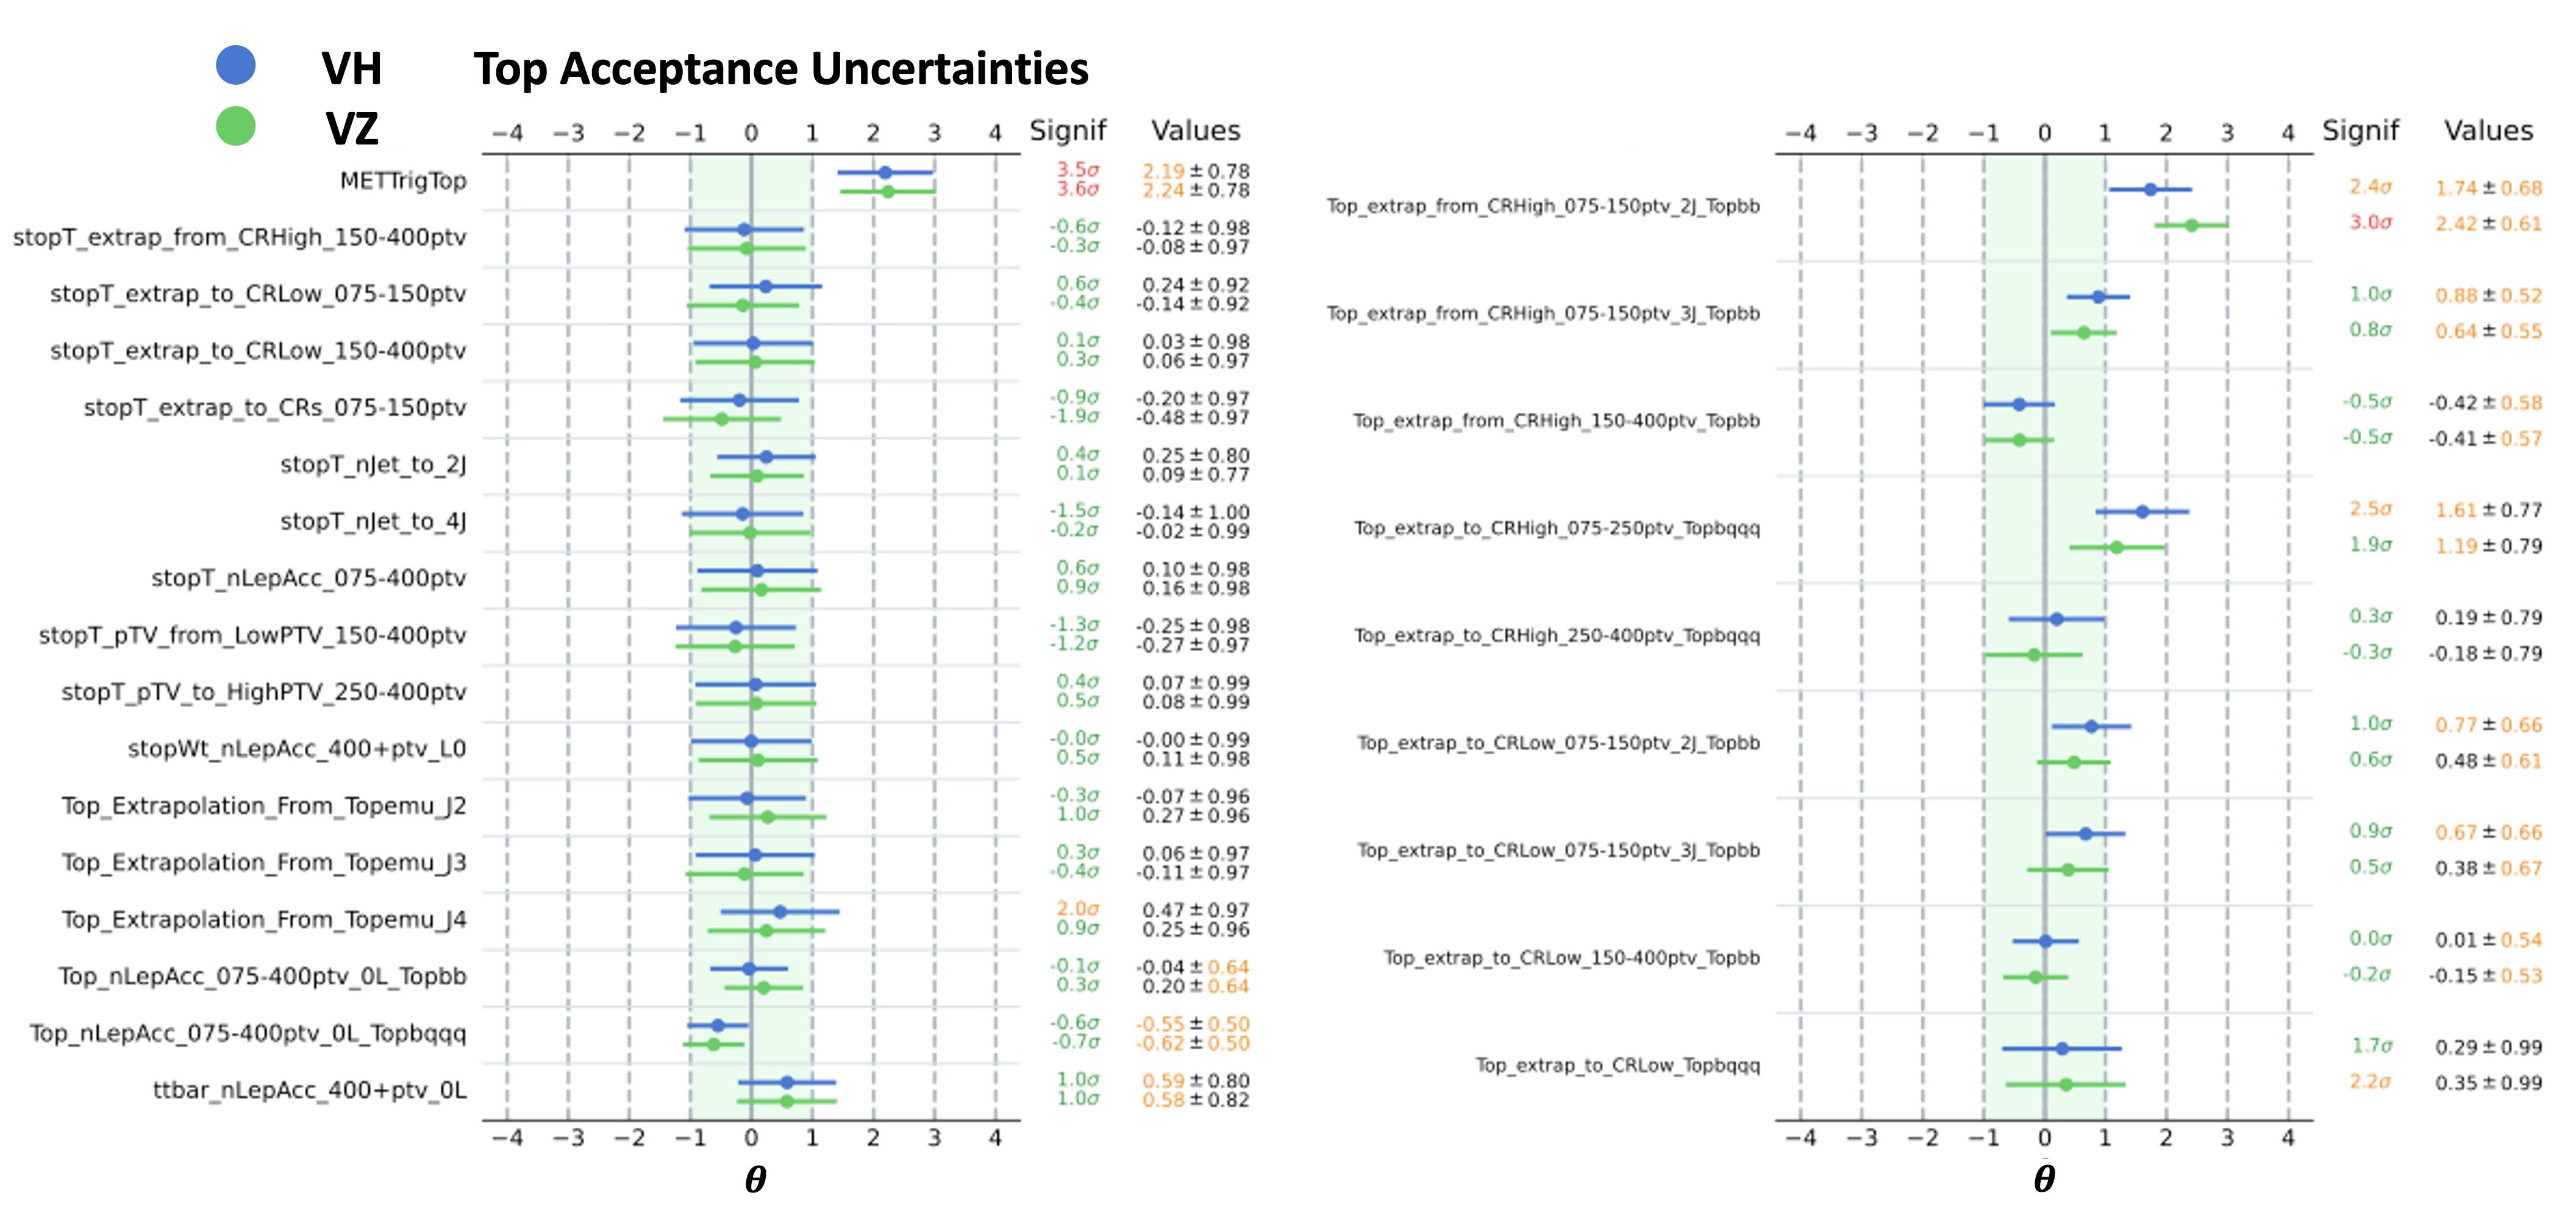
\includegraphics[width=\textwidth]{Images/VH/Fit/fromSlides/FN/top1.png}\\
    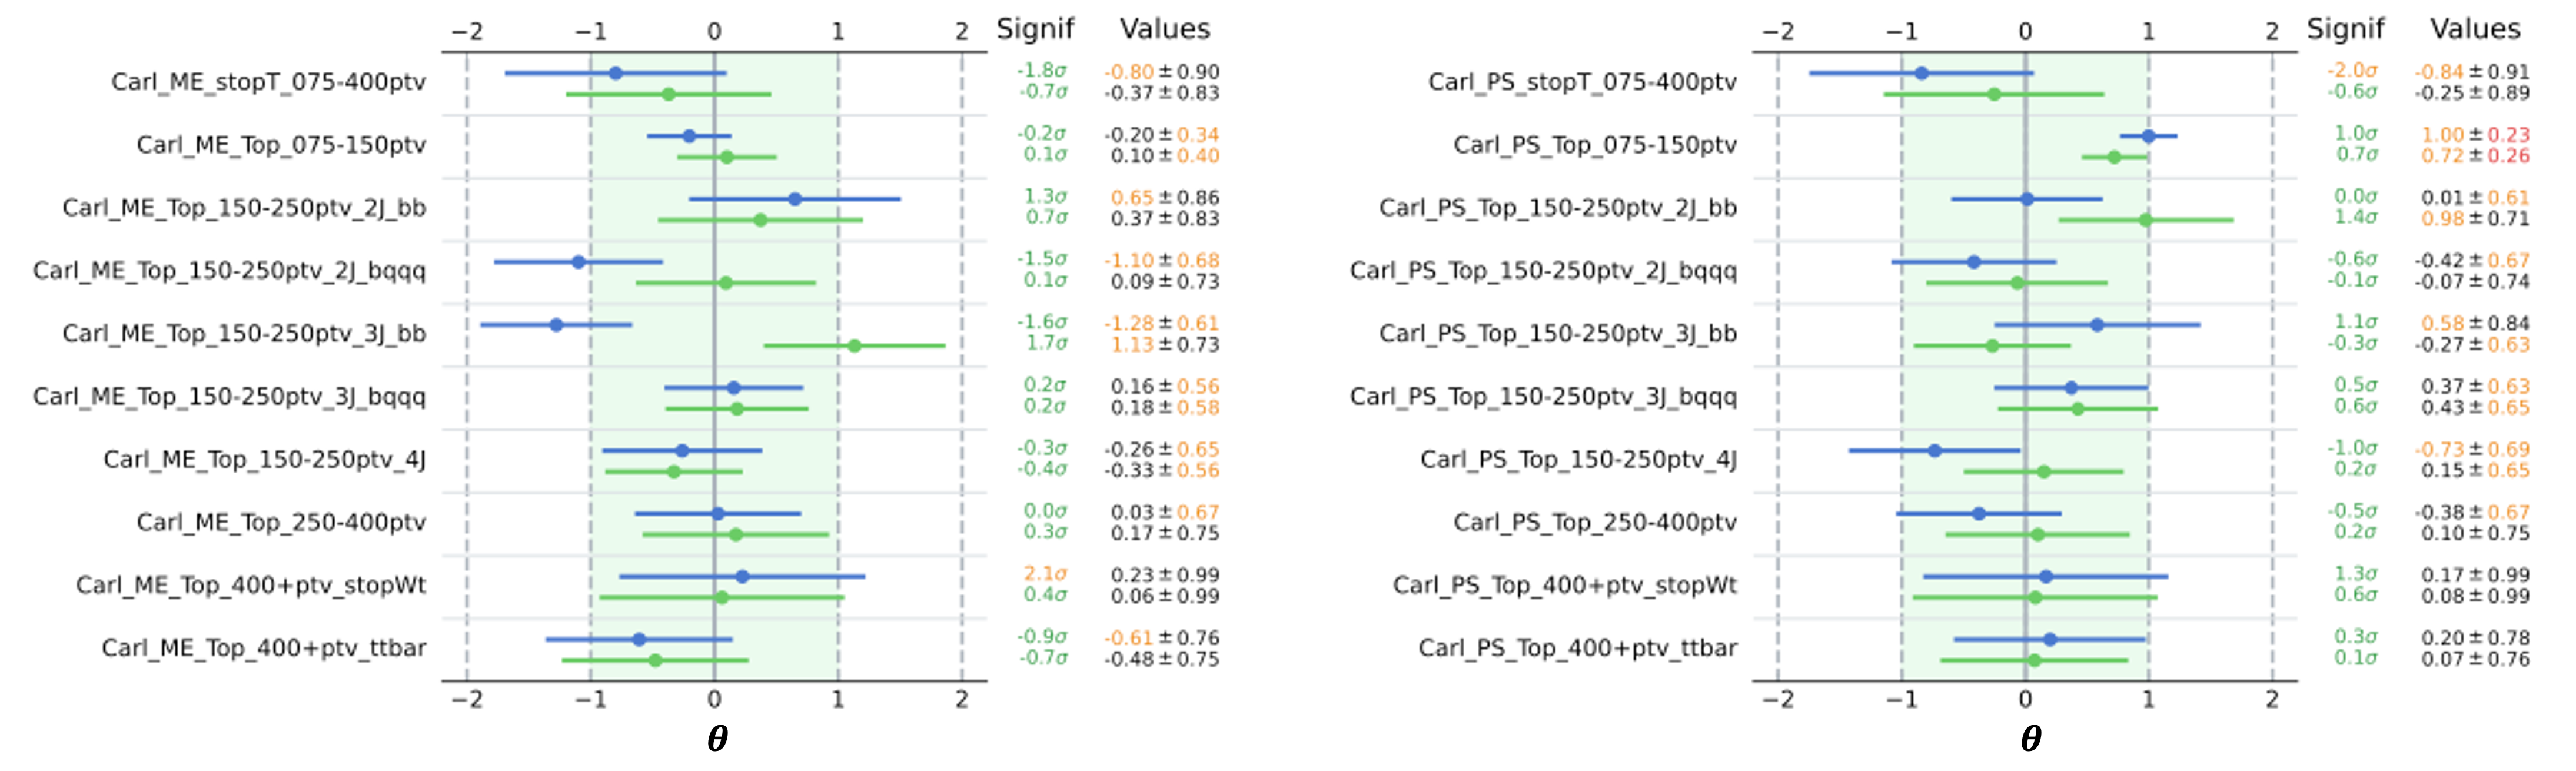
\includegraphics[width=\textwidth]{Images/VH/Fit/fromSlides/FN/top2.png}
    \caption{Some Top nuisance parameters related to acceptance uncertainties (top) and CARL shapes (bottom) in the combined analysis targeting the \vhbc\ in blue, versus the cross-check analysis $VZ(\rightarrow b\bar{b}/c\bar{c})$ in green.}
    \label{apfig:topPull}
\end{figure} 

Other uncertainties presented cover the region extrapolation for the single-top $t$ (left) and combined Top process (right), as well as \nj\ and \ptv\ (for single-top $t$), lepton channel extrapolations, and the extrapolation from the Top $e/\mu$ \gls{cr}. Most of the \glspl{np} are not significantly pulled, with little constraining. This indicates that the fit is not very sensitive nor requires the effect they implement. One exception is the Top$(bb)$ extrapolation from the CRHigh in 75 GeV $<$ \ptv\ $<$ 150 GeV with 2-jet: the \gls{np} is largely pulled, and even more so in the $VZ$ cross-check analysis. This feature can be understood from the large presence of $V+$jets and Top in the 0L and 1L CRHigh, leading to an interplay between the two processes when shifting the focus towards the signal part of $V+$jets. This interplay is visible in the correlation of the boosted \ttb\ and \whf\ in Figure \ref{fig:FNcorr}.

\clearpage
\section{Signal and Background Modelling}\label{appsec-vh-backsigmod}
Additional information on the signal and background modelling is given in this section. Tables \ref{tbl:zjets_acc_full} and \ref{tbl:wjets_acc_full} list the different acceptance uncertainties for the $Z+$jets and $W+$jets respectively in the resolved regime. Tables \ref{tbl:zjets_acc_fullBoos} and \ref{tab:wjets_acc_fullBoos} present $V+$jets uncertainties in the boosted regime. The top-related uncertainties are detailed in Table \ref{tab:top_summary} for the resolved regime and Table \ref{tab:ttbar_summary_boosted} for the boosted regime, while the single-top $t$ is described in Tables \ref{tab:stopt_summary} and \ref{tab:stopt_summary_boosted}. The diboson uncertainties are described in Tables \ref{table:VV_SysBoos_Summary} and \ref{table:VV_Sys_Summary}.

\begin{table}
  \begin{tabular}{l|l|c}
    \hline
    \textbf{Acceptance Ratio Name} & \textbf{Applied} & \textbf{Value} \\
    \hline
    \zhf\ normalistion & \zhf & floating \\
    \zmf\ normalistion & \zmf & floating \\
    \zlf\ normalistion & \zlf & floating \\ 
    \hline
    $Zcc$/$Zbb$ ratio  & $Zcc$ & 12\% \\
    $Zcc$/$Zbb$ ratio  & $Zcc$, \vhb, 2-jet & 8\% \\
    $Zbl$/$Zbc$ ratio  & $Zbl$ & 4\% \\
    $Zbc$/$Zcl$ ratio  & $Zbc$ & 10\% \\
    \hline
    \zhf\ SR/CR ratio & \zhf, 2L, SR, \ptv\ 75-150 & 7\% \\
    \zhf\ SR/CR ratio & \zhf, 2L, SR, \ptv\ >150 & 15\% \\
    \zhf\ SR/CR ratio & \zhf, 0L, SR, TopCR, \ptv\ >150 & 10\% \\
    \zhf\ SR/CR ratio & \zhf, 02L, SR, TopCR, \ptv\ >250, 2-jet & 30\% \\
    \zmf\ SR/CR ratio & \zmf, 2L, SR, \ptv\ 75-150 & 7\% \\
    \zlf\ CR/SR ratio & \zlf, 2L, SR, \ptv\ 75-150 & 7\% \\
    \zmf\ SR/CR ratio & \zmf, 02L, SR, topCR, \ptv\ >150 & 5\% \\
    \zlf\ CR/SR ratio & \zlf, 02L, SR, topCR, \ptv\ >150 & 5\% \\
    \hline
    \zhf\ 0L/2L ratio  & \zhf, 0L, 2-jet & 2\% \\
    \zhf\ 0L/2L ratio  & \zhf, 0L, 3-jet & 4\% \\
    \zhf\ 0L/2L ratio  & \zhf, \vhb\ 0L, 4-jet & 8\% \\
    \zmf\ 0L/2L ratio  & \zhf, 0L, 2-jet & 3\% \\
    \zmf\ 0L/2L ratio  & \zmf, 0L, 3-jet & 8\% \\
    \zlf\ 0L/2L ratio  & \zlf, 0L, 2-jet & 4\% \\
    \zlf\ 0L/2L ratio  & \zlf, 0L, 3-jet & 10\% \\
    \hline
  \end{tabular}
  \caption{$Z+$jets acceptance uncertainties in the resolved regime.}
  \label{tbl:zjets_acc_full}
\end{table}
    

\begin{table}
  \begin{tabular}{l|l|c}
    \hline
    \textbf{Acceptance Ratio Name} & \textbf{Applied} & \textbf{Value} \\
    \zhf\ normalistion & \zhf & floating \\
    \zmf\ normalistion & \zhf & 35\% \\
    \zlf\ normalistion & \zhf & 35\% \\ 
    \hline
    $Zcc/Zbb$ ratio  & $Zcc$ in 02L & 6\% \\
    $Zbl/Zbc$ ratio  & $Zbl$ in 02L & 6\% \\
    $Zcl/Zbc$ ratio  & $Zcl$ in 02L & 6\% \\ 
    \hline
    \zhf\ TopCR/SR ratio  & \zhf, 0L, TopCR & 15\% \\
    \zmf\ TopCR/SR ratio  & \zmf, 0L, TopCR & 25\% \\
    \hline
    0L / 2L ratio & \zhf\ \& \zmf, 0L & 3\% \\
    \hline
    \ptv\ 600 / 400-600  extrap. & \zhf\ \& \zmf, 0L \& 2L & 15\% \\
    \hline \hline
  \end{tabular}
  \caption{$Z+$jets acceptance uncertainties in the boosted regime.}
  \label{tbl:zjets_acc_fullBoos}
\end{table}
    
\begin{table}
  \scriptsize
  \centering
  \resizebox{0.9\textwidth}{!}{
  \begin{tabular}{l|l|c}
    \hline \hline
    \textbf{Acceptance Ratio Name} & \textbf{Applied} & \textbf{Value} \\
    \hline 
    \whf\ normalistion & \whf & floating \\
    \wmf\ normalistion & \wmf & floating \\
    \wlf\ normalistion & \wlf & floating \\ 
    \wlf\ normalistion & \wlf 1L \ptv\ 150-250 & 25\% \\  % TODO from slides
    \hline
    $Wcc/Wbb$ ratio  & $Wcc$, 1L \ptv\ 75-150 & 20\% \\
    $Wcc/Wbb$ ratio  & $Wcc$, 1L \ptv\ >150, 2-jet & 4\% \\
    $Wcc/Wbb$ ratio  & $Wcc$, 1L \ptv\ >150, 3-jet & 15\% \\
    $Wcc/Wbb$ ratio  & $Wcc$, \vhb, 0L, 2-jet & 4\% \\
    $Wcc/Wbb$ ratio  & $Wcc$, \vhb, 0L, 3-jet & 10\% \\
    $Wcc/Wbb$ ratio  & $Wcc$, \vhb, 0L, 4-jet & 10\% \\
    $Wcc/Wbb$ ratio  & $Wcc$, \vhc, 0L & 25\% \\
    $Wbc/Wcl$ ratio  & $Wbc$, \ptv\ 75-150 & 24\% \\
    $Wbc/Wcl$ ratio  & $Wbc$, \ptv\ 150-250, 2-jet & 24\% \\
    $Wbc/Wcl$ ratio  & $Wbc$, \ptv\ 150-250, 3-jet & 14\% \\
    $Wbc/Wcl$ ratio  & $Wbc$, \ptv\ $>$250 & 14\% \\
    $Wbl/Wcl$ ratio  & $Wbl$, \ptv\ 75-150 & 29\% \\
    $Wbc/Wcl$ ratio  & $Wbc$, \ptv\ 150-250, 2-jet & 29\% \\
    $Wbc/Wcl$ ratio  & $Wbc$, \ptv\ 150-250, 3-jet & 22\% \\
    $Wbc/Wcl$ ratio  & $Wbc$, \ptv\ $>$250, 2-jet & 19\% \\
    $Wbc/Wcl$ ratio  & $Wbc$, \ptv\ $>$250, 3-jet & 12\% \\
    $Wbc/Wcl$ ratio  & $Wbc$, 0L, 4-jet & 8\% \\
    $Wq\tau / Wcl$ ratio & $Wc \tau $, $Wb\tau $ & 20\% \\
    $Wl\tau / Wcl$ ratio & $Wl \tau $, $W\tau\tau $ & 9\% \\
    \hline
    \whf\ CRHigh / SR+CRLow ratio & \whf, 1L, CRHigh, \ptv\ 75-150, 2-jet & 3\% \\
    \whf\ CRHigh / SR+CRLow ratio & \whf, 1L, CRHigh, \ptv\ 75-150, 3-jet & 7\% \\
    \whf\ CRHigh / SR+CRLow ratio & \whf, 1L, CRHigh, \ptv\ 150-250, 2-jet & 30\% \\
    \whf\ CRHigh / SR+CRLow ratio & \whf, 1L, CRHigh, \ptv\ 150-250, 3-jet & 10\% \\
    \whf\ CRHigh / SR+CRLow ratio & \whf, 1L, CRHigh, \ptv\ $>$250, 2-jet & 50\% \\
    \whf\ CRHigh / SR+CRLow ratio & \whf, 1L, CRHigh, \ptv\ $>$250, 3-jet & 20\% \\
    \whf\ CRHigh / SR+CRLow ratio & \whf, 0L, CRHigh, 2-jet & 30\% \\
    \whf\ CRHigh / SR+CRLow ratio & \whf, 0L, CRHigh, 3-jet & 20\% \\
    \whf\ CRHigh / SR+CRLow ratio & \whf, 0L, CRHigh, \ptv\ 150-250, 4-jet & 10\% \\
    \whf\ CRHigh / SR+CRLow ratio & \whf, 0L, CRHigh, \ptv\ $>$250, 4-jet & 15\% \\
    \whf\ SR / CRLow ratio  & \whf, 1L, SR, topCR, \ptv\ 75-150, 2-jet & 33\% \\
    \whf\ SR / CRLow ratio  & \whf, 1L, SR, topCR, \ptv\ 75-150, 3-jet & 3\% \\
    \whf\ SR / CRLow ratio  & \whf, 1L, SR, topCR, \ptv\ 150-250, 2-jet & 65\% \\
    \whf\ SR / CRLow ratio  & \whf, 1L, SR, topCR, \ptv\ 150-250, 3-jet & 7\% \\
    \whf\ SR / CRLow ratio  & \whf, 1L, SR, topCR, \ptv\ $>$250, 2-jet & 20\% \\
    \whf\ SR / CRLow ratio  & \whf, 1L, SR, topCR, \ptv\ $>$250, 3-jet & 13\% \\
    \wmf\ CRHigh / SR ratio & \wmf, 1L, CRHigh, CRLow, \ptv\ 75-150, 2-jet & 2\% \\
    \wmf\ CRHigh / SR ratio & \wmf, 1L, CRHigh, CRLow, \ptv\ 75-150, 3-jet & 5\% \\
    \wmf\ SR / CRHigh ratio & \wmf, 01L, SR, topCR, CRLow \ptv\ 150-250 & 7\% \\
    \wmf\ SR / CRHigh ratio & \wmf, 01L, SR, topCR, CRLow \ptv\ $>$250 & 16\% \\
    \wlf\ CRHigh / SR ratio & \wlf, 1L, CRHigh, \ptv\ 75-150, 2-jet & 5\% \\
    \wlf\ CRHigh / SR ratio & \wlf, 1L, CRHigh, \ptv\ 75-150, 3-jet & 10\% \\
    \wlf\ CRHigh / SR ratio & \wlf, 01L, CRHigh, \ptv\ 150-250, 2-jet & 5\% \\
    \wlf\ CRHigh / SR ratio & \wlf, 01L, CRHigh, \ptv\ 150-250, 3-jet & 10\% \\
    \wlf\ CRHigh / SR ratio & \wlf, 01L, CRHigh, \ptv\ $>$250, 2-jet, 3-jet & 17\% \\
    \hline
    \whf\ 4-jet / 3-jet ratio & \whf, 0L, \ptv\ 150-250, 4-jet & 12\% \\
    \whf\ 4-jet / 3-jet ratio & \whf, 0L, \ptv\ $>$250, 4-jet & 20\% \\
    \hline
    \whf\ 0L / 1L ratio & \whf, 0L, \ptv\ 150-250, 2-jet & 30\% \\
    \whf\ 0L / 1L ratio & \whf, 0L, \ptv\ 150-250, 3(+)-jet & 20\% \\
    \whf\ 0L / 1L ratio & \whf, 0L, \ptv\ $>$250, 2-jet & 20\% \\
    \whf\ 0L / 1L ratio & \whf, 0L, \ptv\ $>$250, 3(+)-jet & 13\% \\
    \wmf\ 0L / 1L ratio & \wmf, 0L, \ptv\ 150-250, 2-jet & 3\% \\
    \wmf\ 0L / 1L ratio & \wmf, 0L, \ptv\ 150-250, 3-jet & 8\% \\
    \wmf\ 0L / 1L ratio & \wmf, 0L, \ptv\ $>$250 & 10\% \\
    \wlf\ 0L / 1L ratio & \wlf, 0L & 4\% \\
    \hline \hline
  \end{tabular}
  }
  \caption{The $W+$jets acceptance uncertainties in the resolved regime.}
  \label{tbl:wjets_acc_full}
\end{table}
    

\begin{table}
  %\scriptsize
  \centering
  \begin{tabular}{l|l|c}
    \hline \hline
    \textbf{Acceptance Ratio Name} & \textbf{Applied} & \textbf{Value} \\ \hline
    \whf\ normalistion & \whf & floating \\
    \wmf\ normalistion & \whf & 36\% \\
    \wlf\ normalistion & \whf & 38\% \\ 
    \hline
    $Wcc/Wbb$ ratio & $Wcc$ & 11\% \\
    $Wcl/Wbc$ ratio & $Wcl$ & 15\% \\ 
    $Wbl/Wbc$ ratio & $Wbl$ & 9\% \\
    \hline
    \whf\ TopCR / SR ratio & \whf, 0L \& 1L, TopCR & 27\% \\
    \wmf\ TopCR / SR ratio & \wmf, 0L \& 1L, TopCR & 20\% \\
    \wlf\ TopCR / SR ratio & \wlf, 0L \& 1L, TopCR & 16\% \\
    \hline
    0L / 1L ratio  & All, 0L & 20\% \\
    \hline
    \ptv\ $>$600 / 400-600 GeV ratio & \wmf \& \wlf, 0L \& 1L & 3\% \\
    \hline \hline
  \end{tabular}
  \caption{The $W+$jets acceptance uncertainties in the boosted regime.}
  \label{tab:wjets_acc_fullBoos}
\end{table}
      


\begin{table}[!htpb] 
    \begin{center}
    \selectfont 
    \centering \resizebox{\columnwidth}{!}{         
    \begin{tabular}{ l | l | c  } 
    \hline \hline
    \textbf{Acceptance Ratio Name} & \textbf{Applied} & \textbf{Value} \\
    \hline
    Top$(bb)$ normalisation     & 0L \& 1L, decorr in \nj \& \ptv & floating \\
    Top$(bb)$ normalisation     & \vhc\ $e\mu$ CR \ 2L & floating \\ 
    Top$(bq/qq)$ normalisation  & 0L \& 1L, decorr in \nj\ \& \ptv & floating \\ 
    \hline
    Top $bl$ / $bc$ Ratio     & 01L, Top$(bl)$ & 5 \%  \\
    Top $qq$ / $bc+bl$ ratio  & 01L, Top$(qq)$ & 10 \%  \\
    \hline
    Top$(bb)$ CRLow+SR / CRHigh ratio    & 01L, CRLow, SR, TopCR, Top$(bb)$ & 2 \% (75-250 GeV) 8 \% (250-400 GeV) \\
    Top$(bb)$ CRLow / SR ratio           & \vhb\ 1L, CRLow, Top$(bb)$ & 2.5 \% (75-150 GeV) 9 \% (150-400 GeV) \\
    Top$(bq/qq)$ CRHigh / CRLow+SR ratio & 01L, CRHigh, Top$(bq/qq)$ & 4 \% (75-250 GeV) 10 \% (250-400 GeV) \\
    Top$(bq/qq)$ CRLow / SR ratio        & \vhb\ 1L, CRLow, Top$(bq/qq)$ & 2.5 \% (75-250 GeV) 4 \% (250-400 GeV) \\
    Top SR / Top $e\mu$ CR               & \vhb\ 2L & 0.8\% \\
    \hline
    $Wt$ / \ttb\ ratio & 0L, $Wt(bb)$ & 22 \% (150-250 GeV) 48 \% (250-400 GeV) \\
    $Wt$ / \ttb\ ratio & 1L, $Wt(bb)$ & 15 \% (75-150 GeV) 13 \% (150-400 GeV) \\
    $Wt$ / \ttb\ ratio & 01L, $Wt(bq/qq)$ & 12 \% (75-250 GeV) 18 \% (250-400 GeV) \\
    \hline
    Top 0L / 1L ratio & 0L & 2 \% (150-250 GeV) 8 \% (250-400 GeV) \\ 
    \hline
    \gls{carl} ME Top shape & 01L & $-$ \\
    \gls{carl} PS Top shape & 01L & $-$ \\
    $Wt$ DS/DR shape + normalisation & $Wt$, 01L & $-$ \\
    \gls{isr} Top shape & 01L & $-$ \\
    \gls{fsr} Top shape & 01L & $-$ \\
    \hline
    \hline
    \end{tabular}} 
    \caption{Resolved regime Top (\ttb\ + $Wt$) uncertainties.}
    \label{tab:top_summary}
    \end{center}
\end{table}

\begin{table}[!htpb] 
    \begin{center}
    \centering \resizebox{\columnwidth}{!}{         
    \begin{tabular}{ l | l | c  } 
    \hline \hline
    \textbf{Acceptance Ratio Name} & \textbf{Applied} & \textbf{Value} \\
    \hline 
    \ttb\ normalisation & \ttb, 01L, decorr. in \ptv & floating \\ %check name
    \ttb\ normalisation & \ttb, 2L & 20\% \\ %check name
    $Wt$ normalisation & \ttb, 012L & 25\% \\ %check name
    \hline
    \ttb\ SR / TopCR ratio & \ttb, 01L, SR &  10\%  \\
    \hline
    \ttb\ 0L / 1L ratio & \ttb, 0L & 6\% (400-600 GeV) 20\% (600+ GeV)  \\
    $Wt$ 0L / 1L ratio & \ttb, 0L & 20\% (400-600 GeV) 40\% (600+ GeV)  \\
    %\hline
    %$Wt$ / \ttb ratio & $Wt$, 01L & 22\% (400-600 GeV)  36\% (600+ GeV)  \\
    $Wt$ \ptv\ $>$600 / 400-600 GeV ratio & $Wt$, 01L 400-600 GeV & 20\% \\
    \hline
    \gls{carl} ME \ttb\ shape & \ttb, 01L & $-$ \\
    \gls{carl} PS \ttb\ shape & \ttb, 01L & $-$ \\
    \gls{carl} ME  $wt$ shape & \ttb, 01L & $-$ \\
    \gls{carl} PS  $wt$ shape & \ttb, 01L & $-$ \\
    \gls{isr} \ttb\ shape & \ttb, 01L & $-$  \\
    \gls{fsr} \ttb\ shape & \ttb, 01L & $-$  \\
    \gls{isr} $wt$ shape & \ttb, 01L & $-$  \\
    \gls{fsr} $wt$ shape & \ttb, 01L & $-$  \\
    \hline \hline
    \end{tabular} 
    } 
    \caption{Boosted regime \ttb\ and $Wt$ uncertainties.} 
    \label{tab:ttbar_summary_boosted}
    \end{center}
\end{table} 


\begin{table}[!htpb] 
    \begin{center}
    \selectfont 
    \centering \resizebox{\columnwidth}{!}{         
    \begin{tabular}{ l | l | c  } 
    \hline \hline
    \textbf{Acceptance Ratio Name} & \textbf{Applied} & \textbf{Value} \\
    \hline
    stop-$t$ normalisation& 01L, all regions & 17 \% \\ 
    \hline
    stop-$t$ CRLow+CRHigh / SR  ratio  & 1L, 75-150 GeV, CRHigh and CRLow  & 3 \%  \\
    stop-$t$ CRLow / CRHigh ratio      & 1L, 75-150 GeV, CRLow             & 6 \%  \\
    stop-$t$ CRLow+SR / CRHigh ratio   & 01L, SR, TopCR, CRLow, decorr. 150-250 and 250-400 GeV & 6 \%  \\
    stop-$t$ CRLow / SRratio           & 01L, CRLow, decorr. 150-250 and 250-400 GeV & 17 \% \\
    \hline
    stop-$t$ 2-jet / 3-jet ratio   & 01L, 2-jet region & 15 \% \\
    stop-$t$ 4-jet / 2+3-jet ratio & 0L, 4-jet region & 15 \% \\
    \hline
    stop-$t$ \ptv 150-400 / 75-150 ratio  & 01L, decorr. 150-250 and 250-400 GeV & 7 \%  \\
    stop-$t$ \ptv 250-400 / 150-250 ratio & 01L, 250-400 GeV & 15 \%  \\
    \hline
    Sysstopt\_nLepAcc & 0L / 1L & 0L & 6 \% \\
    \hline
    \gls{carl} ME stop-$t$ shape & 01L & $-$ \\
    \gls{carl} PS stop-$t$ shape & 01L & $-$ \\
    \gls{isr} stop-$t$ shape & 01L & $-$ \\
    \gls{fsr} stop-$t$ shape & 01L & $-$ \\
    \hline
    \hline
    \end{tabular}} 
    \caption{Resolved regime single-top $t$ (stop-$t$) uncertainties. The single-top $s$ is applied a global 4.6\% normalisation.}
    \label{tab:stopt_summary}
    \end{center}
\end{table}

\begin{table}[!htpb] 
    \begin{center}     
    \begin{tabular}{ l | l | c  } 
    \hline \hline
    \textbf{Acceptance Ratio Name} & \textbf{Applied} & \textbf{Value} \\
    \hline 
    stop-$t$ normalisation & 01L, all regions & 10 \% \\ 
    \hline
    \gls{isr} stop-$t$ shape & 01L & $-$ \\
    \gls{fsr} stop-$t$ shape & 01L & $-$ \\
    \hline
    \hline
    \end{tabular}
    \caption{Boosted regime single-top $t$ (stop-$t$) uncertainties.}
    \label{tab:stopt_summary_boosted}
    \end{center}
\end{table}


\begin{table}[h!]
    %\selectfont 
    \hspace{-1cm}
    \resizebox{1.1\textwidth}{!}
    {
     \begin{tabular}{ c | c | c | c | c } 
     \hline \hline
     NP Name & Description & Production mode & Decay component & Applied regions\\ [0.5ex] 
     \hline 
     ZZNorm & Total acceptance var. & $qqZZ$ & All & 17\%   \\ 
     WZNorm & Total acceptance var. & $qqWZ$ & All & 19\%   \\ 
     WWNorm & Total acceptance var. & $qqWW$ & All & 16\%   \\ 
     $ggVV$Norm & Total acceptance var. & $ggVV$ & All & 30\% \\ 
     \hline
     ZZ\_nLepAcc\_L0 & 2L to 0L ratio & $qqZZ$ & $VZbb$, $VZcc$ & 2\%-3.5\%-23\% in 2-, 3-, 4-jet 0L  \\ 
     WZ\_nLepAcc\_L0 & 1L to 0L ratio & $qqWZ$ & $VZbb$, $VZcc$ & 4\%-10\% in 2-, 3-jet 0L  \\
     WW\_nLepAcc\_L0 & 1L to 0L ratio & $qqWW$ & $VW$bkg & 3\% in 0L \\ 
     WZlephadbkg\_nLepAcc\_L0 & 1L to 0L ratio & $qqWZ$ & $VZ$bkg & 7\% in 0L    \\
     WZhadlep\_nLepAcc\_L0 & 2L to 0L ratio & $qqWZ$ & $VW$bkg & 11\% in 0L       \\ 
     ZZbkg\_nLepAcc\_L0 & 2L to 0L ratio & $qqZZ$ & $VZ$bkg & 12\% in 0L          \\
     ZZ\_extrap\_to\_CRHigh & SR to CRHigh ratio & $qqZZ$ & $VZbb$, $VZcc$ & 20\% in 0L \& 15\%-20\% in 2L     \\ 
     WZ\_extrap\_to\_CRHigh & SR to CRHigh ratio & $qqWZ$ & $VZbb$, $VZcc$ & 12\% in 0L \& 13\%-20\% in 1L     \\ 
     WZ\_extrap\_to\_CRLow & SR+CRHigh to CRLow ratio & $qqWZ$ & $VZbb$, $VZcc$ & 50\%-18\% in 1L  \\ 
     WW\_extrap\_to\_CRHigh & SR to CRHigh ratio & $qqWW$ & $VW$bkg & 10\% in 0L \& 16\% in 1L        \\ 
     WZhadlep\_extrap\_to\_CRHigh & SR to CRHigh ratio & $qqWZ$ & $VW$bkg & 14\%-12\%-17\% in 0L-1L-2L   \\ 
     WZlephadbkg\_extrap\_to\_CRHigh & SR to CRHigh ratio & $qqZZ$ & $VZ$bkg & 10\% in 0L \&  11 \% in 1L \\ 
     ZZbkg\_extrap\_to\_CRHigh & SR to CRHigh ratio & $qqWZ$ & $VZbb$, $VZ$bkg & 10\% in 0L \& 28\% in 2L \\ 
     ZZ\_nJAcc\_J3 & 2-jet to 3-jet ratio & $qqZZ$ & $VZbb$, $VZcc$ & 10\% in 0L \& 7\%-10\% in 2L \\ 
     WZ\_nJAcc\_J3 & 2-jet to 3-jet ratio & $qqWZ$ & $VZbb$, $VZcc$ & 25\% in 0L \& 20\%-25\% in 1L  \\ 
     ZZ\_nJAcc\_J4 & 3-jet to 4(4+)-jet ratio & $qqZZ$ & $VZbb$, $VZcc$ & 16\% in 0L \& 30\% in 2L \\ 
     WZ\_nJAcc\_J4 & 3-jet to 4-jet ratio & $qqWZ$ & $VZbb$, $VZcc$ & 16\% in 0L \\ 
     WW\_nJAcc\_J3p & 2-jet to 3+-jet ratio & $qqWW$ & $VW$bkg & 12\% in 0L \& 1L \\ 
     WZhadlep\_nJAcc\_J3p & 2-jet to 3+-jet ratio & $qqWZ$ & $VW$bkg & 13\%-10\%-24\% in 0L-1L-2L  \\  
     WZlephadbkg\_nJAcc\_J3p & 2-jet to 3+-jet ratio & $qqWZ$ & $VZ$bkg & 14\% in 0L \& 11\% in 1L \\ 
     ZZbkg\_nJAcc\_J3p & 2-jet to 3+-jet ratio & $qqZZ$ & $VZ$bkg & 10\% in 0L \& 28\% in 2L\\  
     %WW\_nJAcc\_J4 & 3-jet to 4-jet ratio & $qqWW$ & $VW$bkg & 0L 4-jet \\  % TODO no value? Not found in src
     WZ\_nJAcc\_J4 & 3-jet to 4+-jet ratio & $qqWZ$ & $VW$bkg & 16\% in 0L \\ % Note: the 4J values are from reading the WSMaker
     %WZlephadbkg\_nJAcc\_J4 & 3-jet to 4-jet ratio & $qqWZ$ & $VZ$bkg & 0L 4-jet \\   % TODO not found
     ZZbkg\_nJAcc\_J4 & 3-jet to 4+-jet ratio & $qqZZ$ & $VZ$bkg & 16\% 0L \& 30\% 2L \\  
     ZZ\_ptvAcc\_250-400 & \ptv [150,250] to [250,400] ratio & $qqZZ$ & $VZbb$, $VZcc$ & 3\%-9\% in 0L \& 2L \\ 
     ZZ\_ptvAcc\_075-150 & \ptv [150,250] to [75,150] ratio & $qqZZ$ & $VZbb$, $VZcc$ & 6\% in 2L  \\ 
     WZ\_ptvAcc\_250-400 & \ptv [150,250] to [250,400] ratio & $qqWZ$ & $VZbb$, $VZcc$ & 4\%-16\% in 0L \& 4\% 1L \\ 
     WZ\_ptvAcc\_075-150 & \ptv [150,250] to [75,150] ratio & $qqWZ$ & $VZbb$, $VZcc$ & 2\%-5\% in 1L  \\ 
     WW\_ptvAcc\_075-150 & \ptv [150,250] to [75,150] ratio & $qqWW$ & $VW$bkg & 5\% in 1L  \\ 
     WZhadlep\_ptvAcc\_075-150 & \ptv [150,250] to [75,150] ratio & $qqWZ$ & $VW$bkg & 4\% in 1L \& 2L     \\ 
     WZlephadbkg\_ptvAcc\_075-150 & \ptv [150,250] to [75,150] ratio & $qqWZ$ & $VZ$bkg & 3\% in 1L \& 5\% in 2L \\ 
     ZZbkg\_ptvAcc\_075-150 & \ptv [150,250] to [75,150] ratio & $qqZZ$ & $VZ$bkg & 4\% 2L \\ 
     WW\_ptvAcc\_250-400 & \ptv [150,250] to [250,400] ratio & $qqWW$ & $VW$bkg & 9\% in 0L \& 1L  \\ 
     WZhadlep\_ptvAcc\_250-400 & \ptv [150,250] to [250,400] ratio & $qqWZ$ & $VW$bkg & 10\% in all channels  \\ 
     WZlephadbkg\_ptvAcc\_250-400 & \ptv [150,250] to [250,400] ratio & $qqWZ$ & $VZ$bkg & 9\% in all channels \\ 
     ZZbkg\_ptvAcc\_250-400 & \ptv [150,250] to [250,400] ratio & $qqZZ$ & $VZ$bkg & 7\% in 0L \& 2L  \\ 
     \hline
     ZZQCDscale\_d150 &  \ptv [75,150] to [150,400] \gls{qcd} migration & $qqZZ$ & $VZbb$, $VZcc$ & -3.2\% to 7.8\% in 1L \& 2L \\
     WZQCDscale\_d150 &  \ptv [75,150] to [150,400] \gls{qcd} migration & $qqWZ$ & $VZbb$, $VZcc$ & -3.1\% to 5.8\% in 1L \& 2L \\
     ZZQCDscale\_d250 & \ptv [150,250] to [250,400] \gls{qcd} migration & $qqZZ$ & $VZbb$, $VZcc$ & -2.4\% to 8.4\%  \\ 
     WZQCDscale\_d250 & \ptv [150,250] to [250,400] \gls{qcd} migration & $qqWZ$ & $VZbb$, $VZcc$ & -1.6\% to 7.9\%  \\
     ZZQCDscale\_dJ3 & 2-jet to 3,4(4+)-jet \gls{qcd} migration & $qqZZ$ & $VZbb$, $VZcc$ & -35.6\% to 19.9\% \\ 
     WZQCDscale\_dJ3 & 2-jet to 3,4(4+)-jet \gls{qcd} migration & $qqWZ$ & $VZbb$, $VZcc$ & -37.4\% to 16.2\% \\ 
     ZZQCDscale\_dJ4 &   3-jet to 4(4+)-jet \gls{qcd} migration & $qqZZ$ & $VZbb$, $VZcc$ & -30\% to 32\% in 0L \& 2L \\ 
     WZQCDscale\_dJ4 &   3-jet to 4(4+)-jet \gls{qcd} migration & $qqWZ$ & $VZbb$, $VZcc$ & -14.7\% to 23.2\% in 0L  \\ 
     \hline
     Carl\_ZZ\_Sh2211toPwPy8 & \textsc{Powheg} + \textsc{Pythia} 8 \gls{carl} shape var. & $qqZZ$ & All & 0L \& 2L \\ 
     Carl\_ZZ\_Sh2211toSh221 & \textsc{Sherpa} 2.2.1 \gls{carl} shape var. & $qqZZ$ & All & 0L \& 2L \\
     Carl\_WZ\_Sh2211toPwPy8 & \textsc{Powheg} + \textsc{Pythia} 8 \gls{carl} shape var. & $qqZZ$ & All & 0L \& 1L (2L in \vhc\ only) \\
     Carl\_WZ\_Sh2211toSh221 & \textsc{Sherpa} 2.2.1 \gls{carl} shape var. & $qqZZ$ & All & 0L \& 1L (2L in \vhc\ only) \\
     Carl\_WW\_Sh2211toPwPy8 & \textsc{Powheg} + \textsc{Pythia} 8 \gls{carl} shape var. & $qqZZ$ & All & 0L \& 1L in \vhc\ \\
     Carl\_WW\_Sh2211toSh221 & \textsc{Sherpa} 2.2.1 \gls{carl} shape var. & $qqZZ$ & All & 0L \& 1L in \vhc\ \\
     \gls{qcd} scale shape & \textsc{Sherpa} 2.2.11 \gls{qcd} scale largest shape var. & qqVV & All & Inclusive region in 1L \& 2L \\
     \gls{ew} shape & \textsc{Sherpa} 2.2.11 \gls{ew} Correction largest shape var. & qqVV & All & Inclusive region in 1L \& 2L \\
     \hline \hline
     \end{tabular}
    }
    \caption{Diboson uncertainties in the resolved regime.} 
     \label{table:VV_Sys_Summary}
\end{table}
    

\begin{table}[h!]
    %\selectfont 
    \hspace{-1cm}
    \resizebox{1.1\textwidth}{!}
    {
     \begin{tabular}{ c | c | c | c | c } 
     \hline \hline
     NP Name & Description & Production mode & Decay component & Applied regions\\ [0.5ex] 
     \hline 
     ZZNorm\_boosted & Total acceptance var. & $qqZZ$ & All & 17\% \\ 
     WZNorm\_boosted & Total acceptance var. & $qqWZ$ & All & 27\% \\ 
     WWNorm & Total acceptance var. & $qqWW$ & All & 16\%   \\ 
     $ggVV$Norm & Total acceptance var. & $ggVV$ & All & 30\% \\ 
     \hline
     ZZ\_nLepAcc\_boosted\_L0 & 2L to 0L ratio & $qqZZ$ & $VZbb$ & 7\% \\ 
     WZ\_nLepAcc\_boosted\_L0 & 1L to 0L ratio & $qqWZ$ & $VZbb$ & 7\% \\
     (ZZ\_nJAcc\_boosted)$^*$ & HP to LP ratio & $qqZZ$ & $VZbb$, $VZcc$ & 10\% 0L LP \\ 
     (WZ\_nJAcc\_boosted)$^*$ & HP to LP ratio & $qqWZ$ & $VZbb$, $VZcc$ & 15\% 0L \& 1L in LP \\ 
     ZZ\_ptvAcc\_boosted\_Min400 & \ptv [400,600] to [600,] ratio & $qqZZ$ & $VZbb$, $VZcc$ & 8\% in 0L \& 2L \\ 
     WZ\_ptvAcc\_boosted\_Min400 & \ptv [400,600] to [600,] ratio & $qqWZ$ & $VZbb$, $VZcc$ & 40\% in 0L \& 7\% in 1L \\ 
     \hline
     ZZQCDscale\_d600 & \ptv [400,600] to [600,] \gls{qcd} migration & $qqZZ$ & $VZbb$, $VZcc$ & -1.6\% to 7.6\% in 0L \& 2L \\ 
     WZQCDscale\_d600 & \ptv [400,600] to [600,] \gls{qcd} migration & $qqWZ$ & $VZbb$, $VZcc$ & -2.2\% to 10.6\% in 0L \& 1L \\ 
     (ZZQCDscale\_dJ1)$^*$ & HP to LP \gls{qcd} migration & $qqZZ$ & $VZbb$, $VZcc$ & -17.8\% to 16.3\% 0L  \\ 
     (WZQCDscale\_dJ1)$^*$ & HP to LP \gls{qcd} migration & $qqWZ$ & $VZbb$, $VZcc$ & -42.2\% to 19.2\% 0L \& 1L \\ 
     \hline
     Carl\_ZZ\_Sh2211toPwPy8 & \textsc{Powheg} + \textsc{Pythia} 8 \gls{carl} shape var. & $qqZZ$ & All & 0L \& 2L \\ 
     Carl\_ZZ\_Sh2211toSh221 & \textsc{Sherpa} 2.2.1 \gls{carl} shape var. & $qqZZ$ & All & 0L \& 2L \\
     Carl\_WZ\_Sh2211toPwPy8 & \textsc{Powheg} + \textsc{Pythia} 8 \gls{carl} shape var. & $qqZZ$ & All & 0L \& 1L \\
     Carl\_WZ\_Sh2211toSh221 & \textsc{Sherpa} 2.2.1 \gls{carl} shape var. & $qqZZ$ & All & 0L \& 1L \\
     \gls{qcd} scale shape & \textsc{Sherpa} 2.2.11 \gls{qcd} scale largest shape var. & qqVV & All & Inclusive region in 1L \& 2L \\
     \gls{ew} shape & \textsc{Sherpa} 2.2.11 \gls{ew} Correction largest shape var. & qqVV & All & Inclusive region in 1L \& 2L \\
     \hline \hline
     \end{tabular}
    }
    \caption{Diboson uncertainties in the boosted regime.} 
     \label{table:VV_SysBoos_Summary}
\end{table}

\clearpage
\section{Analysis Postfit Regions}\label{appsec-vh-analRegPosfit}
\addtocontents{toc}{\protect\setcounter{tocdepth}{1}}
\subsection{Resolved Postfit Regions}\label{appsec-vh-analRegResPosfit}
All regions in the resolved regime of the combined \vhbc\ analysis after the conditional fit to data of Section \ref{sec-fitFramework} are presented here, organised by increasing number of charged lepton channels (0L, 1L, 2L). The distributions indicate the pre-fit expectations of the sum of processes in dashed blue lines and highlight multiples (for visibility) of either the \vhb\ or \vhc\ signal distributions in red lines. The distribution variables presented, \gls{bdt}, \ptv, etc., correspond to the one used in the fit. Figures \ref{fig:plots_VHbb_OL_SR}, \ref{fig:plots_VHbb_1L_SR}, and \ref{fig:plots_VHbb_2L_SR} are the $BB$-tagged signal regions. The 2 $c$-tagged \glspl{sr} are displayed in Figures \ref{fig:plots_VHcc_OL_SR_2c}, \ref{fig:plots_VHcc_1L_SR_2c}, and \ref{fig:plots_VHcc_2L_SR_2c}. The 1 $c$-tagged \glspl{sr} are displayed in Figures \ref{fig:plots_VHcc_OL_SR_1c}, \ref{fig:plots_VHcc_1L_SR_1c}, and \ref{fig:plots_VHcc_2L_SR_1c}. \\

The different control regions presented can be grouped as:
\begin{itemize}
  \item The $BB$-tagged \highdr\ \glspl{cr} in Figures \ref{fig:plots_VHbb_OL_CRH}, \ref{fig:plots_VHbb_1L_CRH}, and \ref{fig:plots_VHbb_2L_CRH}.
  \item The $c$-tagged ($TN$, $TL$, and $TT$) \highdr\ \glspl{cr} in Figures \ref{fig:plots_VHcc_OL_CRH_2c_2J}, \ref{fig:plots_VHcc_OL_CRH_2c_3J}, \ref{fig:plots_VHcc_1L_CRH_2J}, \ref{fig:plots_VHcc_1L_CRH_3J}, \ref{fig:plots_VHcc_2L_CRH_2J}, and \ref{fig:plots_VHcc_2L_CRH_3J}.
  \item The 1L $BB$-tagged \lowdr\ \glspl{cr} in Figure \ref{fig:plots_VHbb_1L_CRL}.
  \item The 1L and 2L $V+l$ \glspl{cr} ($LN$-tagged) in Figures \ref{fig:plots_VHcc_1L_LN} and \ref{fig:plots_VHcc_2L_LN}.
  \item The 0L and 1L top \glspl{cr} $BT$-tagged in Figures \ref{fig:plots_VHcc_OL_TopCR_2c} and \ref{fig:plots_VHcc_1L_TopCR}.
  \item The 2L top $e\mu$ \glspl{cr} with $\geq$ 1 $T$-tag in Figure \ref{fig:plots_VHcc_2L_topCRemu}.
\end{itemize}
  
\subsection{Boosted Postfit Regions}\label{appsec-vh-analRegBooPosfit}
This section presents the boosted regime regions after the conditional fit, with Figure \ref{fig:plots_VHbbBoost_OL} presenting the 0L regions, Figure \ref{fig:plots_VHbbBoost_1L} the 1L regions, and Figure \ref{fig:plots_VHbbBoost_2L_SR} the 2L regions. The distribution variables presented correspond to the ones used in the fit.

\clearpage

\begin{figure}[h!]
    \centering
    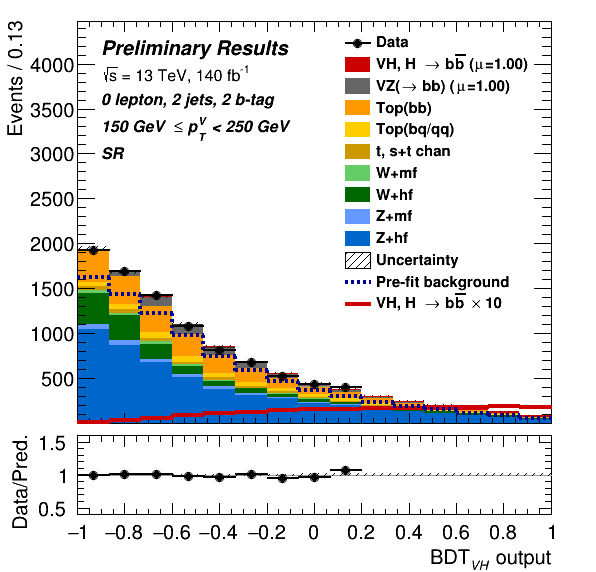
\includegraphics[width=0.32\textwidth]{Images/VH/postfit_VHbb/ZeroLep/Region_distmva_BMax250_BMin150_DSR_J2_TTypebb_T2_L0_Y6051_GlobalFit_conditionnal_mu1.pdf}
    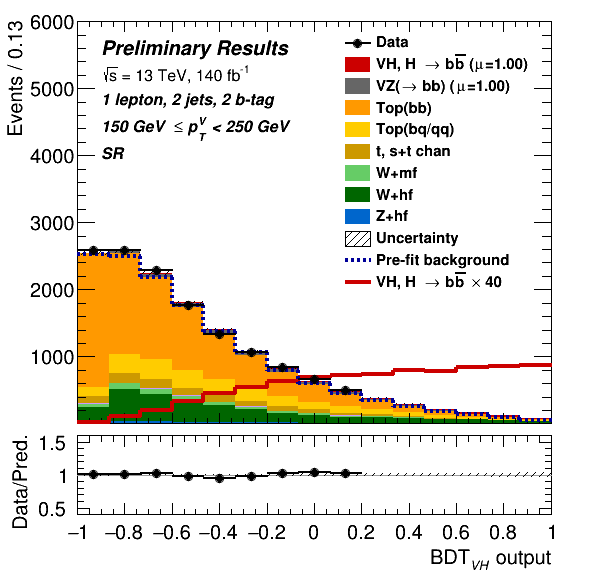
\includegraphics[width=0.32\textwidth]{ Images/VH/postfit_VHbb/OneLep/Region_distmva_BMax250_BMin150_DSR_J2_TTypebb_T2_L1_Y6051_GlobalFit_conditionnal_mu1.pdf}
    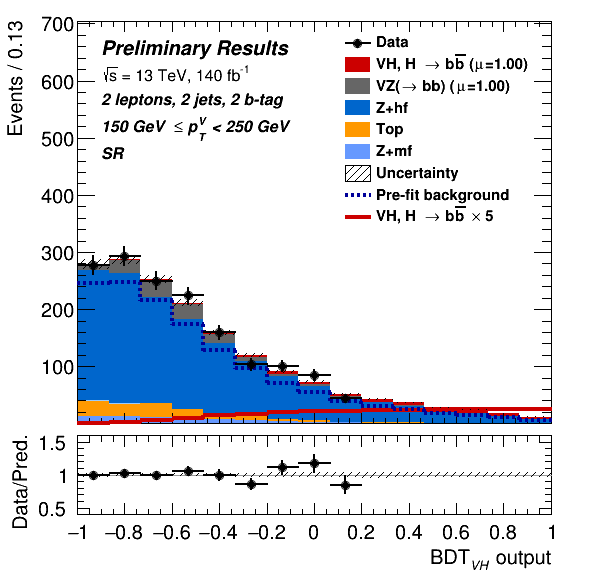
\includegraphics[width=0.32\textwidth]{ Images/VH/postfit_VHbb/TwoLep/Region_distmva_BMax250_BMin150_DSR_J2_TTypebb_T2_L2_Y6051_GlobalFit_conditionnal_mu1.pdf}
    \caption{The \vhb\ posfit conditional distribution in the 150 < \ptv\ < 250 GeV 2-jet signal region in the 0L (left), 1L (centre), and 2L (right).}
    \label{fig:plotsVHBSR_150pt_2J}
  \end{figure} 
  
  \begin{figure}[h!]
    \centering
    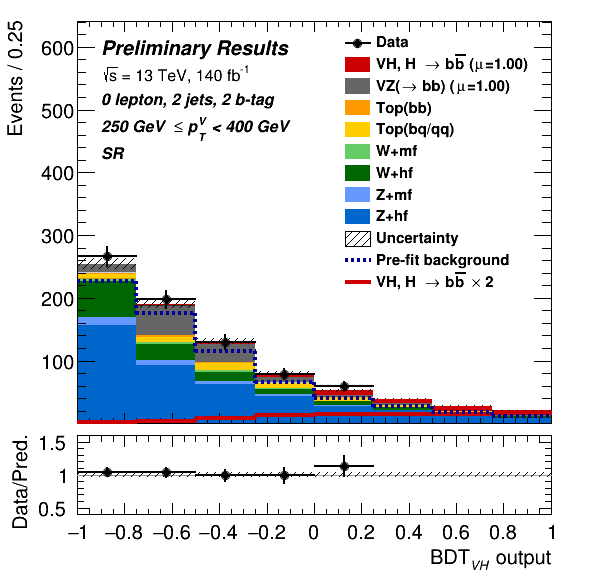
\includegraphics[width=0.32\textwidth]{Images/VH/postfit_VHbb/ZeroLep/Region_distmva_BMax400_BMin250_DSR_J2_TTypebb_T2_L0_Y6051_GlobalFit_conditionnal_mu1.pdf}
    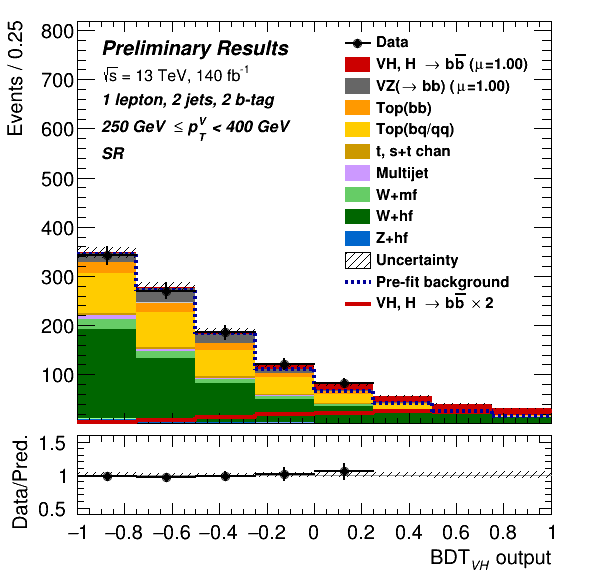
\includegraphics[width=0.32\textwidth]{ Images/VH/postfit_VHbb/OneLep/Region_distmva_BMax400_BMin250_DSR_J2_TTypebb_T2_L1_Y6051_GlobalFit_conditionnal_mu1.pdf}
    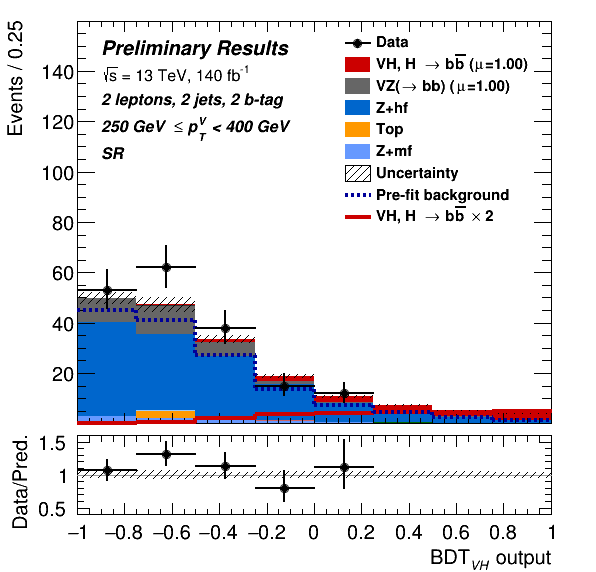
\includegraphics[width=0.32\textwidth]{ Images/VH/postfit_VHbb/TwoLep/Region_distmva_BMax400_BMin250_DSR_J2_TTypebb_T2_L2_Y6051_GlobalFit_conditionnal_mu1.pdf}
    \caption{The \vhb\ posfit conditional distribution in the 250 < \ptv\ < 400 GeV 2-jet signal region in the 0L (left), 1L (centre), and 2L (right).}
    \label{fig:plotsVHBSR_250pt_2J}
  \end{figure}
  
  \begin{figure}[h!]
    \centering
    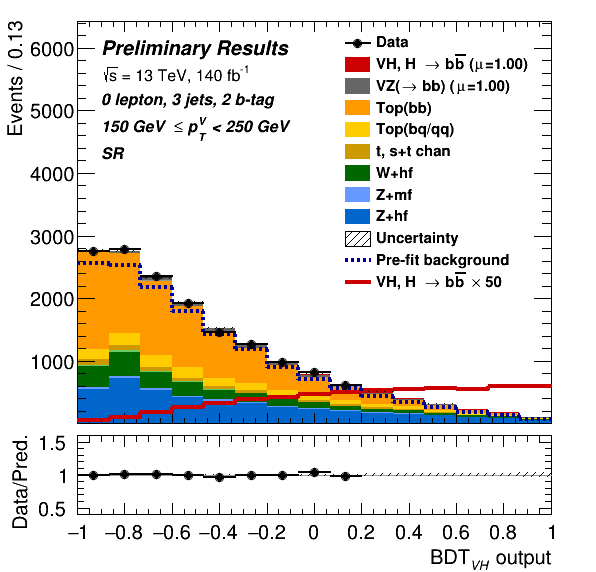
\includegraphics[width=0.32\textwidth]{Images/VH/postfit_VHbb/ZeroLep/Region_distmva_BMax250_BMin150_DSR_J3_TTypebb_T2_L0_Y6051_GlobalFit_conditionnal_mu1.pdf}
    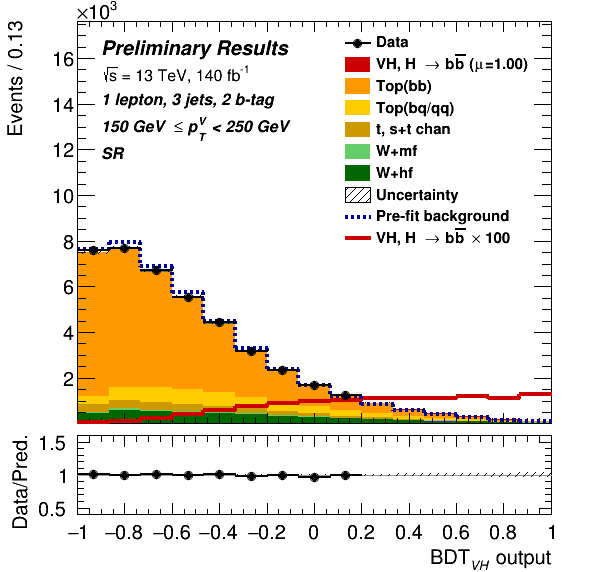
\includegraphics[width=0.32\textwidth]{Images/VH/postfit_VHbb/OneLep/Region_distmva_BMax250_BMin150_DSR_J3_TTypebb_T2_L1_Y6051_GlobalFit_conditionnal_mu1.pdf}
    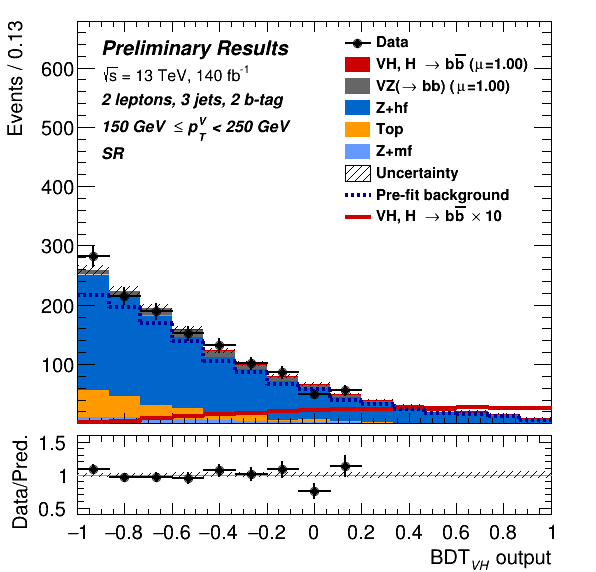
\includegraphics[width=0.32\textwidth]{Images/VH/postfit_VHbb/TwoLep/Region_distmva_BMax250_BMin150_DSR_J3_TTypebb_T2_L2_Y6051_GlobalFit_conditionnal_mu1.pdf}
    \caption{The \vhb\ posfit conditional distribution in the 150 < \ptv\ < 250 GeV 3-jet signal region in the 0L (left), 1L (centre), and 2L (right).}
    \label{fig:plotsVHBSR_150pt_3J}
  \end{figure} 
  
  \begin{figure}[h!]
    \centering
    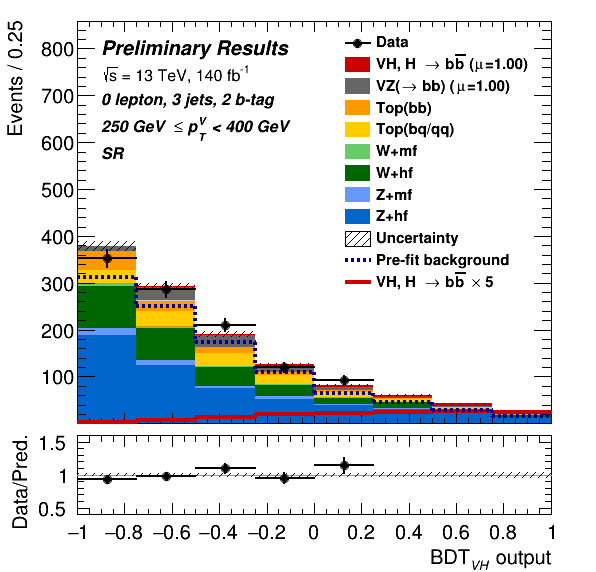
\includegraphics[width=0.32\textwidth]{Images/VH/postfit_VHbb/ZeroLep/Region_distmva_BMax400_BMin250_DSR_J3_TTypebb_T2_L0_Y6051_GlobalFit_conditionnal_mu1.pdf}
    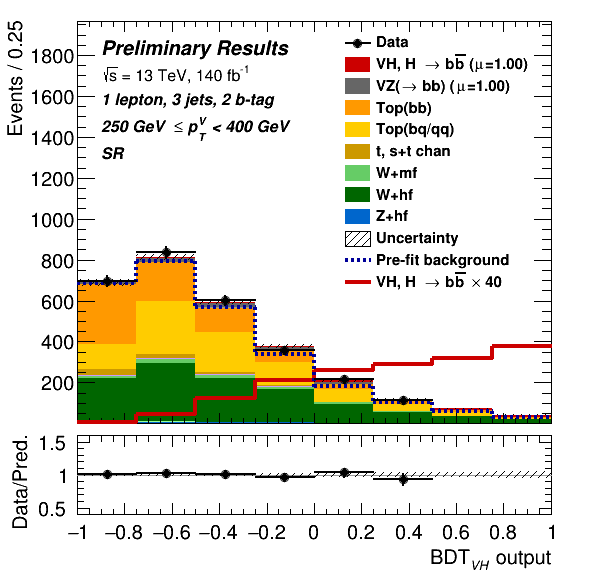
\includegraphics[width=0.32\textwidth]{ Images/VH/postfit_VHbb/OneLep/Region_distmva_BMax400_BMin250_DSR_J3_TTypebb_T2_L1_Y6051_GlobalFit_conditionnal_mu1.pdf}
    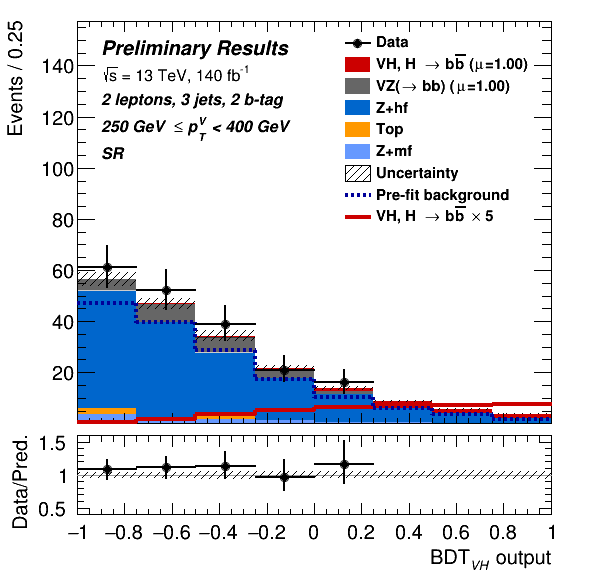
\includegraphics[width=0.32\textwidth]{ Images/VH/postfit_VHbb/TwoLep/Region_distmva_BMax400_BMin250_DSR_J3_TTypebb_T2_L2_Y6051_GlobalFit_conditionnal_mu1.pdf}
    \caption{The \vhb\ posfit conditional distribution in the 250 < \ptv\ < 400 GeV 3-jet signal region in the 0L (left), 1L (centre), and 2L (right).}
    \label{fig:plotsVHBSR_250pt_3J}
  \end{figure} 
  
  % 4J mid pTV
  \begin{figure}[h!]
    \centering
    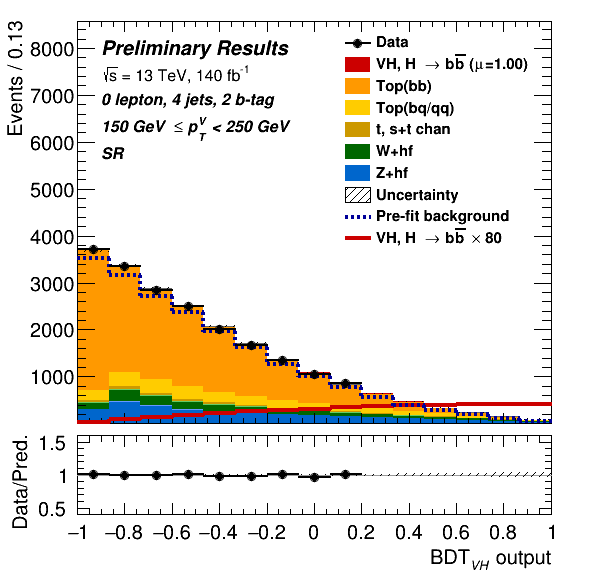
\includegraphics[width=0.24\textwidth]{Images/VH/postfit_VHbb/ZeroLep/Region_distmva_BMax250_BMin150_DSR_J4_TTypebb_T2_L0_Y6051_GlobalFit_conditionnal_mu1.pdf}
    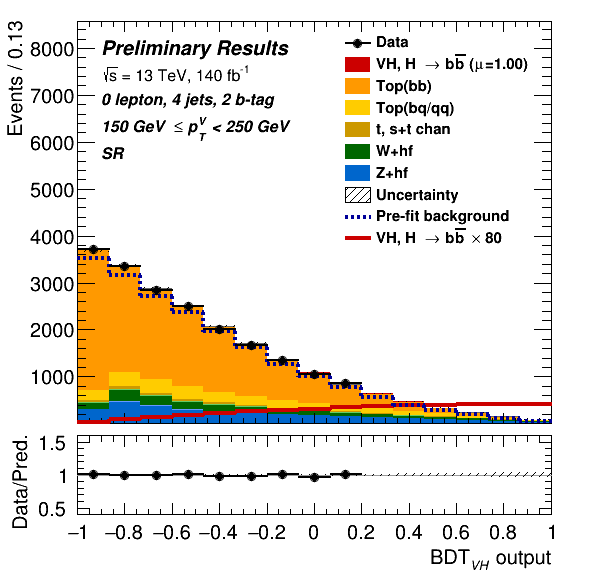
\includegraphics[width=0.24\textwidth]{Images/VH/postfit_VHbb/ZeroLep/Region_distmva_BMax250_BMin150_DSR_J4_TTypebb_T2_L0_Y6051_GlobalFit_conditionnal_mu1.pdf}
    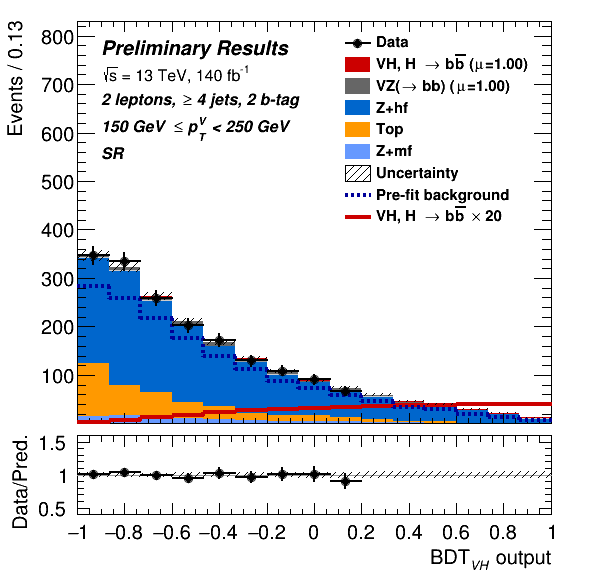
\includegraphics[width=0.24\textwidth]{ Images/VH/postfit_VHbb/TwoLep/Region_distmva_BMax250_BMin150_DSR_J4_TTypebb_incJet1_T2_L2_Y6051_GlobalFit_conditionnal_mu1.pdf}
    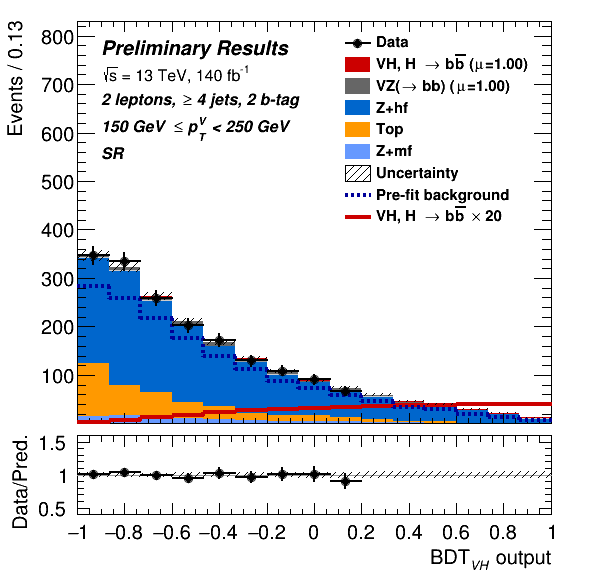
\includegraphics[width=0.24\textwidth]{ Images/VH/postfit_VHbb/TwoLep/Region_distmva_BMax250_BMin150_DSR_J4_TTypebb_incJet1_T2_L2_Y6051_GlobalFit_conditionnal_mu1.pdf}
    \caption{The \vhb\ posfit conditional distribution in the 150 < \ptv\ < 250 GeV 4-jet (4p-jet) signal region in the 0L (2 left) and 2L (2 right).}
    \label{fig:plotsVHBSR_150pt_4J}
  \end{figure} 
  
  \begin{figure}[h!]
    \centering
    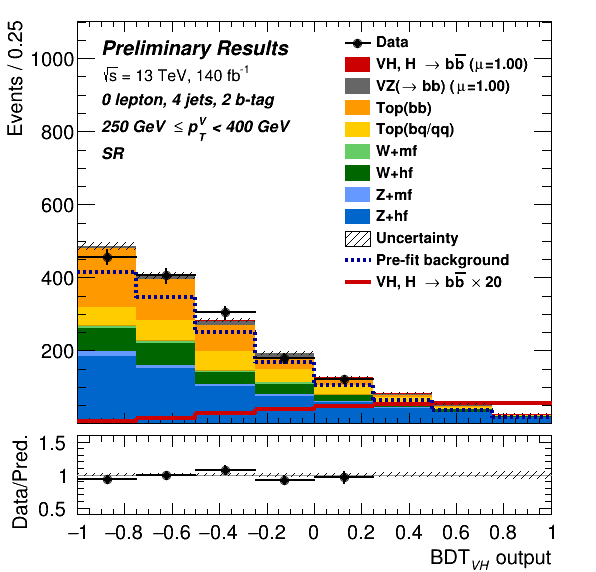
\includegraphics[width=0.24\textwidth]{Images/VH/postfit_VHbb/ZeroLep/Region_distmva_BMax400_BMin250_DSR_J4_TTypebb_T2_L0_Y6051_GlobalFit_conditionnal_mu1.pdf}
    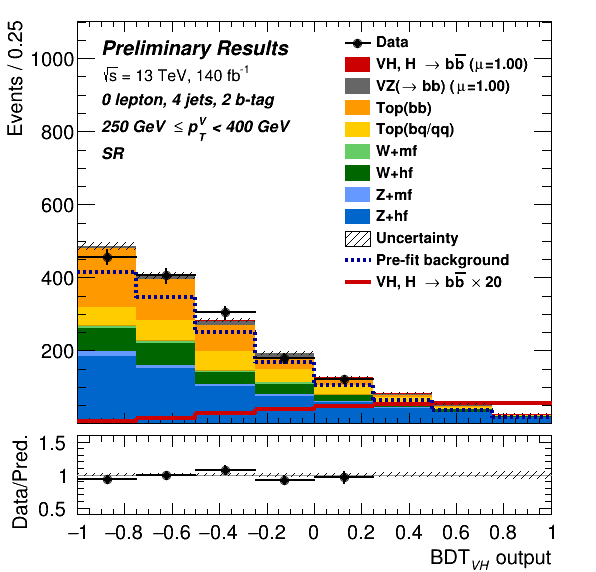
\includegraphics[width=0.24\textwidth]{Images/VH/postfit_VHbb/ZeroLep/Region_distmva_BMax400_BMin250_DSR_J4_TTypebb_T2_L0_Y6051_GlobalFit_conditionnal_mu1.pdf}
    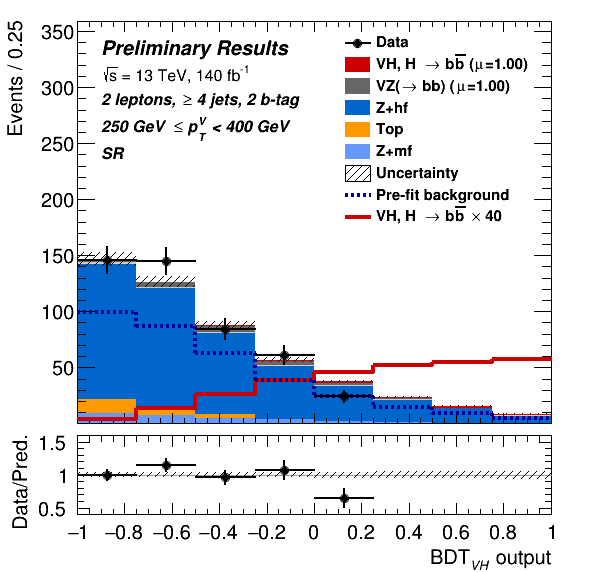
\includegraphics[width=0.24\textwidth]{ Images/VH/postfit_VHbb/TwoLep/Region_distmva_BMax400_BMin250_DSR_J4_TTypebb_incJet1_T2_L2_Y6051_GlobalFit_conditionnal_mu1.pdf}
    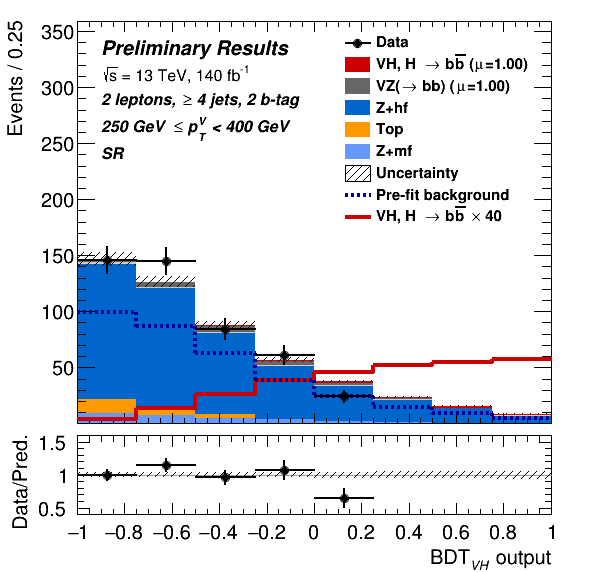
\includegraphics[width=0.24\textwidth]{ Images/VH/postfit_VHbb/TwoLep/Region_distmva_BMax400_BMin250_DSR_J4_TTypebb_incJet1_T2_L2_Y6051_GlobalFit_conditionnal_mu1.pdf}
    \caption{The \vhb\ posfit conditional distribution in the 150 < \ptv\ < 250 GeV 4-jet (4p-jet) signal region in the 0L (2 left) and 2L (2 right).}
    \label{fig:plotsVHBSR_250pt_4J}
  \end{figure} 
  
  % low pTV VHbb
  \begin{figure}[h!]
    \centering
    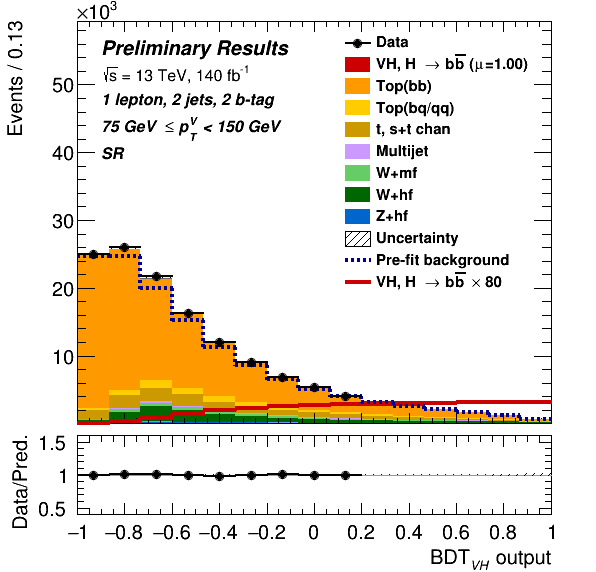
\includegraphics[width=0.32\textwidth]{Images/VH/postfit_VHbb/OneLep/Region_distmva_BMax150_BMin75_DSR_J2_TTypebb_T2_L1_Y6051_GlobalFit_conditionnal_mu1.pdf}
    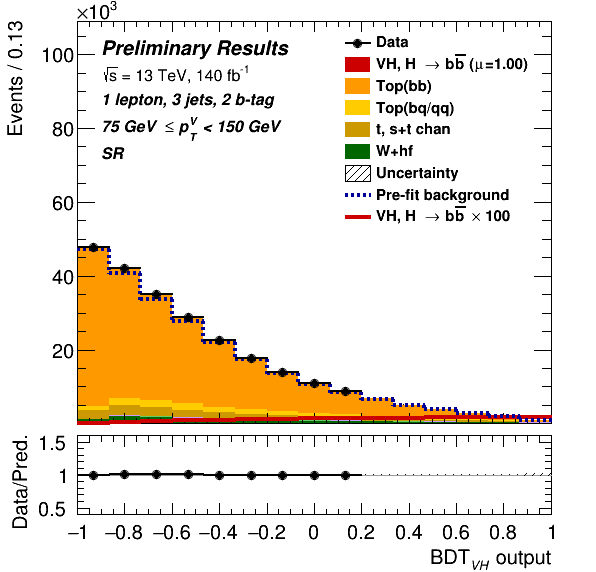
\includegraphics[width=0.32\textwidth]{Images/VH/postfit_VHbb/OneLep/Region_distmva_BMax150_BMin75_DSR_J3_TTypebb_T2_L1_Y6051_GlobalFit_conditionnal_mu1.pdf}
    \caption{The 1L \vhb\ posfit conditional distribution in the 75 < \ptv\ < 150 GeV 2-jet (left) and 3-jet (right) signal regions.}
    \label{fig:plotsVHBSR_75pt_1L}
  \end{figure} 
  
  \begin{figure}[h!]
    \centering
    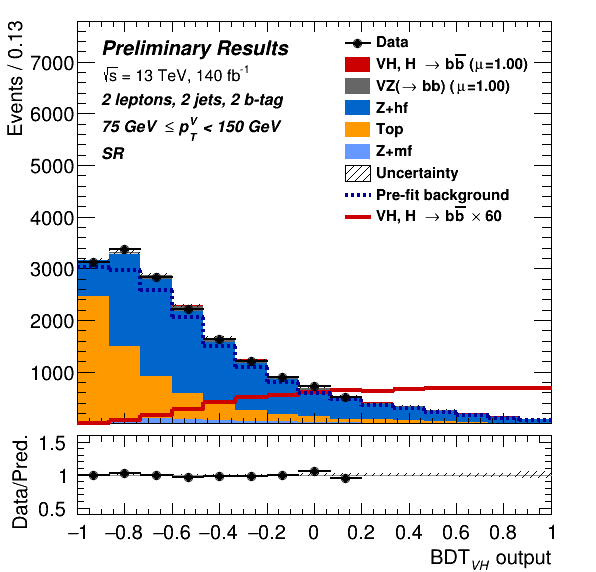
\includegraphics[width=0.32\textwidth]{Images/VH/postfit_VHbb/TwoLep/Region_distmva_BMax150_BMin75_DSR_J2_TTypebb_T2_L2_Y6051_GlobalFit_conditionnal_mu1.pdf}
    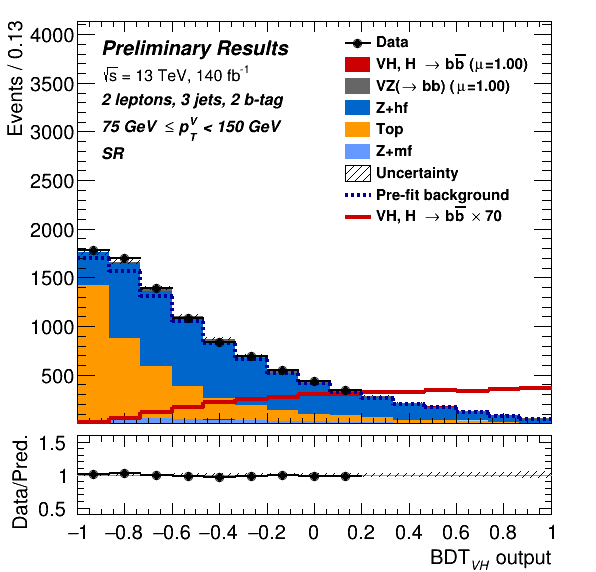
\includegraphics[width=0.32\textwidth]{Images/VH/postfit_VHbb/TwoLep/Region_distmva_BMax150_BMin75_DSR_J3_TTypebb_T2_L2_Y6051_GlobalFit_conditionnal_mu1.pdf}
    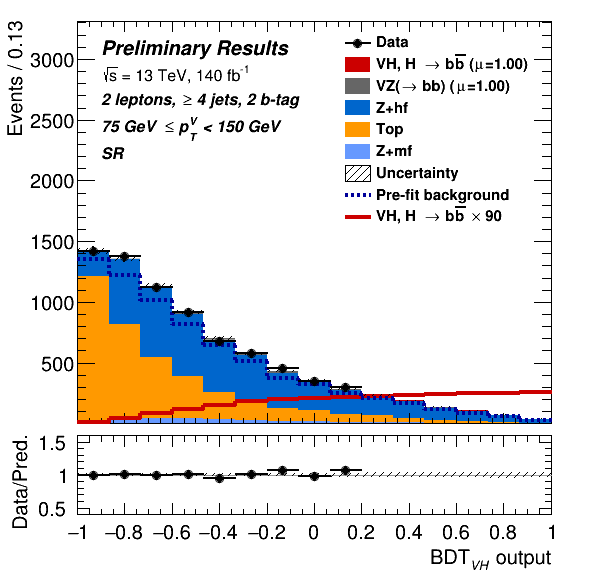
\includegraphics[width=0.32\textwidth]{Images/VH/postfit_VHbb/TwoLep/Region_distmva_BMax150_BMin75_DSR_J4_TTypebb_incJet1_T2_L2_Y6051_GlobalFit_conditionnal_mu1.pdf}
    \caption{The 2L \vhb\ posfit conditional distribution in the 75 < \ptv\ < 150 GeV 2-jet (left), 3-jet (centre) and 4p-jet (right) signal regions.}
    \label{fig:plotsVHBSR_75pt_2L}
  \end{figure} 
  
  %\begin{figure}[h!]
  %  \includegraphics[width=0.32\textwidth]{Images/VH/postfit_VHbb/ZeroLep/}
  %  \includegraphics[width=0.32\textwidth]{Images/VH/postfit_VHbb/OneLep/}
  %  \includegraphics[width=0.32\textwidth]{Images/VH/postfit_VHbb/TwoLep/}
  %  \caption{}
  %  \label{fig:plots}
  %\end{figure} 


 % ---


\begin{figure}[h!]
    \centering
    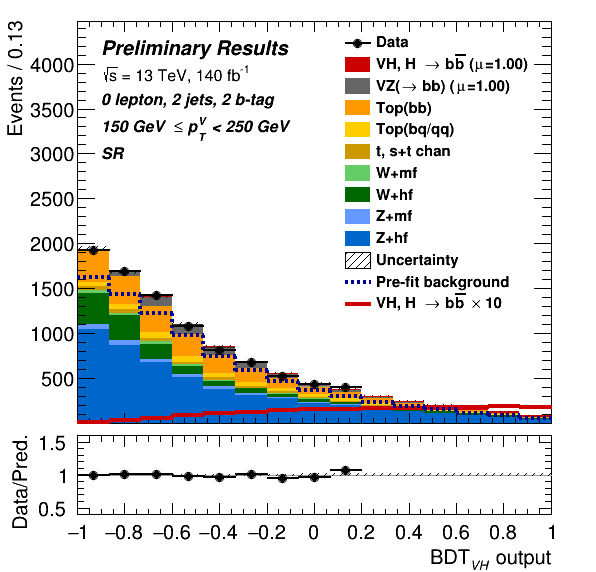
\includegraphics[width=0.32\textwidth]{Images/VH/postfit_VHbb/ZeroLep/Region_distmva_BMax250_BMin150_DSR_J2_TTypebb_T2_L0_Y6051_GlobalFit_conditionnal_mu1.pdf}
    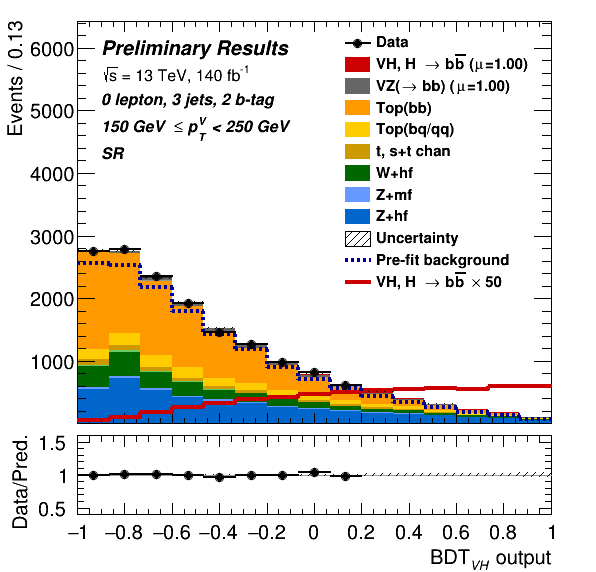
\includegraphics[width=0.32\textwidth]{Images/VH/postfit_VHbb/ZeroLep/Region_distmva_BMax250_BMin150_DSR_J3_TTypebb_T2_L0_Y6051_GlobalFit_conditionnal_mu1.pdf}
    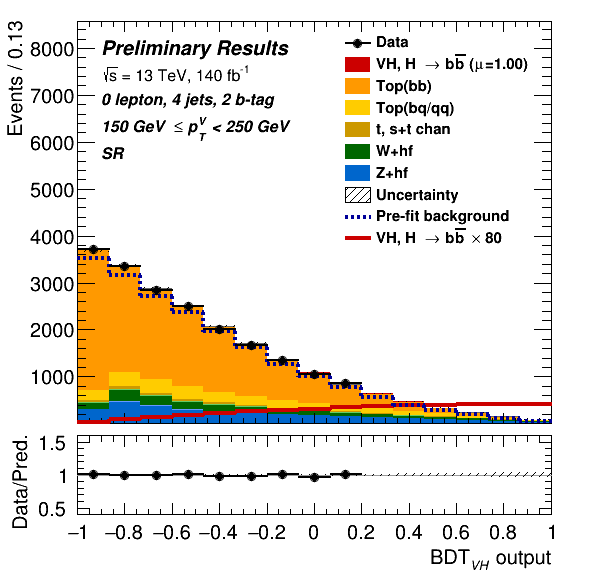
\includegraphics[width=0.32\textwidth]{Images/VH/postfit_VHbb/ZeroLep/Region_distmva_BMax250_BMin150_DSR_J4_TTypebb_T2_L0_Y6051_GlobalFit_conditionnal_mu1.pdf}
    \caption{The 0L posfit conditional distribution in the $BB$-tag, 150 < \ptv\ < 250 GeV, 2-jet(left), 3-jet (centre), and 4-jet (right) signal regions.}
    \label{fig:plotsVHBSR_150pt_0L}
\end{figure} 

\begin{figure}[h!]
    \centering
    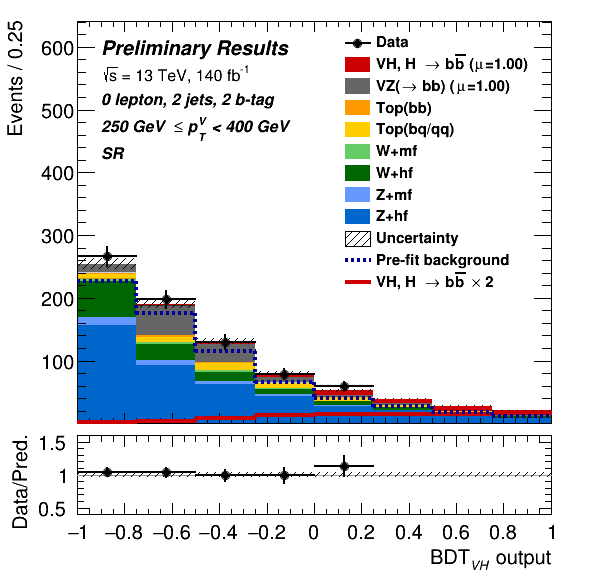
\includegraphics[width=0.32\textwidth]{Images/VH/postfit_VHbb/ZeroLep/Region_distmva_BMax400_BMin250_DSR_J2_TTypebb_T2_L0_Y6051_GlobalFit_conditionnal_mu1.pdf}
    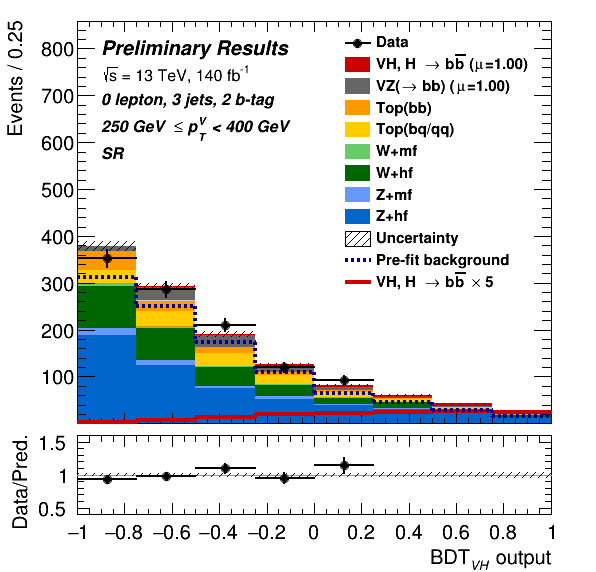
\includegraphics[width=0.32\textwidth]{Images/VH/postfit_VHbb/ZeroLep/Region_distmva_BMax400_BMin250_DSR_J3_TTypebb_T2_L0_Y6051_GlobalFit_conditionnal_mu1.pdf}
    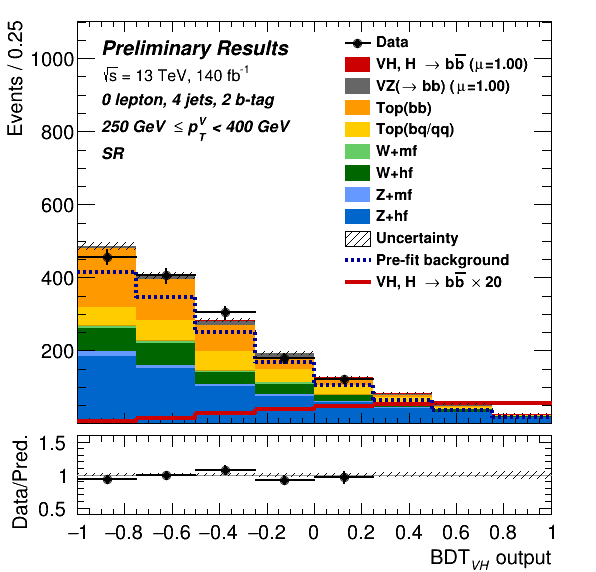
\includegraphics[width=0.32\textwidth]{Images/VH/postfit_VHbb/ZeroLep/Region_distmva_BMax400_BMin250_DSR_J4_TTypebb_T2_L0_Y6051_GlobalFit_conditionnal_mu1.pdf}
    \caption{The 0L posfit conditional distribution in the $BB$-tag, 250 < \ptv\ < 400 GeV, 2-jet(left), 3-jet (centre), and 4-jet (right) signal regions.}
    \label{fig:plotsVHBSR_250pt_0L}
\end{figure} 

\begin{figure}[h!]
    \centering
    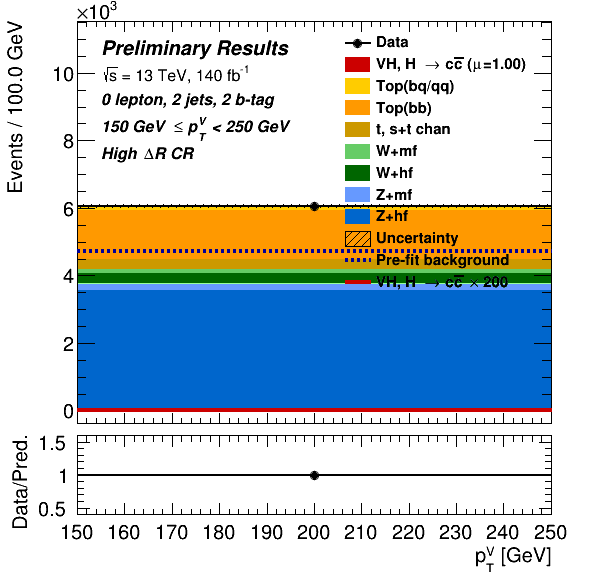
\includegraphics[width=0.32\textwidth]{Images/VH/postfit_VHbb/ZeroLep/Region_distpTV_BMax250_BMin150_DCRHigh_J2_TTypebb_T2_L0_Y6051_GlobalFit_conditionnal_mu1.pdf}
    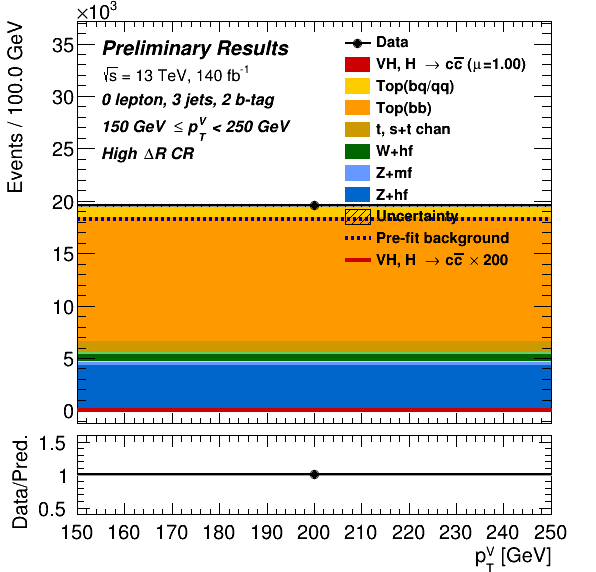
\includegraphics[width=0.32\textwidth]{Images/VH/postfit_VHbb/ZeroLep/Region_distpTV_BMax250_BMin150_DCRHigh_J3_TTypebb_T2_L0_Y6051_GlobalFit_conditionnal_mu1.pdf}
    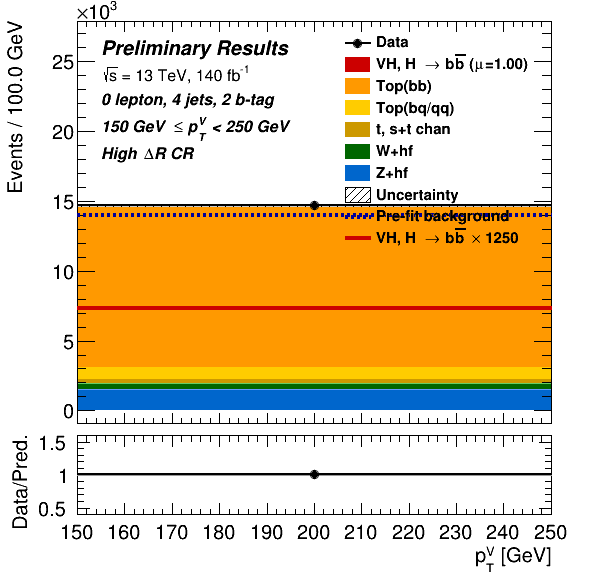
\includegraphics[width=0.32\textwidth]{Images/VH/postfit_VHbb/ZeroLep/Region_distpTV_BMax250_BMin150_DCRHigh_J4_TTypebb_T2_L0_Y6051_GlobalFit_conditionnal_mu1.pdf}
    \caption{The 0L posfit conditional distribution in the $BB$-tag, 150 < \ptv\ < 250 GeV 2-jet(left), 3-jet (centre), and 4-jet (right) signal regions.}
    \label{fig:plotsVHBSR_150pt_0L}
\end{figure} 


Region_distpTV_BMax250_BMin150_DCRHigh_J2_TTypebb_T2_L0_Y6051_GlobalFit_conditionnal_mu1.pdf
Region_distpTV_BMax250_BMin150_DCRHigh_J3_TTypebb_T2_L0_Y6051_GlobalFit_conditionnal_mu1.pdf
Region_distpTV_BMax250_BMin150_DCRHigh_J4_TTypebb_T2_L0_Y6051_GlobalFit_conditionnal_mu1.pdf

Region_distpTV_BMax400_BMin250_DCRHigh_J2_TTypebb_T2_L0_Y6051_GlobalFit_conditionnal_mu1.pdf
Region_distpTV_BMax400_BMin250_DCRHigh_J3_TTypebb_T2_L0_Y6051_GlobalFit_conditionnal_mu1.pdf
Region_distpTV_BMax400_BMin250_DCRHigh_J4_TTypebb_T2_L0_Y6051_GlobalFit_conditionnal_mu1.pdf
\clearpage 
% 0L  
\vspace*{\fill}

\begin{figure}[h!]
    \centering
    \begin{subfigure}[b]{\textwidth}
        \centering
        \includegraphics[width=0.32\textwidth]{Images/VH/Own_fit/postfit_VHcc/Region_distmva_BMax250_BMin150_DSR_J2_TTypext_T2_L0_Y6051_GlobalFit_conditionnal_mu1.png}
        \includegraphics[width=0.32\textwidth]{Images/VH/Own_fit/postfit_VHcc/Region_distmva_BMax250_BMin150_DSR_J3_TTypext_T2_L0_Y6051_GlobalFit_conditionnal_mu1.png}
        \caption{150 < \ptv\ < 250 GeV.}
        \label{fig:plots_VHcc_OL_150_SR_2c}
    \end{subfigure}
    \begin{subfigure}[b]{\textwidth}
        \centering
        \includegraphics[width=0.32\textwidth]{Images/VH/Own_fit/postfit_VHcc/Region_distmva_BMin250_DSR_J2_TTypext_T2_L0_Y6051_GlobalFit_conditionnal_mu1.png}
        \includegraphics[width=0.32\textwidth]{Images/VH/Own_fit/postfit_VHcc/Region_distmva_BMin250_DSR_J3_TTypext_T2_L0_Y6051_GlobalFit_conditionnal_mu1.png}
        \caption{250 GeV < \ptv.}
        \label{fig:plots_VHcc_OL_250_SR_2c}
    \end{subfigure}
    \caption{\gls{bdt} distributions in the 0L 2 $c$-tagged signal regions, 2-jet (left) and 3-jet (right).}
    \label{fig:plots_VHcc_OL_SR_2c}
\end{figure} 
\begin{figure}[h!]
    \centering
    \begin{subfigure}[b]{\textwidth}
        \centering
        \includegraphics[width=0.32\textwidth]{Images/VH/Own_fit/postfit_VHcc/Region_distmva_BMax250_BMin150_DSR_J2_TTypent_T1_L0_Y6051_GlobalFit_conditionnal_mu1.png}
        \includegraphics[width=0.32\textwidth]{Images/VH/Own_fit/postfit_VHcc/Region_distmva_BMax250_BMin150_DSR_J3_TTypent_T1_L0_Y6051_GlobalFit_conditionnal_mu1.png}
        \caption{150 < \ptv\ < 250 GeV.}
        \label{fig:plots_VHcc_OL_150_SR_1c}
    \end{subfigure}
    \begin{subfigure}[b]{\textwidth}
        \centering
        \includegraphics[width=0.32\textwidth]{Images/VH/Own_fit/postfit_VHcc/Region_distmva_BMin250_DSR_J2_TTypent_T1_L0_Y6051_GlobalFit_conditionnal_mu1.png}
        \includegraphics[width=0.32\textwidth]{Images/VH/Own_fit/postfit_VHcc/Region_distmva_BMin250_DSR_J3_TTypent_T1_L0_Y6051_GlobalFit_conditionnal_mu1.png}
        \caption{250 GeV < \ptv.}
        \label{fig:plots_VHcc_OL_250_SR_1c}
    \end{subfigure}
    \caption{\gls{bdt} distributions in the 0L 1 $c$-tagged signal regions, 2-jet (left) and 3-jet (right).}
    \label{fig:plots_VHcc_OL_SR_1c}
\end{figure} 

\vspace*{\fill} 

\begin{figure}[h!]
    \centering
    \begin{subfigure}[b]{\textwidth}
        \centering
        \includegraphics[width=0.32\textwidth]{Images/VH/Own_fit/postfit_VHcc/Region_distmBB_BMax250_BMin150_DCRHigh_J2_TTypent_T1_L0_Y6051_GlobalFit_conditionnal_mu1.png}
        \includegraphics[width=0.32\textwidth]{Images/VH/Own_fit/postfit_VHcc/Region_distmBB_BMax250_BMin150_DCRHigh_J2_TTypelt_T2_L0_Y6051_GlobalFit_conditionnal_mu1.png}
        \includegraphics[width=0.32\textwidth]{Images/VH/Own_fit/postfit_VHcc/Region_distmBB_BMax250_BMin150_DCRHigh_J2_TTypett_T2_L0_Y6051_GlobalFit_conditionnal_mu1.png}
        \caption{150 < \ptv\ < 250 GeV, $TN$- (left), $LT$- (centre), and $TT$-tag (right).}
        \label{fig:plots_VHcc_OL_150_CRH_2c_2J}
    \end{subfigure}
    \begin{subfigure}[b]{\textwidth}
        \centering
        \includegraphics[width=0.32\textwidth]{Images/VH/Own_fit/postfit_VHcc/Region_distmBB_BMin250_DCRHigh_J2_TTypent_T1_L0_Y6051_GlobalFit_conditionnal_mu1.png}
        \includegraphics[width=0.32\textwidth]{Images/VH/Own_fit/postfit_VHcc/Region_distmBB_BMin250_DCRHigh_J2_TTypelt_T2_L0_Y6051_GlobalFit_conditionnal_mu1.png}
        \includegraphics[width=0.32\textwidth]{Images/VH/Own_fit/postfit_VHcc/Region_distmBB_BMin250_DCRHigh_J2_TTypett_T2_L0_Y6051_GlobalFit_conditionnal_mu1.png}
        \caption{250 GeV < \ptv, $TN$- (left), $LT$- (centre), and $TT$-tag (right).}
        \label{fig:plots_VHcc_OL_250_CRH_2c_2J}
    \end{subfigure}
    \caption{$H$-candidate mass distributions in the 0L 2-jet \highdr\ CRs.}
    \label{fig:plots_VHcc_OL_CRH_2c_2J}
\end{figure} 
\begin{figure}[h!]
    \centering
    \begin{subfigure}[b]{\textwidth}
        \centering
        \includegraphics[width=0.32\textwidth]{Images/VH/Own_fit/postfit_VHcc/Region_distmBB_BMax250_BMin150_DCRHigh_J3_TTypent_T1_L0_Y6051_GlobalFit_conditionnal_mu1.png}
        \includegraphics[width=0.32\textwidth]{Images/VH/Own_fit/postfit_VHcc/Region_distmBB_BMax250_BMin150_DCRHigh_J3_TTypelt_T2_L0_Y6051_GlobalFit_conditionnal_mu1.png}
        \includegraphics[width=0.32\textwidth]{Images/VH/Own_fit/postfit_VHcc/Region_distmBB_BMax250_BMin150_DCRHigh_J3_TTypett_T2_L0_Y6051_GlobalFit_conditionnal_mu1.png}
        \caption{150 GeV < \ptv\ < 250 GeV, $TN$- (left), $LT$- (centre), and $TT$-tag (right).}
        \label{fig:plots_VHcc_OL_150_CRH_2c_3J}
    \end{subfigure}
    \begin{subfigure}[b]{\textwidth}
        \centering

        \includegraphics[width=0.32\textwidth]{Images/VH/Own_fit/postfit_VHcc/Region_distmBB_BMin250_DCRHigh_J3_TTypent_T1_L0_Y6051_GlobalFit_conditionnal_mu1.png}
        \includegraphics[width=0.32\textwidth]{Images/VH/Own_fit/postfit_VHcc/Region_distmBB_BMin250_DCRHigh_J3_TTypelt_T2_L0_Y6051_GlobalFit_conditionnal_mu1.png}
        \includegraphics[width=0.32\textwidth]{Images/VH/Own_fit/postfit_VHcc/Region_distmBB_BMin250_DCRHigh_J3_TTypett_T2_L0_Y6051_GlobalFit_conditionnal_mu1.png}
        \caption{250 GeV < \ptv, $TN$- (left), $LT$- (centre), and $TT$-tag (right).}
        \label{fig:plots_VHcc_OL_250_CRH_2c_3J}
    \end{subfigure}
    \caption{$H$-candidate mass distributions in the 0L 3-jet \highdr\ CRs.}
    \label{fig:plots_VHcc_OL_CRH_2c_3J}
\end{figure} 

\vspace*{\fill} 

% TopCR 0L
\begin{figure}[h!]
    \centering
    \begin{subfigure}[b]{\textwidth}
        \centering
        \includegraphics[width=0.32\textwidth]{Images/VH/Own_fit/postfit_VHcc/Region_distmBB_BMax250_BMin150_DtopCRBC_J2_TTypebt_T1_L0_Y6051_GlobalFit_conditionnal_mu1.png}
        \includegraphics[width=0.32\textwidth]{Images/VH/Own_fit/postfit_VHcc/Region_distmBB_BMax250_BMin150_DtopCRBC_J3_TTypebt_T1_L0_Y6051_GlobalFit_conditionnal_mu1.png}
        \includegraphics[width=0.32\textwidth]{Images/VH/Own_fit/postfit_VHbb/Region_distmBB_BMax250_BMin150_DtopCRBC_J4_TTypebt_T1_L0_Y6051_GlobalFit_conditionnal_mu1.png} % Must be VHbb due to 4j
        \caption{150 < \ptv\ < 250 GeV.}
        \label{fig:plots_VHcc_OL_150_TopCR_2c}
    \end{subfigure}
    \begin{subfigure}[b]{\textwidth}
        \centering
        \includegraphics[width=0.32\textwidth]{Images/VH/Own_fit/postfit_VHcc/Region_distmBB_BMax400_BMin250_DtopCRBC_J2_TTypebt_T1_L0_Y6051_GlobalFit_conditionnal_mu1.png}
        \includegraphics[width=0.32\textwidth]{Images/VH/Own_fit/postfit_VHcc/Region_distmBB_BMax400_BMin250_DtopCRBC_J3_TTypebt_T1_L0_Y6051_GlobalFit_conditionnal_mu1.png}
        \includegraphics[width=0.32\textwidth]{Images/VH/Own_fit/postfit_VHbb/Region_distmBB_BMax400_BMin250_DtopCRBC_J4_TTypebt_T1_L0_Y6051_GlobalFit_conditionnal_mu1.png} % Must be VHbb due to 4j
        \caption{250 GeV < \ptv\ < 400 GeV.}
        \label{fig:plots_VHcc_OL_250_TopCR_2c}
    \end{subfigure}
    \caption{$H$-candidate mass distributions in the 0L $BT$-tagged Top CRs, 2-jet (left), 3-jet (centre), and 4-jet (right).}
    \label{fig:plots_VHcc_OL_TopCR_2c}
\end{figure} 

\vspace*{\fill} \newpage
\vspace*{\fill} 

% 1L
\begin{figure}[h!]
    \centering
    \begin{subfigure}[b]{\textwidth}
        \centering
        \includegraphics[width=0.32\textwidth]{Images/VH/Own_fit/postfit_VHcc/Region_distmva_BMax150_BMin75_DSR_J2_TTypext_T2_L1_Y6051_GlobalFit_conditionnal_mu1.png}
        \includegraphics[width=0.32\textwidth]{Images/VH/Own_fit/postfit_VHcc/Region_distmva_BMax250_BMin150_DSR_J2_TTypext_T2_L1_Y6051_GlobalFit_conditionnal_mu1.png}
        \includegraphics[width=0.32\textwidth]{Images/VH/Own_fit/postfit_VHcc/Region_distmva_BMin250_DSR_J2_TTypext_T2_L1_Y6051_GlobalFit_conditionnal_mu1.png}
        \caption{2-jet, [75, 150] GeV (left), [150, 250] GeV (centre), and 250  GeV $\leq$ (right) \ptv\ regions.}
        \label{fig:plots_VHcc_1L_SR_2J_2c}
    \end{subfigure}
    \begin{subfigure}[b]{\textwidth}
        \centering
        \includegraphics[width=0.32\textwidth]{Images/VH/Own_fit/postfit_VHcc/Region_distmva_BMax150_BMin75_DSR_J3_TTypext_T2_L1_Y6051_GlobalFit_conditionnal_mu1.png}
        \includegraphics[width=0.32\textwidth]{Images/VH/Own_fit/postfit_VHcc/Region_distmva_BMax250_BMin150_DSR_J3_TTypext_T2_L1_Y6051_GlobalFit_conditionnal_mu1.png}
        \includegraphics[width=0.32\textwidth]{Images/VH/Own_fit/postfit_VHcc/Region_distmva_BMin250_DSR_J3_TTypext_T2_L1_Y6051_GlobalFit_conditionnal_mu1.png}
        \caption{3-jet, [75, 150] GeV (left), [150, 250] GeV (centre), and 250  GeV $\leq$ (right) \ptv\ regions.}
        \label{fig:plots_VHcc_1L_SR_3J_2c}
    \end{subfigure}
    \caption{\gls{bdt} distributions in the 1L 2 $c$-tagged signal regions.}
    \label{fig:plots_VHcc_1L_SR_2c}
\end{figure}
\begin{figure}[h!]
    \centering
    \begin{subfigure}[b]{\textwidth}
        \centering
        \includegraphics[width=0.32\textwidth]{Images/VH/Own_fit/postfit_VHcc/Region_distmva_BMax250_BMin150_DSR_J2_TTypent_T1_L1_Y6051_GlobalFit_conditionnal_mu1.png}
        \includegraphics[width=0.32\textwidth]{Images/VH/Own_fit/postfit_VHcc/Region_distmva_BMin250_DSR_J2_TTypent_T1_L1_Y6051_GlobalFit_conditionnal_mu1.png}
        \caption{2-jet, [75, 150] GeV (left), [150, 250] GeV (centre), and 250  GeV $\leq$ (right) \ptv\ regions.}
        \label{fig:plots_VHcc_1L_SR_2J_1c}
    \end{subfigure}
    \begin{subfigure}[b]{\textwidth}
        \centering
        \includegraphics[width=0.32\textwidth]{Images/VH/Own_fit/postfit_VHcc/Region_distmva_BMax250_BMin150_DSR_J3_TTypent_T1_L1_Y6051_GlobalFit_conditionnal_mu1.png}
        \includegraphics[width=0.32\textwidth]{Images/VH/Own_fit/postfit_VHcc/Region_distmva_BMin250_DSR_J3_TTypent_T1_L1_Y6051_GlobalFit_conditionnal_mu1.png}
        \caption{3-jet, [75, 150] GeV (left), [150, 250] GeV (centre), and 250  GeV $\leq$ (right) \ptv\ regions.}
        \label{fig:plots_VHcc_1L_SR_3J_1c}
    \end{subfigure}
    \caption{\gls{bdt} distributions in the 1L 1 $c$-tagged signal regions.}
    \label{fig:plots_VHcc_1L_SR_1c}
\end{figure}

\newpage
\vspace*{\fill} 


\begin{figure}[h!]
    \centering
    \begin{subfigure}[b]{\textwidth}
        \centering
        \includegraphics[width=0.32\textwidth]{Images/VH/Own_fit/blank.png}
        \includegraphics[width=0.32\textwidth]{Images/VH/Own_fit/postfit_VHcc/Region_distmBB_BMax150_BMin75_DCRHigh_J2_TTypelt_T2_L1_Y6051_GlobalFit_conditionnal_mu1.png}
        \includegraphics[width=0.32\textwidth]{Images/VH/Own_fit/postfit_VHcc/Region_distmBB_BMax150_BMin75_DCRHigh_J2_TTypett_T2_L1_Y6051_GlobalFit_conditionnal_mu1.png}
        \caption{75 < \ptv\ < 150 GeV ($TN$ not included).}
        \label{fig:plots_VHcc_1L_75_CRH_2J}
    \end{subfigure}
    \begin{subfigure}[b]{\textwidth}
        \centering
        \includegraphics[width=0.32\textwidth]{Images/VH/Own_fit/postfit_VHcc/Region_distpTV_BMax250_BMin150_DCRHigh_J2_TTypent_T1_L1_Y6051_GlobalFit_conditionnal_mu1.png}
        \includegraphics[width=0.32\textwidth]{Images/VH/Own_fit/postfit_VHcc/Region_distmBB_BMax250_BMin150_DCRHigh_J2_TTypelt_T2_L1_Y6051_GlobalFit_conditionnal_mu1.png}
        \includegraphics[width=0.32\textwidth]{Images/VH/Own_fit/postfit_VHcc/Region_distmBB_BMax250_BMin150_DCRHigh_J2_TTypett_T2_L1_Y6051_GlobalFit_conditionnal_mu1.png}
        \caption{150 < \ptv\ < 250 GeV.}
        \label{fig:plots_VHcc_1L_150_CRH_2J}
    \end{subfigure}
    \begin{subfigure}[b]{\textwidth}
        \centering
        \includegraphics[width=0.32\textwidth]{Images/VH/Own_fit/postfit_VHcc/Region_distpTV_BMin250_DCRHigh_J2_TTypent_T1_L1_Y6051_GlobalFit_conditionnal_mu1.png}
        \includegraphics[width=0.32\textwidth]{Images/VH/Own_fit/postfit_VHcc/Region_distmBB_BMin250_DCRHigh_J2_TTypelt_T2_L1_Y6051_GlobalFit_conditionnal_mu1.png}
        \includegraphics[width=0.32\textwidth]{Images/VH/Own_fit/postfit_VHcc/Region_distmBB_BMin250_DCRHigh_J2_TTypett_T2_L1_Y6051_GlobalFit_conditionnal_mu1.png}
        \caption{250 GeV < \ptv.}
        \label{fig:plots_VHcc_1L_250_CRH_2J}
    \end{subfigure}
    \caption{$TN$-tagged \ptv\ distributions (left) and $LT$- (centre) and $TT$-tagged (right) $H$-candidate mass distributions in the 1L \highdr\ CR 2-jet regions.}
    \label{fig:plots_VHcc_1L_CRH_2J}
\end{figure}

\vspace*{\fill} \newpage
\vspace*{\fill} 

\begin{figure}[h!]
    \centering
    \begin{subfigure}[b]{\textwidth}
        \centering
        \includegraphics[width=0.32\textwidth]{Images/VH/Own_fit/blank.png}
        \includegraphics[width=0.32\textwidth]{Images/VH/Own_fit/postfit_VHcc/Region_distmBB_BMax150_BMin75_DCRHigh_J3_TTypelt_T2_L1_Y6051_GlobalFit_conditionnal_mu1.png}
        \includegraphics[width=0.32\textwidth]{Images/VH/Own_fit/postfit_VHcc/Region_distmBB_BMax150_BMin75_DCRHigh_J3_TTypett_T2_L1_Y6051_GlobalFit_conditionnal_mu1.png}
        \caption{75 < \ptv\ < 150 GeV ($TN$ not included).}
        \label{fig:plots_VHcc_1L_75_CRH_3J}
    \end{subfigure}
    \begin{subfigure}[b]{\textwidth}
        \centering
        \includegraphics[width=0.32\textwidth]{Images/VH/Own_fit/postfit_VHcc/Region_distpTV_BMax250_BMin150_DCRHigh_J3_TTypent_T1_L1_Y6051_GlobalFit_conditionnal_mu1.png}
        \includegraphics[width=0.32\textwidth]{Images/VH/Own_fit/postfit_VHcc/Region_distmBB_BMax250_BMin150_DCRHigh_J3_TTypelt_T2_L1_Y6051_GlobalFit_conditionnal_mu1.png}
        \includegraphics[width=0.32\textwidth]{Images/VH/Own_fit/postfit_VHcc/Region_distmBB_BMax250_BMin150_DCRHigh_J3_TTypett_T2_L1_Y6051_GlobalFit_conditionnal_mu1.png}
        \caption{150 < \ptv\ < 250 GeV.}
        \label{fig:plots_VHcc_1L_150_CRH_3J}
    \end{subfigure}
    \begin{subfigure}[b]{\textwidth}
        \centering
        \includegraphics[width=0.32\textwidth]{Images/VH/Own_fit/postfit_VHcc/Region_distpTV_BMin250_DCRHigh_J3_TTypent_T1_L1_Y6051_GlobalFit_conditionnal_mu1.png}
        \includegraphics[width=0.32\textwidth]{Images/VH/Own_fit/postfit_VHcc/Region_distmBB_BMin250_DCRHigh_J3_TTypelt_T2_L1_Y6051_GlobalFit_conditionnal_mu1.png}
        \includegraphics[width=0.32\textwidth]{Images/VH/Own_fit/postfit_VHcc/Region_distmBB_BMin250_DCRHigh_J3_TTypett_T2_L1_Y6051_GlobalFit_conditionnal_mu1.png}
        \caption{250 GeV < \ptv.}
        \label{fig:plots_VHcc_1L_250_CRH_3J}
    \end{subfigure}
    \caption{$TN$-tagged \ptv\ distributions (left) and $LT$- (centre) and $TT$-tagged (right) $H$-candidate mass distributions in the 1L \highdr\ CR 3-jet regions.}
    \label{fig:plots_VHcc_1L_CRH_3J}
\end{figure}

\vspace*{\fill} \newpage

\begin{figure}[h!]
    \centering
    \begin{subfigure}[b]{\textwidth}
        \centering
        \includegraphics[width=0.32\textwidth]{Images/VH/Own_fit/postfit_VHcc/Region_distmBB_BMax150_BMin75_DtopCRBC_J2_TTypebt_T1_L1_Y6051_GlobalFit_conditionnal_mu1.png}
        \includegraphics[width=0.32\textwidth]{Images/VH/Own_fit/postfit_VHcc/Region_distmBB_BMax250_BMin150_DtopCRBC_J2_TTypebt_T1_L1_Y6051_GlobalFit_conditionnal_mu1.png}
        \includegraphics[width=0.32\textwidth]{Images/VH/Own_fit/postfit_VHcc/Region_distmBB_BMax400_BMin250_DtopCRBC_J2_TTypebt_T1_L1_Y6051_GlobalFit_conditionnal_mu1.png}
        \caption{2-jet, [75, 150] GeV (left), [150, 250] GeV (centre), and 250 GeV $\leq$ (right) \ptv\ regions.}
        \label{fig:plots_VHcc_1L_TopCR_2J}
    \end{subfigure}
    \begin{subfigure}[b]{\textwidth}
        \centering
        \includegraphics[width=0.32\textwidth]{Images/VH/Own_fit/postfit_VHcc/Region_distmBB_BMax150_BMin75_DtopCRBC_J3_TTypebt_T1_L1_Y6051_GlobalFit_conditionnal_mu1.png}
        \includegraphics[width=0.32\textwidth]{Images/VH/Own_fit/postfit_VHcc/Region_distmBB_BMax250_BMin150_DtopCRBC_J3_TTypebt_T1_L1_Y6051_GlobalFit_conditionnal_mu1.png}
        \includegraphics[width=0.32\textwidth]{Images/VH/Own_fit/postfit_VHcc/Region_distmBB_BMax400_BMin250_DtopCRBC_J3_TTypebt_T1_L1_Y6051_GlobalFit_conditionnal_mu1.png}
        \caption{3-jet, [75, 150] GeV (left), [150, 250] GeV (centre), and 250 GeV $\leq$ (right) \ptv\ regions.}
        \label{fig:plots_VHcc_1L_TopCR_3J}
    \end{subfigure}
    \caption{$H$-candidate mass distribution in the 1L $BT$-tagged Top CRs.}
    \label{fig:plots_VHcc_1L_TopCR}
\end{figure}
\begin{figure}[h!]
    \centering
    \begin{subfigure}[b]{\textwidth}
        \centering
        \includegraphics[width=0.32\textwidth]{Images/VH/Own_fit/postfit_VHcc/Region_distpTV_BMax250_BMin150_DSR_J2_TTypeln_T1_L1_Y6051_GlobalFit_conditionnal_mu1.png}
        \includegraphics[width=0.32\textwidth]{Images/VH/Own_fit/postfit_VHcc/Region_distpTV_BMin250_DSR_J2_TTypeln_T1_L1_Y6051_GlobalFit_conditionnal_mu1.png}
        \caption{2-jet.}
        \label{fig:plots_VHcc_1L_LN_2J}
    \end{subfigure}
    \begin{subfigure}[b]{\textwidth}
        \centering
        \includegraphics[width=0.32\textwidth]{Images/VH/Own_fit/postfit_VHcc/Region_distpTV_BMax250_BMin150_DSR_J3_TTypeln_T1_L1_Y6051_GlobalFit_conditionnal_mu1.png}
        \includegraphics[width=0.32\textwidth]{Images/VH/Own_fit/postfit_VHcc/Region_distpTV_BMin250_DSR_J3_TTypeln_T1_L1_Y6051_GlobalFit_conditionnal_mu1.png}
        \caption{3-jet.}
        \label{fig:plots_VHcc_1L_SR_3J}
    \end{subfigure}
    \caption{\ptv\ distributions in the 1L $LN$-tagged $V+l$ CR [150, 250] GeV (left) and 250 GeV $\leq$ (right) \ptv\ regions.}
    \label{fig:plots_VHcc_1L_LN}
\end{figure}

\newpage

% 2L
\vspace*{\fill} 

\begin{figure}[h!]
    \centering
    \begin{subfigure}[b]{\textwidth}
        \centering
        \includegraphics[width=0.32\textwidth]{Images/VH/Own_fit/postfit_VHcc/Region_distmva_BMax150_BMin75_DSR_J2_TTypext_T2_L2_Y6051_GlobalFit_conditionnal_mu1.png}
        \includegraphics[width=0.32\textwidth]{Images/VH/Own_fit/postfit_VHcc/Region_distmva_BMax250_BMin150_DSR_J2_TTypext_T2_L2_Y6051_GlobalFit_conditionnal_mu1.png}
        \includegraphics[width=0.32\textwidth]{Images/VH/Own_fit/postfit_VHcc/Region_distmva_BMin250_DSR_J2_TTypext_T2_L2_Y6051_GlobalFit_conditionnal_mu1.png}
        \caption{2-jet, [75, 150] GeV (left), [150, 250] GeV (centre), and 250  GeV $\leq$ (right) \ptv\ regions.}
        \label{fig:plots_VHcc_2L_SR_2c_2J}
    \end{subfigure}
    \begin{subfigure}[b]{\textwidth}
        \centering
        \includegraphics[width=0.32\textwidth]{Images/VH/Own_fit/postfit_VHcc/Region_distmva_BMax150_BMin75_DSR_J3_TTypext_incJet1_T2_L2_Y6051_GlobalFit_conditionnal_mu1.png}
        \includegraphics[width=0.32\textwidth]{Images/VH/Own_fit/postfit_VHcc/Region_distmva_BMax250_BMin150_DSR_J3_TTypext_incJet1_T2_L2_Y6051_GlobalFit_conditionnal_mu1.png}
        \includegraphics[width=0.32\textwidth]{Images/VH/Own_fit/postfit_VHcc/Region_distmva_BMin250_DSR_J3_TTypext_incJet1_T2_L2_Y6051_GlobalFit_conditionnal_mu1.png}
        \caption{$\geq$3-jet, [75, 150] GeV (left), [150, 250] GeV (centre), and 250  GeV $\leq$ (right) \ptv\ regions.}
        \label{fig:plots_VHcc_2L_SR_2c_3J}
    \end{subfigure}
    \caption{\gls{bdt} distributions in the 2L 2 $c$-tagged signal regions.}
    \label{fig:plots_VHcc_2L_SR_2c}
\end{figure}
\begin{figure}[h!]
    \centering
    \begin{subfigure}[b]{\textwidth}
        \centering
        \includegraphics[width=0.32\textwidth]{Images/VH/Own_fit/postfit_VHcc/Region_distmva_BMax150_BMin75_DSR_J2_TTypent_T1_L2_Y6051_GlobalFit_conditionnal_mu1.png}
        \includegraphics[width=0.32\textwidth]{Images/VH/Own_fit/postfit_VHcc/Region_distmva_BMax250_BMin150_DSR_J2_TTypent_T1_L2_Y6051_GlobalFit_conditionnal_mu1.png}
        \includegraphics[width=0.32\textwidth]{Images/VH/Own_fit/postfit_VHcc/Region_distmva_BMin250_DSR_J2_TTypent_T1_L2_Y6051_GlobalFit_conditionnal_mu1.png}
        \caption{2-jet, [75, 150] GeV (left), [150, 250] GeV (centre), and 250  GeV $\leq$ (right) \ptv\ regions.}
        \label{fig:plots_VHcc_2L_SR_1c_2J}
    \end{subfigure}
    \begin{subfigure}[b]{\textwidth}
        \centering
        \includegraphics[width=0.32\textwidth]{Images/VH/Own_fit/postfit_VHcc/Region_distmva_BMax150_BMin75_DSR_J3_TTypent_incJet1_T1_L2_Y6051_GlobalFit_conditionnal_mu1.png}
        \includegraphics[width=0.32\textwidth]{Images/VH/Own_fit/postfit_VHcc/Region_distmva_BMax250_BMin150_DSR_J3_TTypent_incJet1_T1_L2_Y6051_GlobalFit_conditionnal_mu1.png}
        \includegraphics[width=0.32\textwidth]{Images/VH/Own_fit/postfit_VHcc/Region_distmva_BMin250_DSR_J3_TTypent_incJet1_T1_L2_Y6051_GlobalFit_conditionnal_mu1.png}
        \caption{$\geq$3-jet, [75, 150] GeV (left), [150, 250] GeV (centre), and 250  GeV $\leq$ (right) \ptv\ regions.}
        \label{fig:plots_VHcc_2L_SR_1c_3J}
    \end{subfigure}
    \caption{\gls{bdt} distributions in the 2L 1 $c$-tagged signal regions.}
    \label{fig:plots_VHcc_2L_SR_1c}
\end{figure}

\newpage
\vspace*{\fill} 


\begin{figure}[h!]
    \centering
    \begin{subfigure}[b]{\textwidth}
        \centering
        \includegraphics[width=0.32\textwidth]{Images/VH/Own_fit/postfit_VHcc/Region_distpTV_BMax150_BMin75_DCRHigh_J2_TTypent_T1_L2_Y6051_GlobalFit_conditionnal_mu1.png}
        \includegraphics[width=0.32\textwidth]{Images/VH/Own_fit/postfit_VHcc/Region_distmBB_BMax150_BMin75_DCRHigh_J2_TTypelt_T2_L2_Y6051_GlobalFit_conditionnal_mu1.png}
        \includegraphics[width=0.32\textwidth]{Images/VH/Own_fit/postfit_VHcc/Region_distmBB_BMax150_BMin75_DCRHigh_J2_TTypett_T2_L2_Y6051_GlobalFit_conditionnal_mu1.png}
        \caption{75 < \ptv\ < 150 GeV.}
        \label{fig:plots_VHcc_2L_75_CRH_2J}
    \end{subfigure}
    \begin{subfigure}[b]{\textwidth}
        \centering
        \includegraphics[width=0.32\textwidth]{Images/VH/Own_fit/postfit_VHcc/Region_distpTV_BMax250_BMin150_DCRHigh_J2_TTypent_T1_L2_Y6051_GlobalFit_conditionnal_mu1.png}
        \includegraphics[width=0.32\textwidth]{Images/VH/Own_fit/postfit_VHcc/Region_distmBB_BMax250_BMin150_DCRHigh_J2_TTypelt_T2_L2_Y6051_GlobalFit_conditionnal_mu1.png}
        \includegraphics[width=0.32\textwidth]{Images/VH/Own_fit/postfit_VHcc/Region_distmBB_BMax250_BMin150_DCRHigh_J2_TTypett_T2_L2_Y6051_GlobalFit_conditionnal_mu1.png}
        \caption{150 < \ptv\ < 250 GeV.}
        \label{fig:plots_VHcc_2L_150_CRH_2J}
    \end{subfigure}
    \begin{subfigure}[b]{\textwidth}
        \centering
        \includegraphics[width=0.32\textwidth]{Images/VH/Own_fit/postfit_VHcc/Region_distpTV_BMin250_DCRHigh_J2_TTypent_T1_L2_Y6051_GlobalFit_conditionnal_mu1.png}
        \includegraphics[width=0.32\textwidth]{Images/VH/Own_fit/postfit_VHcc/Region_distmBB_BMin250_DCRHigh_J2_TTypelt_T2_L2_Y6051_GlobalFit_conditionnal_mu1.png}
        \includegraphics[width=0.32\textwidth]{Images/VH/Own_fit/postfit_VHcc/Region_distmBB_BMin250_DCRHigh_J2_TTypett_T2_L2_Y6051_GlobalFit_conditionnal_mu1.png}
        \caption{250 GeV < \ptv.}
        \label{fig:plots_VHcc_2L_250_CRH_2J}
    \end{subfigure}
    \caption{$TN$-tagged \ptv\ distributions (left) and the $LT$- (centre) and $TT$-tagged (right) $H$-candidate mass distributions in the 2L \highdr\ CR 2-jet regions.}
    \label{fig:plots_VHcc_2L_CRH_3J}
\end{figure}

\vspace*{\fill} \newpage
\vspace*{\fill} 

\begin{figure}[h!]
    \centering
    \begin{subfigure}[b]{\textwidth}
        \centering
        \includegraphics[width=0.32\textwidth]{Images/VH/Own_fit/postfit_VHcc/Region_distpTV_BMax150_BMin75_DCRHigh_J3_TTypent_incJet1_T1_L2_Y6051_GlobalFit_conditionnal_mu1.png}
        \includegraphics[width=0.32\textwidth]{Images/VH/Own_fit/postfit_VHcc/Region_distmBB_BMax150_BMin75_DCRHigh_J3_TTypelt_incJet1_T2_L2_Y6051_GlobalFit_conditionnal_mu1.png}
        \includegraphics[width=0.32\textwidth]{Images/VH/Own_fit/postfit_VHcc/Region_distmBB_BMax150_BMin75_DCRHigh_J3_TTypett_incJet1_T2_L2_Y6051_GlobalFit_conditionnal_mu1.png}
        \caption{75 < \ptv\ < 150 GeV.}
        \label{fig:plots_VHcc_2L_75_CRH_3J}
    \end{subfigure}
    \begin{subfigure}[b]{\textwidth}
        \centering
        \includegraphics[width=0.32\textwidth]{Images/VH/Own_fit/postfit_VHcc/Region_distpTV_BMax250_BMin150_DCRHigh_J3_TTypent_incJet1_T1_L2_Y6051_GlobalFit_conditionnal_mu1.png}
        \includegraphics[width=0.32\textwidth]{Images/VH/Own_fit/postfit_VHcc/Region_distmBB_BMax250_BMin150_DCRHigh_J3_TTypelt_incJet1_T2_L2_Y6051_GlobalFit_conditionnal_mu1.png}
        \includegraphics[width=0.32\textwidth]{Images/VH/Own_fit/postfit_VHcc/Region_distmBB_BMax250_BMin150_DCRHigh_J3_TTypett_incJet1_T2_L2_Y6051_GlobalFit_conditionnal_mu1.png}
        \caption{150 < \ptv\ < 250 GeV.}
        \label{fig:plots_VHcc_2L_150_CRH_3J}
    \end{subfigure}
    \begin{subfigure}[b]{\textwidth}
        \centering
        \includegraphics[width=0.32\textwidth]{Images/VH/Own_fit/postfit_VHcc/Region_distpTV_BMin250_DCRHigh_J3_TTypent_incJet1_T1_L2_Y6051_GlobalFit_conditionnal_mu1.png}
        \includegraphics[width=0.32\textwidth]{Images/VH/Own_fit/postfit_VHcc/Region_distmBB_BMin250_DCRHigh_J3_TTypelt_incJet1_T2_L2_Y6051_GlobalFit_conditionnal_mu1.png}
        \includegraphics[width=0.32\textwidth]{Images/VH/Own_fit/postfit_VHcc/Region_distmBB_BMin250_DCRHigh_J3_TTypett_incJet1_T2_L2_Y6051_GlobalFit_conditionnal_mu1.png}
        \caption{250 GeV < \ptv.}
        \label{fig:plots_VHcc_2L_250_CRH_3J}
    \end{subfigure}
    \caption{$TN$-tagged \ptv\ distributions (left) and the $LT$- (centre) and $TT$-tagged (right) $H$-candidate mass distributions in the 2L \highdr\ CR 3-jet regions.}
    \label{fig:plots_VHcc_2L_CRH_3J}
\end{figure}

\vspace*{\fill} \newpage
\vspace*{\fill} 

\begin{figure}[h!]
    \centering
    \begin{subfigure}[b]{\textwidth}
        \centering
        \includegraphics[width=0.32\textwidth]{Images/VH/Own_fit/postfit_VHcc/Region_distpTV_BMax150_BMin75_DSR_J2_TTypeln_T1_L2_Y6051_GlobalFit_conditionnal_mu1.png}
        \includegraphics[width=0.32\textwidth]{Images/VH/Own_fit/postfit_VHcc/Region_distpTV_BMax250_BMin150_DSR_J2_TTypeln_T1_L2_Y6051_GlobalFit_conditionnal_mu1.png}
        \includegraphics[width=0.32\textwidth]{Images/VH/Own_fit/postfit_VHcc/Region_distpTV_BMin250_DSR_J2_TTypeln_T1_L2_Y6051_GlobalFit_conditionnal_mu1.png}
        \caption{2-jet, [75, 150] GeV (left), [150, 250] GeV (centre), and 250  GeV $\leq$ (right) \ptv\ regions.}
        \label{fig:plots_VHcc_2L_LN_2J}
    \end{subfigure}
    \begin{subfigure}[b]{\textwidth}
        \centering
        \includegraphics[width=0.32\textwidth]{Images/VH/Own_fit/postfit_VHcc/Region_distpTV_BMax150_BMin75_DSR_J3_TTypeln_incJet1_T1_L2_Y6051_GlobalFit_conditionnal_mu1.png}
        \includegraphics[width=0.32\textwidth]{Images/VH/Own_fit/postfit_VHcc/Region_distpTV_BMax250_BMin150_DSR_J3_TTypeln_incJet1_T1_L2_Y6051_GlobalFit_conditionnal_mu1.png}
        \includegraphics[width=0.32\textwidth]{Images/VH/Own_fit/postfit_VHcc/Region_distpTV_BMin250_DSR_J3_TTypeln_incJet1_T1_L2_Y6051_GlobalFit_conditionnal_mu1.png}
        \caption{$\geq$3-jet, [75, 150] GeV (left), [150, 250] GeV (centre), and 250  GeV $\leq$ (right) \ptv\ regions.}
        \label{fig:plots_VHcc_2L_LN_3J}
    \end{subfigure}
    \caption{\ptv\ distributions in the 2L $LN$-tagged $V+l$ CRs.}
    \label{fig:plots_VHcc_2L_LN}
\end{figure}

\begin{figure}[h!]
    \centering
    \begin{subfigure}[b]{\textwidth}
        \centering
        \includegraphics[width=0.32\textwidth]{Images/VH/Own_fit/postfit_VHcc/Region_distpTV_BMax150_BMin75_Dtopemucr_J2_TTypeta_T2_L2_Y6051_GlobalFit_conditionnal_mu1.png}
        \includegraphics[width=0.32\textwidth]{Images/VH/Own_fit/postfit_VHcc/Region_distpTV_BMax250_BMin150_Dtopemucr_J2_TTypeta_T2_L2_Y6051_GlobalFit_conditionnal_mu1.png}
        \includegraphics[width=0.32\textwidth]{Images/VH/Own_fit/postfit_VHcc/Region_distpTV_BMax400_BMin250_Dtopemucr_J2_TTypeta_T2_L2_Y6051_GlobalFit_conditionnal_mu1.png}
        \caption{2-jet, [75, 150] GeV (left), [150, 250] GeV (centre), and 250  GeV $\leq$ (right) \ptv\ regions.}
        \label{fig:plots_VHcc_2L_topCRemu_2J}
    \end{subfigure}
    \begin{subfigure}[b]{\textwidth}
        \centering
        \includegraphics[width=0.32\textwidth]{Images/VH/Own_fit/postfit_VHcc/Region_distpTV_BMax150_BMin75_Dtopemucr_J3_TTypeta_T2_L2_Y6051_GlobalFit_conditionnal_mu1.png}
        \includegraphics[width=0.32\textwidth]{Images/VH/Own_fit/postfit_VHcc/Region_distpTV_BMax250_BMin150_Dtopemucr_J3_TTypeta_T2_L2_Y6051_GlobalFit_conditionnal_mu1.png}
        \includegraphics[width=0.32\textwidth]{Images/VH/Own_fit/postfit_VHcc/Region_distpTV_BMax400_BMin250_Dtopemucr_J3_TTypeta_T2_L2_Y6051_GlobalFit_conditionnal_mu1.png}
        \caption{$\geq$3-jet, [75, 150] GeV (left), [150, 250] GeV (centre), and 250  GeV $\leq$ (right) \ptv\ regions.}
        \label{fig:plots_VHcc_2L_topCRemu_3J}
    \end{subfigure}
    \caption{\ptv\ distributions in the 2L Top $e\mu$ CR with $\geq$1 $T$-tagged regions.}
    \label{fig:plots_VHcc_2L_topCRemu}
\end{figure}

\clearpage
% 0L
\begin{figure}[h!]
    \centering
    \begin{subfigure}[b]{\textwidth}
        \centering
        \includegraphics[width=0.32\textwidth]{Images/VH/Own_fit/postfit_VHbb/Region_distmva_BMax600_BMin400_incFat1_Fat1_DSRnoaddbjetsr_J0_TTypebb_T2_L0_Y6051_GlobalFit_conditionnal_mu1.png
                                                                              Region_distmva_BMax600_BMin400_incFat1_Fat1_DSRnoaddbjetsr_J0_TTypebb_incJet1_T2_L0_Y6051_GlobalFit_conditionnal_mu1.png
        \includegraphics[width=0.32\textwidth]{Images/VH/Own_fit/postfit_VHbb/Region_distmva_BMax600_BMin400_incFat1_Fat1_DSRnoaddbjetsr_J1_TTypebb_incJet1_T2_L0_Y6051_GlobalFit_conditionnal_mu1.png}
        \includegraphics[width=0.32\textwidth]{Images/VH/Own_fit/postfit_VHbb/Region_distmva_BMin600_incFat1_Fat1_DSRnoaddbjetsr_J0_TTypebb_incJet1_T2_L0_Y6051_GlobalFit_conditionnal_mu1.png}
        \caption{The \ptv\ $\in$ [400, 600] GeV high- and low-purity (left and centre) and the \ptv\ $\geq$ 600 GeV (right) signal regions.}
        \label{fig:plots_VHbbBoost_OL_SR}
    \end{subfigure}
    \begin{subfigure}[b]{\textwidth}
        \centering
        \includegraphics[width=0.32\textwidth]{Images/VH/Own_fit/postfit_VHbb/Region_distmBB_BMax600_BMin400_incFat1_Fat1_DSRtopaddbjetcr_J0_TTypebb_incJet1_T2_L0_Y6051_GlobalFit_conditionnal_mu1.png}
        \includegraphics[width=0.32\textwidth]{Images/VH/Own_fit/postfit_VHbb/Region_distmBB_BMin600_incFat1_Fat1_DSRtopaddbjetcr_J0_TTypebb_incJet1_T2_L0_Y6051_GlobalFit_conditionnal_mu1.png}
        \caption{The \ptv\ $\in$ [400, 600] GeV (left) and \ptv\ $\geq$ 600 GeV (right) boosted Top CR.}
        \label{fig:plots_VHbbBoost_OL_topCR}
    \end{subfigure}
    \caption{The boosted $BB$-tagged 0L regions.}
    \label{fig:plots_VHbbBoost_OL}
\end{figure} 


% 1L

\begin{figure}[h!]
    \centering
    \begin{subfigure}[b]{\textwidth}
        \centering
        \includegraphics[width=0.32\textwidth]{Images/VH/Own_fit/postfit_VHbb/Region_distmva_BMax600_BMin400_incFat1_Fat1_DSRnoaddbjetsr_J0_TTypebb_T2_L1_Y6051_GlobalFit_conditionnal_mu1.png}
        \includegraphics[width=0.32\textwidth]{Images/VH/Own_fit/postfit_VHbb/Region_distmva_BMax600_BMin400_incFat1_Fat1_DSRnoaddbjetsr_J1_TTypebb_incJet1_T2_L1_Y6051_GlobalFit_conditionnal_mu1.png}
        \includegraphics[width=0.32\textwidth]{Images/VH/Own_fit/postfit_VHbb/Region_distmva_BMin600_incFat1_Fat1_DSRnoaddbjetsr_J0_TTypebb_incJet1_T2_L1_Y6051_GlobalFit_conditionnal_mu1.png}
        \caption{The \ptv\ $\in$ [400, 600] GeV high- and low-purity (left and centre) and the \ptv\ $\geq$ 600 GeV (right) signal regions.}
        \label{fig:plots_VHbbBoost_1L_SR}
    \end{subfigure}
    \begin{subfigure}[b]{\textwidth}
        \centering
        \includegraphics[width=0.32\textwidth]{Images/VH/Own_fit/postfit_VHbb/Region_distmBB_BMax600_BMin400_incFat1_Fat1_DSRtopaddbjetcr_J0_TTypebb_incJet1_T2_L1_Y6051_GlobalFit_conditionnal_mu1.png}
        \includegraphics[width=0.32\textwidth]{Images/VH/Own_fit/postfit_VHbb/Region_distmBB_BMin600_incFat1_Fat1_DSRtopaddbjetcr_J0_TTypebb_incJet1_T2_L1_Y6051_GlobalFit_conditionnal_mu1.png}
        \caption{The \ptv\ $\in$ [400, 600] GeV (left) and \ptv\ $\geq$ 600 GeV (right) boosted Top CR.}
        \label{fig:plots_VHbbBoost_1L_topCR}
    \end{subfigure}
    \caption{The boosted $BB$-tagged 0L regions.}
    \label{fig:plots_VHbbBoost_1L}
\end{figure} 

% 2L
\vspace*{\fill}

\begin{figure}[h!]
    \centering
    \includegraphics[width=0.32\textwidth]{Images/VH/Own_fit/postfit_VHbb/Region_distmva_BMax600_BMin400_incFat1_Fat1_DSR_J0_TTypebb_incJet1_T2_L2_Y6051_GlobalFit_conditionnal_mu1.png}
    \includegraphics[width=0.32\textwidth]{Images/VH/Own_fit/postfit_VHbb/Region_distmva_BMin600_incFat1_Fat1_DSR_J0_TTypebb_incJet1_T2_L2_Y6051_GlobalFit_conditionnal_mu1.png}
    \caption{The boosted $BB$-tagged 2L signal regions, \ptv\ $\in$ [400, 600] (left) and \ptv\ $\geq$ 600 GeV (right).}
    \label{fig:plots_VHbbBoost_2L_SR}
\end{figure} 

